%%%%%%%%%%%%%%%%%%%%%%%%%%%%%%%%%%%%%%%%%%%%%%%
%
% Template for Master degrees
% DISI - Dipartimento di Ingegneria e Scienza dell’Informazione
% DISI - Department of Information Engineering and Computer Science
%
% update 2020-08-30
%
% To generate pdf 
% pdflatex __filename__.tex
% bibtex __file_name__.aux
% pdflatex __file_name__.tex
% pdflatex __file_name__.tex
%
%%%%%%%%%%%%%%%%%%%%%%%%%%%%%%%%%%%%%%%%%%%%%%%

% 2 side format
\documentclass[epsfig,a4paper,11pt,titlepage,twoside,openany]{book}
\usepackage{epsfig}
\usepackage{plain}
\usepackage{setspace}
\usepackage[paperheight=29.7cm,paperwidth=21cm,outer=1.5cm,inner=2.5cm,top=2cm,bottom=2cm]{geometry} % layout setting
\usepackage{titlesec} % custom setup title of chanpter
% \usepackage{newtxtext,newtxmath} % times new roman

%%%%%%%%%%%%%%
% support for accented letters
%
%\usepackage[latin1]{inputenc} % Windows;
\usepackage[utf8x]{inputenc} % Linux (unicode package is required);
%\usepackage[applemac]{inputenc} % Mac.

\usepackage{cite}
\usepackage{graphicx}
\usepackage{algorithmic}
\usepackage{amsmath}
\usepackage{amsfonts} % for "\mathbb" macro
% \usepackage[caption=false,font=normalsize,labelfont=sf,textfont=sf]{subfig}
\usepackage{subcaption}
\usepackage{url}
\usepackage{hyperref}
\usepackage{float}
\usepackage{listings}
\usepackage{bm}
\usepackage{color}
\usepackage{cleveref}
\definecolor{codegreen}{rgb}{0,0.6,0}
\definecolor{codegray}{rgb}{0.5,0.5,0.5}
\definecolor{codeorange}{rgb}{1,0.49,0}
\definecolor{backcolour}{rgb}{0.95,0.95,0.96}

\lstset{
  backgroundcolor=\color{backcolour},   
  commentstyle=\color{codegray},
  keywordstyle=\color{codeorange},
  numberstyle=\tiny\color{codegray},
  stringstyle=\color{codegreen},
  basicstyle=\ttfamily\footnotesize,
  breakatwhitespace=false,         
  breaklines=true,                 
  captionpos=b,                    
  keepspaces=true,                 
  numbers=left,                    
  numbersep=5pt,                  
  showspaces=false,                
  showstringspaces=false,
  showtabs=false,                  
  tabsize=2,
  xleftmargin=10pt,
}
\renewcommand{\lstlistingname}{Code}

%to write code:
%\begin{lstlisting}[language=python, caption={my caption}]
%    
%\end{lstlisting}

\newcommand{\N}{\mathbb{N}}
\newcommand{\Z}{\mathbb{Z}}
\newcommand{\Q}{\mathbb{Q}}
\newcommand{\R}{\mathbb{R}}
\newcommand{\C}{\mathbb{C}}

\DeclareMathOperator*{\argmin}{arg\,min}
\DeclareMathOperator*{\argmax}{arg\,max}
\DeclareMathOperator{\nullop}{null}
\DeclareMathOperator{\rank}{rank}

\singlespacing

% italian language
%\usepackage[italian]{babel}


\let\subsubsection\subsection
\let\subsection\section
\let\section\chapter

\begin{document}

% no page number
\pagenumbering{gobble}
\pagestyle{plain}

\thispagestyle{empty}

\begin{center}
  \begin{figure}[h!]
    \centerline{
\psfig{file=marchio_unitrento_colore_it_202002.eps,width=0.6\textwidth}}
  \end{figure}

  \vspace{2 cm}

  \LARGE{Department of Information Engineering and Computer Science\\}

  \vspace{1 cm}
  \Large{Master's Degree in\\
    Computer Science
    % Computer, Communication and Electronic Engineering
    % Information and Communications Engineering
    % Information and Business Organization Engineering
    % Electornics and Telecommunications Engineerign
  }

  \vspace{2 cm}
  \Large\textsc{Final Dissertation\\}
  \vspace{1 cm}
  \Huge\textsc{MIMO physical layer security using multiple Reconfigurable Intelligence Surfaces\\}
  \vspace{1 cm}
  \Large{\it{A study in vehicular environments}}


  \vspace{2 cm}
  \begin{tabular*}{\textwidth}{ c @{\extracolsep{\fill}} c }
    \Large{Supervisor} & \Large{Student}\\
    \Large{Segata Michele} & \Large{Marrocco Simone}\\
    & \\
    \Large{Co-Supervisor} & \\
    \Large{Casari Paolo} & \\
  \end{tabular*}

  \vspace{2 cm}

  \Large{Academic year 2023/2024}

\end{center}



\clearpage

%%%%%%%%%%%%%%%%%%%%%%%%%%%%%%%%%%%%%%%%%%%%%%%%%%%%%%%%%%%%%%%%%%%%%%%%%%
%%%%%%%%%%%%%%%%%%%%%%%%%%%%%%%%%%%%%%%%%%%%%%%%%%%%%%%%%%%%%%%%%%%%%%%%%%
%% Note
%%%%%%%%%%%%%%%%%%%%%%%%%%%%%%%%%%%%%%%%%%%%%%%%%%%%%%%%%%%%%%%%%%%%%%%%%%
%% Thanks/ Acknowledgements section is optional
%%%%%%%%%%%%%%%%%%%%%%%%%%%%%%%%%%%%%%%%%%%%%%%%%%%%%%%%%%%%%%%%%%%%%%%%%%
%%%%%%%%%%%%%%%%%%%%%%%%%%%%%%%%%%%%%%%%%%%%%%%%%%%%%%%%%%%%%%%%%%%%%%%%%%
\thispagestyle{empty}

\begin{center}
  {\bf \Huge Acknowledgements}
\end{center}

\vspace{2cm}

Sono stati anni particolari, questi della magistrale. C'è così tanto che è cambiato nella mia vita, che se lo raccontassi al me appena laureato triennale, probabilmente non mi crederebbe. E non ci avrei mai creduto neanch'io, se non fosse stato per tutte le persone che mi sono state vicine, di recente e da tempo.

Il mio grazie più grande va sicuramente a Giulia, che mi ha stravolto la vita in direzioni che non avrei mai pensato di intraprendere. Sei la persona che più mi ha spinto a provare cose nuove e lanciarmi in progetti nuovi e complessi. Sei rimasta con me mentre impazzivo per l'Erasmus, per il judo o per questa stessa tesi. E senza i tuoi abbracci, probabilmente mi sarei fermato molto, molto prima. Passando il tempo con te, la mente si libera, il cuore si alleggerisce e mi sento sempre carico per andare avanti e raccontarti ogni cosa subito dopo mentre ci prendiamo un té. Se oggi riesco a fare tutto ciò che faccio, è anche grazie a te, ed è per te che voglio proseguire per questa strada. Ti amo.

Un grazie enorme va anche a mamma e papà. Una vita così frenetica non avrei mai potuto intraprenderla senza il vostro supporto totale ed incondizionato. Se oggi sono qui, è grazie alle cene che mi preparavate quando rientravo tardi da progetti, ed ai passaggi all'ultimo secondo per portarmi a riunioni improvvise. Avervi, poter gioire e lamentarvi con voi, e ricevere le vostre opinioni vuol dire tantissimo per me. Vi voglio tantissimo bene.

Grazie ad i miei fratelli Erika, Matteo ed Andrea. Avete sempre reso la casa rumorosa e piena di discussioni, ma son davvero felice di esser stato tutto questo tempo in un ambiente così vivace e vivo. E grazie a Viktor per aver portato Santiago, che ha alzato enormemente l'asticella di cosa voglia dire "vivace".

Poi ci sono tutti i miei amici delle superiori. Vaz, Zappa, Debbo, Brezzi, Enrique, Pippo, Sav, Gotta, Pippi, Luca e Nikolas. Incontrarci ancora dopo tutto questo tempo, come se non fosse passato, mi rende davvero felice. Son contento di non aver perso nessuno di voi, e che quando ci reincontriamo torna tutto quasi come quando eravamo al liceo. Spero di non perdervi mai.

Grazie Vazzana per le corse e le lunghe chiacchierate passate assieme; Grazie Zappa, per le serate passate a raccontarci la vita; Grazie Debbo, per le discussioni illuminanti sul mondo sin da quando eravamo sul bus la mattina; Grazie Brezzi, per farmi sentire ancora come quando eravamo compagni di banco ogni volta che ci troviamo; E grazie a tutti gli altri, conservo sempre tutti i momenti passati assieme, tutti quanti od in privato incontrandovi un po' a caso girando per la città.

E grazie ad Elia, che mi segue nelle mie idee strampalate e mi dà una mano ad ogni tanto fermarmi e rifletterci un po' di più alle cose. Non so quante volte avrei sbattuto la faccia contro un muro, non fosse stato per te.

Thanks to Zehra, having been such a good business partner, and a friend. You helped me a lot giving me a more solution oriented mindset, but most importantly for making me believe I can already build many useful, needed things, even at my young age. It has been a huge cultural shift. We will make great things together, I'm sure of it.

Ringrazio Tommaso, che mi aiutato enormemente a vivere il periodo in Finlandia in modo magnifico, facendomi scoprire cose stupende di Helsinki ed aiutandomi a non impazzire nella prima avventura fuori casa. Le nostre discussioni mi hanno sempre aiutato a pensare in grande, e son contento di aver avuto un coinquilino con cui mi trovassi così d'accordo sulle grandi questioni.

E tutte le altre persone che ho incontrato nella vita, anche solo per un momento. Sono quel che sono oggi solamente grazie a tutti coloro che mi hanno dato una mano, chi consciamente, chi inconsciamente. Questa tesi è un primo traguardo, in una lunga vita piena di nastri da tagliare. E sono contento di farlo assieme a chi mi vuole bene, e a cui io ne voglio di più.


\clearpage
\pagestyle{plain} % no heading, footer with centered page number


% page number with Arabic format
\mainmatter

%%%%%%%%%%%%%%%%%%%%%%%%%%%%%%%%%%%%%%%%%%%%%%%%%%%%%%%%%%%%%%%%%%%%%%%%%%
%%%%%%%%%%%%%%%%%%%%%%%%%%%%%%%%%%%%%%%%%%%%%%%%%%%%%%%%%%%%%%%%%%%%%%%%%%
%% Note
%%%%%%%%%%%%%%%%%%%%%%%%%%%%%%%%%%%%%%%%%%%%%%%%%%%%%%%%%%%%%%%%%%%%%%%%%%
%% Length: approximately 70 pages.
%% These 70 pages include:
%%   table of contents
%%   abstract
%%   chapters
%% Exclude:
%%   title page
%%   acknowledgments
%%   attachments
%%%%%%%%%%%%%%%%%%%%%%%%%%%%%%%%%%%%%%%%%%%%%%%%%%%%%%%%%%%%%%%%%%%%%%%%%%
%%%%%%%%%%%%%%%%%%%%%%%%%%%%%%%%%%%%%%%%%%%%%%%%%%%%%%%%%%%%%%%%%%%%%%%%%%

% index
\tableofcontents
\clearpage



% group to define space between chapters
\begingroup
% no page break between chapters
% override clear page commands
\renewcommand{\cleardoublepage}{}
\renewcommand{\clearpage}{}
% override format of title chapter
% from
%   Chapter X
%   Title
% to
%   X   Title

\titleformat{\chapter}
{\normalfont\Huge\bfseries}{\thechapter}{1em}{}

\titlespacing*{\chapter}{0pt}{0.59in}{0.02in}
\titlespacing*{\section}{0pt}{0.20in}{0.02in}
\titlespacing*{\subsection}{0pt}{0.10in}{0.02in}
\titlespacing*{\subsubsection}{0pt}{0.7in}{0.02in}

% summary / abstract
\chapter*{Abstract}
\chapter*{Abstract} % no number
\label{abtract}

\addcontentsline{toc}{chapter}{Abstract} % add to index

Lorem ipsum dolor sit amet, consectetur adipiscing elit. Donec sed nunc orci. Aliquam nec nisl vitae sapien pulvinar dictum quis non urna. Suspendisse at dui a erat aliquam vestibulum. Quisque ultrices pellentesque pellentesque. Pellentesque egestas quam sed blandit tempus. Sed congue nec risus posuere euismod. Maecenas ut lacus id mauris sagittis egestas a eu dui. Class aptent taciti sociosqu ad litora torquent per conubia nostra, per inceptos himenaeos. Pellentesque at ultrices tellus. Ut eu purus eget sem iaculis ultricies sed non lorem. Curabitur gravida dui eget ex vestibulum venenatis. Phasellus gravida tellus velit, non eleifend justo lobortis eget.






\newpage
%%%%%%%%%%%%%%%%%%%%%%%%%%%%%%%%%%%%%%%%%%%%%%%%%%%%%%%%%%%%%%%%%%%%%%%%%%
%%%%%%%%%%%%%%%%%%%%%%%%%%%%%%%%%%%%%%%%%%%%%%%%%%%%%%%%%%%%%%%%%%%%%%%%%%
%% Note
%%%%%%%%%%%%%%%%%%%%%%%%%%%%%%%%%%%%%%%%%%%%%%%%%%%%%%%%%%%%%%%%%%%%%%%%%%
%% The first chapter of the final thesis must contain a summary of a 
%% maximum length of 3 pages, introducing the context and motivations,
%% resuming the problem faced by the student, the techniques used for the
%% investigation and the reached outcomes.
%% If the final thesis is developed in collaboration with other students,
%% the personal contribution of the student has to be underlined.
%%%%%%%%%%%%%%%%%%%%%%%%%%%%%%%%%%%%%%%%%%%%%%%%%%%%%%%%%%%%%%%%%%%%%%%%%%
%%%%%%%%%%%%%%%%%%%%%%%%%%%%%%%%%%%%%%%%%%%%%%%%%%%%%%%%%%%%%%%%%%%%%%%%%%      

%%%%%%%%%%%%%%%%%%%%%%%%%%%%%%%%
% chapters
%
% \input or \include
%
% \chapter{In ante nulla, vestibulum a}
\label{cha:intro}

Lorem ipsum dolor sit amet, consectetur adipiscing elit. Donec sed nunc orci. Aliquam nec nisl vitae sapien pulvinar dictum quis non urna. Suspendisse at dui a erat aliquam vestibulum. Quisque ultrices pellentesque pellentesque. Pellentesque egestas quam sed blandit tempus. Sed congue nec risus posuere euismod. Maecenas ut lacus id mauris sagittis egestas a eu dui. Class aptent taciti sociosqu ad litora torquent per conubia nostra, per inceptos himenaeos. Pellentesque at ultrices tellus. Ut eu purus eget sem iaculis ultricies sed non lorem. Curabitur gravida dui eget ex vestibulum venenatis. Phasellus gravida tellus velit, non eleifend justo lobortis eget. 
\cite{coulouris}

Donec eu ipsum id lorem consectetur luctus ac a nisi. Curabitur volutpat, metus id porta ultrices, felis lacus consectetur justo, ut gravida arcu ex in purus. Pellentesque vitae sapien ac nisl porttitor pellentesque eu sed elit. Sed maximus lectus eu eros ultricies accumsan. Quisque congue, nisi in dictum cursus, ante nisl molestie eros, in ultrices eros tellus sit amet augue. Interdum et malesuada fames ac ante ipsum primis in faucibus. Nam finibus leo sit amet purus vehicula, eget facilisis turpis convallis. Vivamus varius tincidunt turpis, id venenatis arcu maximus ut. Aenean euismod eros ac nibh facilisis, nec imperdiet ex suscipit.
\cite{dalal}


\section{Pellentesque habitant morbi tristique senectus}
\label{sec:context}

Lorem ipsum dolor sit amet, consectetur adipiscing elit. Donec sed nunc orci. Aliquam nec nisl vitae sapien pulvinar dictum quis non urna. Suspendisse at dui a erat aliquam vestibulum. Quisque ultrices pellentesque pellentesque. Pellentesque egestas quam sed blandit tempus. Sed congue nec risus posuere euismod. Maecenas ut lacus id mauris sagittis egestas a eu dui. Class aptent taciti sociosqu ad litora torquent per conubia nostra, per inceptos himenaeos. Pellentesque at ultrices tellus. Ut eu purus eget sem iaculis ultricies sed non lorem. Curabitur gravida dui eget ex vestibulum venenatis. Phasellus gravida tellus velit, non eleifend justo lobortis eget.
\cite{ictbusiness}
\cite{donoho}

\section{Nullam et justo vitae nisi}
\label{sec:problem}

Lorem ipsum dolor sit amet, consectetur adipiscing elit. Donec sed nunc orci. Aliquam nec nisl vitae sapien pulvinar dictum quis non urna. Suspendisse at dui a erat aliquam vestibulum. Quisque ultrices pellentesque pellentesque. Pellentesque egestas quam sed blandit tempus. Sed congue nec risus posuere euismod. Maecenas ut lacus id mauris sagittis egestas a eu dui. Class aptent taciti sociosqu ad litora torquent per conubia nostra, per inceptos himenaeos. Pellentesque at ultrices tellus. Ut eu purus eget sem iaculis ultricies sed non lorem. Curabitur gravida dui eget ex vestibulum venenatis. Phasellus gravida tellus velit, non eleifend justo lobortis eget.



% \chapter{Proin rhoncus a sapien in.}
\label{cha:789}
Lorem ipsum dolor sit amet, consectetur adipiscing elit. Donec sed nunc orci. Aliquam nec nisl vitae sapien pulvinar dictum quis non urna. Suspendisse at dui a erat aliquam vestibulum. Quisque ultrices pellentesque pellentesque. Pellentesque egestas quam sed blandit tempus. Sed congue nec risus posuere euismod. Maecenas ut lacus id mauris sagittis egestas a eu dui. Class aptent taciti sociosqu ad litora torquent per conubia nostra, per inceptos himenaeos. Pellentesque at ultrices tellus. Ut eu purus eget sem iaculis ultricies sed non lorem. Curabitur gravida dui eget ex vestibulum venenatis. Phasellus gravida tellus velit, non eleifend justo lobortis eget. 


\section{Cras in aliquam quam, et}
\label{sec:456}
Lorem ipsum dolor sit amet, consectetur adipiscing elit. Donec sed nunc orci. Aliquam nec nisl vitae sapien pulvinar dictum quis non urna. Suspendisse at dui a erat aliquam vestibulum. Quisque ultrices pellentesque pellentesque. Pellentesque egestas quam sed blandit tempus. Sed congue nec risus posuere euismod. Maecenas ut lacus id mauris sagittis egestas a eu dui. Class aptent taciti sociosqu ad litora torquent per conubia nostra, per inceptos himenaeos. Pellentesque at ultrices tellus. Ut eu purus eget sem iaculis ultricies sed non lorem. Curabitur gravida dui eget ex vestibulum venenatis. Phasellus gravida tellus velit, non eleifend justo lobortis eget.


\subsection{Sed pulvinar placerat enim, a}
\label{sec:00456}
Lorem ipsum dolor sit amet, consectetur adipiscing elit. Donec sed nunc orci. Aliquam nec nisl vitae sapien pulvinar dictum quis non urna. Suspendisse at dui a erat aliquam vestibulum. Quisque ultrices pellentesque pellentesque. Pellentesque egestas quam sed blandit tempus. Sed congue nec risus posuere euismod. Maecenas ut lacus id mauris sagittis egestas a eu dui. Class aptent taciti sociosqu ad litora torquent per conubia nostra, per inceptos himenaeos. Pellentesque at ultrices tellus. Ut eu purus eget sem iaculis ultricies sed non lorem. Curabitur gravida dui eget ex vestibulum venenatis. Phasellus gravida tellus velit, non eleifend justo lobortis eget.


\section{Vivamus hendrerit imperdiet ex. Vivamus}
\label{sec:123}
Lorem ipsum dolor sit amet, consectetur adipiscing elit. Donec sed nunc orci. Aliquam nec nisl vitae sapien pulvinar dictum quis non urna. Suspendisse at dui a erat aliquam vestibulum. Quisque ultrices pellentesque pellentesque. Pellentesque egestas quam sed blandit tempus. Sed congue nec risus posuere euismod. Maecenas ut lacus id mauris sagittis egestas a eu dui. Class aptent taciti sociosqu ad litora torquent per conubia nostra, per inceptos himenaeos. Pellentesque at ultrices tellus. Ut eu purus eget sem iaculis ultricies sed non lorem. Curabitur gravida dui eget ex vestibulum venenatis. Phasellus gravida tellus velit, non eleifend justo lobortis eget.



% \chapter{Conclusion}
\label{cha:conclusion}
Lorem ipsum dolor sit amet, consectetur adipiscing elit. Donec sed nunc orci. Aliquam nec nisl vitae sapien pulvinar dictum quis non urna. Suspendisse at dui a erat aliquam vestibulum. Quisque ultrices pellentesque pellentesque. Pellentesque egestas quam sed blandit tempus. Sed congue nec risus posuere euismod. Maecenas ut lacus id mauris sagittis egestas a eu dui. Class aptent taciti sociosqu ad litora torquent per conubia nostra, per inceptos himenaeos. Pellentesque at ultrices tellus. Ut eu purus eget sem iaculis ultricies sed non lorem. Curabitur gravida dui eget ex vestibulum venenatis. Phasellus gravida tellus velit, non eleifend justo lobortis eget. 


%\input{chapter4}

\section{Introduction}

Everyday, more and more people and objects connect, communicate and transfer data with each other. In today's world, we need both speed and security for our communications, even if both were considered two opposite ends of a spectrum. By adding error correction and encryption to our data, we can increase reliability and privacy at the expense of latency.

Modern technologies, like the Internet of Things (IOT) and the Cooperative Autonomous Driving (CAV), are becoming more and more popular and necessary in our society. But they are highly demanding advancements, needing real time communication and defence against dangerous distruptions.

Reconfigurable Intelligent Surfaces (RIS) are a new proposal that may help in this context. They are a low power, low cost solution to transform reflection from passive noise in our communications into active parameters we can fine tune to redirect, expand and propagate our communication signals into more complex scenario, for example by helping in situation without direct Line of Sight (LOS).

In this thesis, we aid the research by expanding current literature and studying how to use RIS not only for the aforementioned reason, but also to protect our communication privacy against malicious eavesdroppers. We can modulate the reflection signal to make sure only the legitimate receivers can understand the message, while making the reflected signal be undeciphrable and act as artificial noise to protect against unwanted listeners.

This is called Physical Layer Security (PLS): our objective is supporting higher levels of security, like encryption, to protect ourself against adversaries actors even when they have bigger resources than us, or reduce the complexity of it by ensuring less probability of capturing the signal in the first place.

Thank to multiple antennas communications, called Multiple Input Multiple Output, we can activate only a certain subset of it at any given time, and modulate the reflection so that the subset is catchable only by specific users, while having other eavesdroppers make random guesses.

\subsection{Our contribution}

The specific contributions of this work are:
\begin{itemize}
  \item a general explanation of the current advancements in Physical Layer Security and Reconfigurable Intelligent Surfaces
  \item a detailed explanation of a proposed signal modulation, called Space Shift Keying (SSK), and a proposed framework for RIS-aided encryption made by promiment researcher in the field
  \item generalize the framework to support multiple legitimate, multiple RIS in series, and multiple signal paths in parallel, while keeping the same level of security and complexity
  \item carry out Bit Error Rate (BER) simulation analysis to prove the efficancy of our proposed solution
  \item model a realistic communication system to include channel gain matrix calculations, Rician fading and path loss
  \item in particular, study different configurations of path losses to give a better general vision of the applicability of our solution
  \item heatmap graphs to show the behavior in various practical scenarios
\end{itemize}

We will provide detailed mathematical explanation and extensive simulation code to better help the research in more future application studies about the application in real life communications between physical actors.

\subsection{Notation}

We will use the following notations in this work:

% Variables, vectors, and matrices are written as italic letters \textit{x}, bold italic letters \textbf{x}, and bold capital italic letters \textbf{X}, respectively. For any vector x, diag{x} denotes a diagonal square matrix whose diagonal consists of the elements of x; dim{x} denotes the dimension of the vector. For any square matrix X, [X]diag denotes a diagonal square matrix formed by the diagonal elements of X. The operators E, Ex , Tr[·], (·)T , (·)† , (·)−1 , ∥·∥, and ∥·∥∞ denote the expectation with respect to all the randomness, the expectation with respect to x, the trace, the transpose, the Hermitian, the inverse, the Frobenius norm, and the infinity norm of their arguments, respectively. ⊙ is the Hadamard product. p(A) denotes the probability of the event A. Define IN = {1,2,...,N} as a shorthand as the index set. Ik and 0k denote the k-by-k identity and zero matrices, respectively. The default base of the logarithm is 2.

\begin{itemize}
  \item Variables are written as capital italic letters $X$
  \item Vectors are written as italic letters $x$
  \item Matrixes are written as bold capital italic letters $\bm{X}$
  \item $\C$ defines the Complex set, $C^X$ a complex vector of lenght $X$, and $C^{XxY}$ a complex matrix of dimension $X$ rows and $Y$ columns
  \item given $x \in \C^Y$, we define $\bm{X} = diag\{p\} \in \C^{YxY}$ a matrix with all zero, except in the diagonal where position $y,y$ is equal to $x_y$
  \item given $\bm{X} \in \C^{YxY}$, we define $x = diag(\bm{X}) \in C^Y$ the vector of the elements in the diagonal of $\bm{X}$
  \item given $\bm{X} \in \C^{YxY}$, we define $\bm{X}_{diag} \in \C^{YxY}$ the matrix with all zero, except in the diagonal where position $y,y$ is equal to $\bm{X}_{y,y}$
  \item given $\bm{X} \in \C^{YxZ}$, we define $[\bm{X}]_{:,1:Y} \in \C^{YxY}$ the first $Y$ columns of $\bm{X}$
  \item $\odot$ is the Hadamard product
  \item An hermitian transpose of $\bm{V}$ ($\bm{V}^H$), means we fist transpose the matrix ($\bm{V} \rightarrow \bm{V}^T$), then take the conjugate of every element (so invert the sign of the immaginary part).
  \item The Frobenius norm of a matrix $\bm{X}$, denoted as $\|\bm{X}\|$, is defined as $\|\bm{X}\| = \sqrt{\sum_{i}\sum_{j} |x_{ij}|^2}$
\end{itemize}

\newpage
\section{Related works}
\subsection{Physical Layer Security}

\textit{The essential premise of physical layer security is to enable the exchange of confidential messages over a wireless medium in the presence of unauthorized eavesdroppers, without relying on higher-layer encryption.}\cite{6739367}

Physical layer security is much lighter than complex secret key-based cryptographic technique \cite{10599431}. It ensures high reliability and security at less computational cost. Being much quicker than the higher layer counterparts, it ensures low latency in higher bands, like 5G or 6G. Ultra-reliable low latency communication (URLLC) may help critical infrastructure in deliverying high privacy and data speed capabilities. The ability to combine both lower and higher layer security will also enhance the general capabilities of everyday applications.

We have two type of threats we need to protect against. Active attacks, like jamming a frequency, distrupt and block the flow of information; while passive attacks, like eavesdropping, are more subtle and we need to make our signals undeciphrable with encryption or noise \cite{5751298}. In particular, passive hearing could expose sensitive data, and even encryption may still leak location, traffic load and other sensitive informations.

Modern communication need multiple requirements in order to garantee the efficacy and security of communications:
\begin{itemize}
  \item legitimate users should be authenticated
  \item access control must be implemented to ensure confidentiality of the messages
  \item integrity of the communication, to ensure the message is correctly delivered
  \item aviability of the channel link, to ensure jamming attacks do not influence negatively the flow of informations
  \item defences against eavesdroppers
\end{itemize}

There are different methods we can use to mask our communications: we can fingerprint the legitimate users, as explained in the paper \cite{228fe14543ce4cefba3bb9cc11741362}, use directional antennas to reduce the area where is possible to capture the signal \cite{4543070}, or add artificial noise schemes to distrupt unwanted hearers \cite{1605889}.

Different error correction strategies can also mitigate the effect of active attacks. We can use some of the passed bit to ensure the data received is correct, and sometimes even fix the errors. We can also use \textit{Spread Spectrum Coding} to rapidly change the frequence used to deliver the message, ensuring difficoulties in disrupting all of the aviable ones.

%%%%%%%%%%

Modeling the threats of adversaries can be quite challenging \cite{7120011}. Many research papers include assumptions that we need to be careful about. For example, eavesdroppers may not just be passive listeners, but may actually collect data to later transform into active attackers.

The adversaries may also have better resources, both in computer power and signal reception, and it is difficult to model all possible threats we may face. We may have multiple stations collaborating together in deciphering the signal, or even be backed up by national agencies. Some work has already being done adressing these issues: in \cite{5707054}, the authors study an universal coding scheme to protect against eavesdroppers changing constantly channels. In \cite{7543509} a statistical model is created to calculate the probability of achieving secrecy from eavesdroppers in unknown locations

%%%%%%%%%

Achieving perfect communication secrecy is not really possible for all cases, given that we need the secret key to be at least as big as the secret message \cite{6769090}, but there are some practical strategies we can implement.

In particular to eavesdropping, there is a huge opportunity for improvements. While distruptions have been studied for long, especially in military communications, message encryption is usually delegated to the higher levels \cite{6739367}. However, the physical layer can assist by hiding or masking the signal, making it harder for the eavesdropper to capture it. Given the advances in quantum computing and encryption breaking algorithms \cite{365700}, it is important to be protected at all layers.

\subsection{Reconfigurable Intelligent Surface}

Reconfigurable Intelligent Surfaces (RISs) are a new technology that can help in improving the security and reach of wireless communications. They are made of a large number of passive elements that can reflect the signals in a way that can be controlled and optimized.

With RISs, it is possible to control the propagation and reflection of radio waves, making it possible to transform the environment, in which the waves need to travel, from an uncontrollable phenomena to a programmable variable that is possible to (partially) control and optimize.

RISs can help in particular in two scenarios. In the first one, two nodes which are not in the line of sight (LOS) can communicate with the help of the RIS; in the second one, being in the LOS means an inability to take advantage of delayed reflections (especially for new technologies like 5G and 6G), which can be used to improve the signal quality and robustness, but we can create them with RISs \cite{9086766}.

The main advantages of RISs are the low cost, the low power consumption and the easy deployment, which makes them a good candidate for the future of wireless communications. They do not require a dedicated energy source, they do not suffer from noise amplification, they can work with any frequency and can be easly put in any surface like walls or ceilings \cite{8796365}.

A specific controller is used to modify dinamically the reflecting elements of the RIS, giving huge margins for custom configurations in complex scenarios and new communications frameworks.

Numerous applications are being studied to this day. For example, in \cite{9881509} the authors study the modeling of path loss for a reflected signal; they then recreate a RIS using an arduino to validate the mathematical calculations.

RIS can also be included in more general smart cities projects \cite{9253607}: in a more interconnected world, they can be used for everyday streets and personal homes; huge, unused building surfaces may aid the general population get better connectivity; smart factories and the industry 4.0 could be assisted in dense IoT devices places, by countering the negative effects of metals for signal strenght.

Active RIS can also be deployed \cite{9377648}, which can amplify the received signal before reflecting it, ensuring an even higher power output and reach for a similar design. Beamforming can also be used to redirect the signal towards a specific direction, increasing the signal strenght for the receiver in that specific area.

\subsection{Using RISs for Physical Layer Security}

RISs can be used to greatly increase not only the network performance but also its security \cite{10409564}. By using RISs, we can make the signal quality better, reduce the signal degradation and make the signal more difficult to intercept by eavesdroppers.

For example, the reflection can be used as multiplicative randomness to make the transmission not understable from eavesdroppers, while having a decoding for the legitimate user linear \cite{9328149}.

Another paper \cite{s21041439} studied how to use a novel RIS based channel randomization technique to improve the secrecy rate, and another one \cite{8742603} shows an iterative efficient algorithm to maximize the minimum secrecy rate by optimizing the reflecting coefficients of the RIS.

RISs can also be used to protect against jamming attacks: for example, in \cite{9424472} it is used an aerial RIS to mitigate the effects of the disturbance and increase the transmission power and reliability.

\subsection{RISs and Physical Layer Security for Vehicular Networks}

Cooperative autonomous driving can bring many benefits, like reducing traffic congestion, improving road safety and reducing the environmental impact of the vehicles. Cars and other vehicles can communicate with each other and with the infrastructure to share information and coordinate their movements. However, it also brings new security concerns, especially in the wireless communications.

It is clear that it is necessary to have a secure and fast way to communicate, and 6G network technologies plus RISs can help in this regard. By reflecting the signals, we can overcome the limitations of LOS and improve the signal quality by reducing signal degradation \cite{10715713}.

The sector is just starting to be studied, but there are already some promising result. Network simulators made specific, like CoopeRIS, allow to study and progress this field \cite{SEGATA2024110443}.

Vehicular networks need low latency and high security. Active attack may jeopardize drivers' and people's safety, while also slowing down information exchange rate. Being moving agents, it is more difficult to correctly model this type of network, but also way more necessary: complex upper layer encryption may slow down data processing enough to render it useless \cite{8403278}.

Passive attackers may instead use vehicles' geolocation and traffic data for malicious activity. A way to detect and filter out intruders is discussed in \cite{8474336}.

Recent studies shows how RISs can be used to protect the vehicular network against illegitimate users. In \cite{makarfi2020reconfigurableintelligentsurfacesenabledvehicular} the authors study how RISs can improve the average secrecy capacity and secrecy outrage probability.

\subsection{Future Directions}

Network intensive technologies like IOT and CAV are gaining traction fast, thanks to the many benefits they bring to society and the newest technologies that now allow this incredibly huge traffic load.

The security of these networks is still a big concern, and it is necessary to study and implement new technologies to protect them. RISs are a promising technology that can help in this regard. Being cost effective, fairly passive and easy to deploy, they can assist in overcoming the problems of 6G like signal fading and out of LOS communication \cite{8796365}.

However, while we have some initial literature in both physical layer security using RISs, and using RISs to improve vehicular network performances, not much has been made in studying all three of these aspects \cite{makarfi2020reconfigurableintelligentsurfacesenabledvehicular}.

Practical solutions could be studied and simulated starting from the resources presented here. RISs can be used both to mask the network signal or to make it noisier for unwanted listeners located in different places.

For example, starting from \cite{4543070}, it could be studied how cooperating vehicles could calculate together with a RIS how to add noise to other locations while moving in space, and so needing constant modifications in the calculations themselves.

Modern cars have as much computing power as a modern personal computer: for example, Tesla cars have an integrated GPU to utilize the autonomus driving feature \cite{10586734}, which could be used for highly efficient matrix calculations \cite{1011452699470}.

In conclusion, the future of vehicular networks is bright, but it is necessary to study and implement new technologies to protect them. RISs are a promising technology that can help in this regard, and it is necessary to study how to use them to improve the security of vehicular networks.
\section{Hidden comunication by targeted reflections}

We will start from the paper \textit{Reconfigurable Intelligent Surface: Reflection Design Against Passive Eavesdropping} \cite{9328149}, explaining how to hide communication between two actors from eavesdroppers using Reconfigurable Intelligent Surfaces, then expanding it to multiple receiving users at the same time.

\begin{figure}[H]
  \centering
  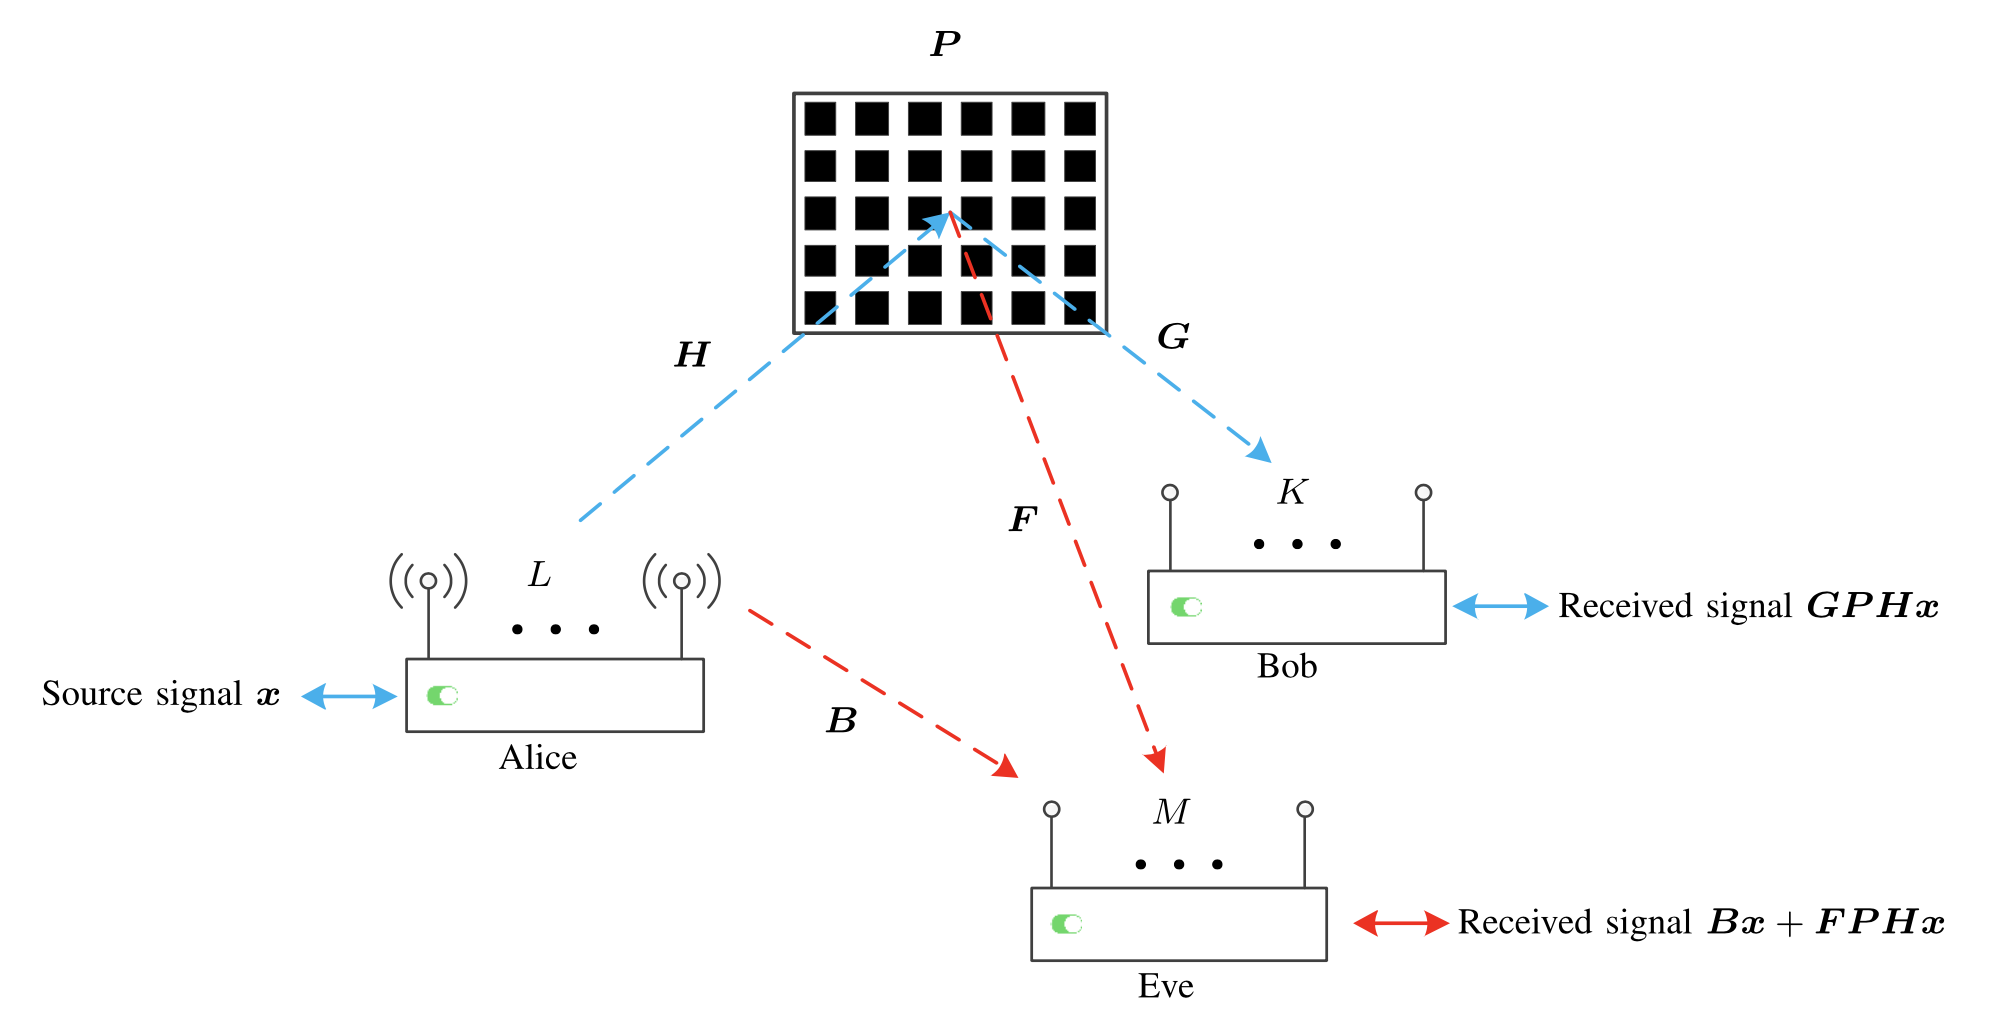
\includegraphics[width=\linewidth]{imgs/problem-description.png}
  \caption{Setup}
  \label{fig:correlation_sk}
\end{figure}

In \cite{9328149}, the authors studied how to use RISs to allow communications between two users without LOS, while making the signal undeciphrable for eavesdroppers. We call $L$ the transmitter's antennas, $K$ the receiver's antennas, $M$ the eavesdropper's antenna, and $N$ the RIS reflecting elements. We assume $L \ge K \ge 2$.

We define $\bm{H} \in \C^{NxL}$ the channel response \footnote{A channel response for a MIMO communication is a matrix made of complex number, where the position $i,j$ indicates the signal received from antenna $j$ to antenna $i$} from the transmitter to the RIS, $\bm{G} \in \C^{KxN}$ the channel response from the RIS to the receiver, $\bm{P} = diag\{p\} \in \C^{NxN}$ a diagonal matrix in which the $n$th diagonal element represents the reflection coefficient of the $n$th unit at the RIS.

The objective is making the receiver's final signal $GPH$ a diagonal matrix, while making every possible eavesdropper's final signal a full matrix.

We will leave for later the technical details of why this would achieve secrecy for the legitimate users or how the actors communicate with each others, and will just focus on the mathematics behind the calculation. It is possible to read more in the paper \textit{Space shift keying modulation for MIMO channels} \cite{5165332}, which we will summarize in a later chapter.

Our contribution to the field will be to generalize these calculations to $J$ receving users and $M$ RISs used in parallel and in sequence.

Formally, the condition we want to satisfy is:

\begin{equation}
  || [\bm{GPH}]_{:,1:K} - [[\bm{GPH}]_{:,1:K}]_{diag} || ^2 = 0
  \label{eq:diag_condition}
\end{equation}

Where $[GPH]_{:,1:K} \in \C^{KxK}$ denotes the first K columns of the matrix $\bm{GPH} \in \C^{KxL}$.

Given

\begin{equation}
  \bm{W} = \sum_{i,j = 1, i \ne j}^{K} (g_{j,:} \odot h_i^T)^H (g_{j,:} \odot h_i^T)
\end{equation}
\begin{equation}
  \rank(\bm{W}) = K(K-1)
\end{equation}
\begin{equation}
  \rank(\bm{W}) - \nullop(\bm{W}) = N
\end{equation}
Where $\nullop$ refers to the dimension of the $\nullop$ space.
\begin{equation}
  \nullop(\bm{W}) = N - (K^2 - K)
\end{equation}

The formula \eqref{eq:diag_condition} can be rewritten as

\begin{equation}Wp = 0\end{equation}

and the solutions of $p$ can be found in the $\nullop$ space of $\bm{W}$. Using singular value decomposition (SVD), we can decompose

\begin{equation}
  \bm{W} = \bm{R \Sigma V}^H \footnote{An hermitian transpose of $\bm{V}$ ($\bm{V}^H$), means we fist transpose the matrix ($\bm{V} \rightarrow \bm{V}^T$), then take the conjugate of every element (so invert the sign of the immaginary part).}
\end{equation}

With SVD, we have $\bm{\Sigma} = diag(\sigma) \in C^{NxN}$ a diagonal matrix. the first $\rank(\bm{W}) = K^2-K$ elements of $\sigma$ are non-zero, while the last $\nullop(\bm{W}) = N - (K^2-K)$ elements are zero \cite{svd}.

Given a more generic $\bm{A} \in \C^{mxn} = \bm{R}'\bm{ \Sigma}' \bm{V}'^H$, we have the column vectors of $R'$ being an orthonormal span of $C^m$, and the row vectors of $V'$ being an orthonormal span of $C^n$.

Suppose $\bm{A}$ is an Hermitian matrix (meaning $\bm{A} = \bm{A}^H$). This will be useful later, as $\bm{W}$ is also an Hermitian matrix by construction. Let's call $k$ the $\nullop$ space dimension of $\bm{A}$, and ,by the property above, the $\nullop$ space dimension of $\bm{A}^H$ too.

The last $k$ columns of $\bm{R}'$ are a span of the $\nullop$ space
\begin{equation}
  N(\bm{A}^H) = [r_{m-k}, ..., r_m ] \in \C^{mxk}
\end{equation}
while the last $k$ rows of $V'^H$ are a span of the $\nullop$ space
\begin{equation}
  N(\bm{A}) = \begin{bmatrix} v'^H_{n-k} \\ ... \\ v'^H_n \end{bmatrix} \in \C^{kxn}
\end{equation}
Being $\bm{A}$ an Hermitian matrix, the two $\nullop$ spaces are both solutions to $\bm{A}x = 0$.

Consider now $\bm{W} \in C^{NxN}$. The paper in question uses equation (7) to find the solutions, since $W$ is hermitian and square. Taken $\bm{U} \in \C ^ {Nx(N-(K^2 - K))}$ the last $N-(K^2 - K)$ columns of the left singular matrix $\bm{R}$. $\bm{U} \in \bm{N}(\bm{W})$ for the explanation above. We then have

\begin{equation}\bm{WU} = 0\end{equation}
\begin{equation}p = \bm{U}q\end{equation}
\begin{equation}\bm{WU}q = 0\end{equation}

being true, and $q \in \C^{N-(K^2 - K)}$ can be a random vector.

\section{Understanding signal decyphering}
How can the actors communicate, if the result is a diagonal matrix with random value?

\subsection{Space Shift Keying Modulation
}

We will use a technique called \textit{Space Shift Keying} (SSK) Modulation \cite{5165332}, where \textit{antenna indices are used as the only means to relay information}. Given $K$ the number of antenna of the actors in the system, we can send $log_2(K)$ bits by mapping each combination of bits to a specific antenna.
\footnote{This may seem rather unoptimized, as we use only one antenna instead of combinations of them. To see a more general approach, the authors also wrote the paper \cite{4699782}, where they discuss a more general approach using multiple active antennas at the same time. The general approach will also work with our proposed solution.}

\begin{figure}[H]
  \centering
  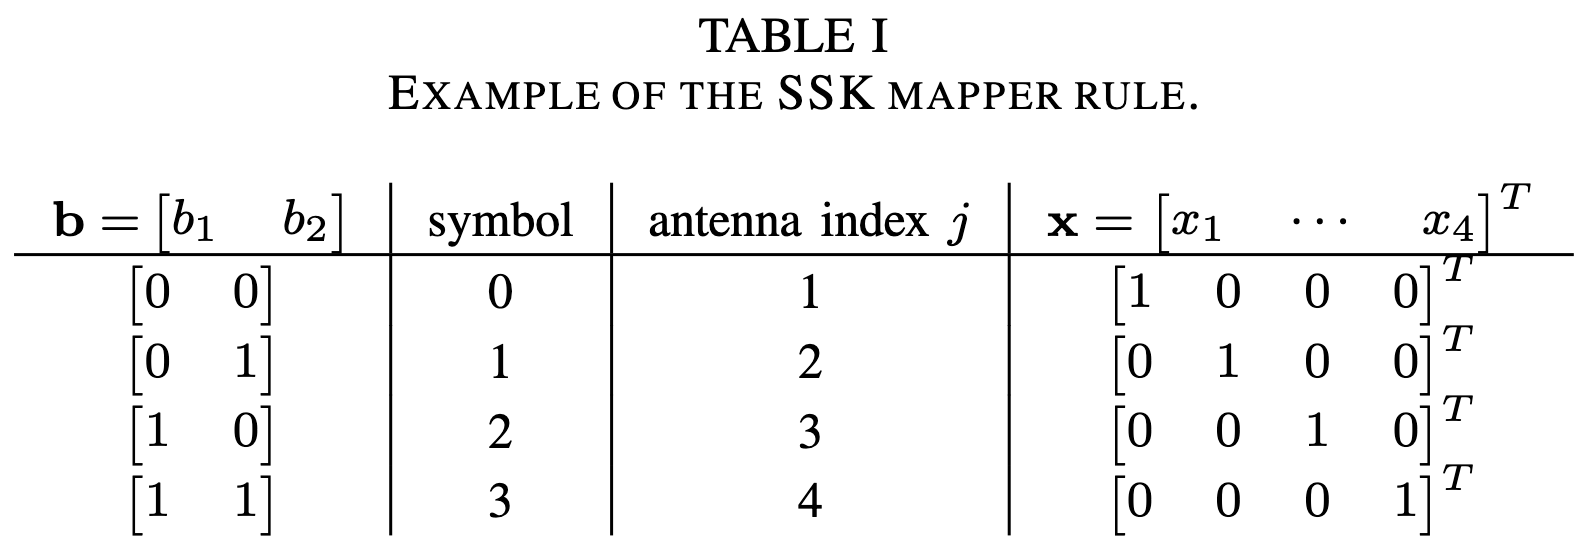
\includegraphics[width=\linewidth]{imgs/ssk_conversion_table.png}
  \caption{SSK conversion table, from \cite{5165332}}
  \label{fig:ssk_conversion_table}
\end{figure}

\subsubsection{Direct Detection}
Given a channel gain matrix $\bm{B} \in \C^{KxK}$ and the input vector $x \in \C^K$ with only one element equal to $1$, the signal received is
\begin{equation}
  y = \bm{B}x + \sigma^2
\end{equation}
To understand the antenna index which sent the message, we need to find the column $b_j$ which is most similar to $y$.

\begin{equation}
  j = \argmax_j\ p_y (y | x_j, \bm{B}) = \argmin_j\ || y - b_j ||^2
  \label{eq:direct_detection}
\end{equation}

\subsubsection{Diagonalized Reflection Detection}
Following \cite{9328149}, for a reflected signal we have
\begin{equation}
  y = \bm{GPH}x + \sigma^2
\end{equation}
Given that $\bm{GPH}$ is a diagonal matrix and $x$ has only one element equal to $1$, the resulting vector $\bm{GPH}x$ will still be a vector with only one element non zero. Adding noise, to find the antenna index we search for the biggest value in the vector.

\begin{equation}
  j = \argmax_j\ y_j
  \label{eq:reflection_detection}
\end{equation}
\newpage
\subsection{Cascaded Channel Estimation}
To understand how the actors (and in particular the RISs controller) estimate the channel gain between them, we redirect to the paper \textit{Cascaded Channel Estimation for Large Intelligent Metasurface Assisted Massive MIMO} \cite{8879620}. While we will not summarize the content here, we will still give a general idea of how to use the algorithm in the paper to estimate $\bm{G}$ and $\bm{H}$.
\begin{itemize}
  \item The transmitter comunicates to the RIS controller a setup message $x'$ that it will send to the receiver;
  \item The RIS will set a random $\bm{P}'$; % \footnote{As discussed before, in case of multiple RIS in series we set all of them randomly. Later, we setup just the last $P_M$ correctly based on $G'$ and $H$ estimations.}
  \item The receiver gets a signal $y'$ (which will mean nothing), and sends it back to the RIS controller;
  \item Based on $x', y', \bm{P}'$ the RIS controller estimates $\bm{G}, \bm{H}$ and correctly setup $\bm{P}$;
  \item The transmitter sends $x$, and the receiver gets $y$ which can correctly convert back;
  \item If transmitter and receiver are moving, the procedure will start all over. Otherwise, $\bm{G}$ and $\bm{H}$ remain the same, and the RIS controller can just create a new $\bm{P}$ for the next messages.
\end{itemize}

\section{Physical Layer Security in reflected signals towards multiple receivers}

In real life scenarios, we deal with more than two communicating actors. We want to expand the work of chapter 3 by having it support multiple RISs in series and multiple receivers from the same transmitter. Once we have those, we can generalize it to also have receivers getting signals from multiple independent reflections of RISs.

We will first, however, make some simplifications about the actors by having $L = K$ for all of them\footnote{We want the actors to be able to communicate with each other. Since the transmitter needs to have an equal or greater number of antennas than the receiver, but the roles may later switch, it follows that the number of antennas must be equal for the calculation. Using more antennas can still be done, by not considering the values coming from them (like the original paper did as well).}. We will still consider one transmitter, with $J \ge 1$ receivers.

In this section, we consider the scenario illustrated in \cref{fig:correlation_sk2}, where a single transmitter Alice and multiple receivers exist. Frank is a direct receiver in line of sight. Bob and Charlie receive the signal from two double RIS reflections. Eve receives both the direct signal and the reflecting signal from all RISs. \footnote{It should be noted that if \textit{Eve} is in the same position as \textit{Frank} and receives just the direct signal, our particular framework would not give us physical layer security, and higher layer security would be needed. If instead \textit{Eve} has no line of sight, the message would be completely unreadable from the start, since it would receive random matrices.}

\begin{figure}[H]
  \centering
  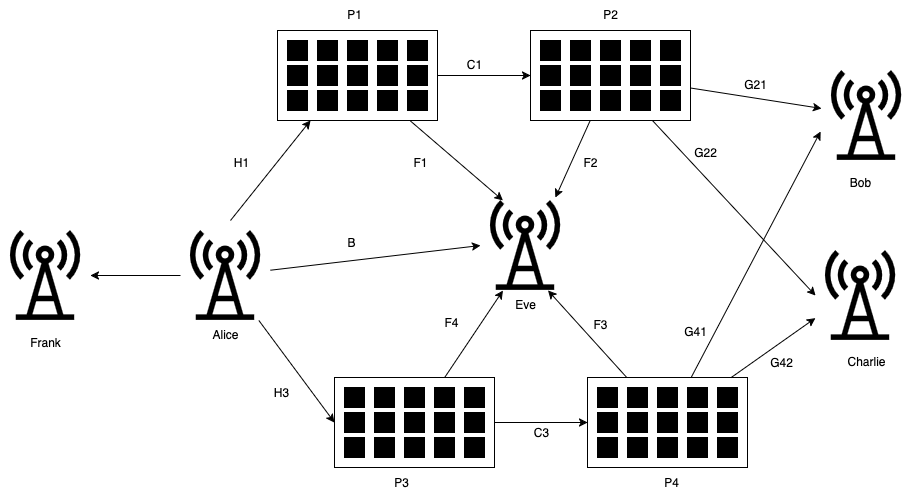
\includegraphics[width=\linewidth]{imgs/complex-situation.png}
  \caption{Complex setup for secure message transmission}
  \label{fig:correlation_sk2}
\end{figure}

More generally, we would have $M$ consecutive RIS (in series) that reflect a signal, $J$ legitimate receivers and $Q$ different paths of RIS (in parallel) to send the signal at the same time. \footnote{The paths could have a different number of RIS (for example, a path of three and another of two). The results would still hold.}

\subsection{Reflecting to multiple users}

We consider the case where the transmitter wants to send the signal to $J$ receivers without LOS. We define the link from the RIS to the receiver $j$ as $\bm{G}_j$. The condition we want to satisfy is

\begin{equation}
  \forall j \in \{1, 2, \ldots , J\} \rightarrow || \bm{G}_j\bm{PH} - [\bm{G}_j\bm{PH}]_{diag} || ^2 = 0
\end{equation}

\begin{equation}
  \forall j \in \{1, 2, \ldots , J\} \rightarrow \bm{W}_j = \sum_{i,k = 1, i \ne k}^{K} (g_{j_{k,:}} \odot h_i^T)^H (g_{j_{k,:}} \odot h_i^T)
\end{equation}

\begin{equation}
  \forall j \in \{1, 2, \ldots , J\} \rightarrow \bm{W}_j p = 0
\end{equation}

\begin{equation}
  \begin{bmatrix}
    \bm{W}_1  \\
    \bm{W}_ 2 \\
    ...       \\
    \bm{W}_J
  \end{bmatrix}
  p = 0
\end{equation}

\begin{equation}
  \begin{bmatrix}
    \bm{W}_1  \\
    \bm{W}_ 2 \\
    ...       \\
    \bm{W}_J
  \end{bmatrix}
  = \bm{W} \in \C ^ {JNxN}, \bm{W} = \bm{R \Sigma V}^H
\end{equation}

The problem we have now is that $\bm{W}$ is not a square matrix anymore, so we cannot use the last $N - (K^2 - K)$ columns of $\bm{R}$ to calculate the $\nullop$ space and $p$ with its linear combination, by using formula \eqref{null-space-hermitian}. The $\nullop$ space would have dimension $N(\bm{W}) \in \C^{JN x (N - (K^2 - K))}$, but that would require a $p \in C^{JN}$ instead of $p \in C^{N}$.

We can, however, use the last $N - (K^2 - K)$ rows of $\bm{V}^H$, then apply again the hermitian transposition to get our desired solution. Remember that $N(\bm{W})$ can also be calculated using the left singular matrix, by using formula \eqref{null-space-normal}. $\bm{W}$ is not a square matrix, so $\bm{W} \ne \bm{W}^H$,

\begin{equation}
  N(\bm{W}) = \begin{bmatrix} v^H_{N - J(K^2 - K)} \\ ... \\ v^H_N \end{bmatrix} ^ H
\end{equation}

Take $\bm{U}_1 \in \C ^ {N - J(K^2 - K) \times N}$ the last $N - (K^2 - K)$ rows of $\bm{V}^H$, and
\begin{equation}
  \bm{U} = \bm{U}_1^H \in \C ^ {N x N - J(K^2 - K)}
\end{equation}

We now can apply the same method as before

\begin{equation}p = \bm{U}q\end{equation}

\begin{equation}\bm{WU} = 0\end{equation}

\begin{equation}\bm{WU}q = 0\end{equation}

\subsection{RISs in parallel}

Given the previous property, it follows that we can use $Q$ independent RISs, each one reflecting the signal to $J$ multiple receivers, and without LOS from each other. For the receiver $j \in \{1, 2, \ldots , J\}$, we have

\begin{equation}
  \sum_{m=1}^M \bm{G}_j \bm{P}_m \bm{H}_m x = (\sum_{m=1}^M \bm{G}_j \bm{P}_m \bm{H}_m) x
\end{equation}

The sum of diagonal matrices is still a diagonal matrix, so the property still holds. Remember that we only care about the indexes of the active antennas and not their values, so there is no problem in adding them together.

\subsection{RISs in series}

We consider the case where the signal is bounced between $M$ RISs with reflection matrixes $\bm{P}_1, \ldots, \bm{P}_m$ in this way:

\begin{equation}
  \text{Transmitter} \rightarrow \text{RIS 1} \rightarrow ... \rightarrow \text{RIS M} \rightarrow \text{Receiver}
\end{equation}

We call $\bm{C}_i \in \C^{N \times N}$ the channel gain between $\bm{P}_i$ and $\bm{P}_{i+1}$. We need to solve

\begin{equation}
  || \bm{GP}_1\bm{C}_1...\bm{P}_M\bm{H} - [\bm{GP}_1\bm{C}_1...\bm{P}_M\bm{H}]_{diag} || ^2 = 0
\end{equation}

We can generate $p_1, ..., p_{M-1}$ as random reflections, and calculate the last one based on the previous. An advantage we get is that eavesdroppers listening from a middle RIS will not be able to decipher the signal either.

Given $r_i \in [0, 1]$ the absorption coefficient, and $\theta_i \in [0, 2\pi]$ the phase shift, we can choose them randomly for all RIS $p_m$ vectors, but the last one.

\begin{equation}
  \forall m \in [1, M-1] : p_m[i] = \eta \cdot r_i \cdot e^{j\theta_i}
\end{equation}

Given now

\begin{equation}
  \bm{G}' = \bm{GP}_1\bm{C}_1...\bm{P}_{M-1}\bm{C}_{M-1} \in \C^{K \times N}
\end{equation}

We can consider now the problem of solving

\begin{equation}
  || \bm{G}'\bm{P}_M\bm{H} - [\bm{G}'\bm{P}_M\bm{H}]_{diag} || ^2 = 0
\end{equation}

Which can be solved as before.
\footnote{It is also possible to set up randomly the last $M-1$ RIS and calculate the first one using $\bm{G}$ and $\bm{H}'=\bm{C}_1\bm{P}_2\bm{C}_2...\bm{P}_M$. The properties still hold.}
\footnote{Estimating the channel gains $\bm{G}$ and $\bm{H}$, based on \cite{8879620}, could be more difficult, given that we do not have full control on $\bm{P}=\bm{P}_1\bm{C}_1...\bm{P}_M$ anymore. We can however estimate directly $G'$ by keeping the same random $\bm{P}_1, ..., \bm{P}_{M-1}$ in both the acknowledgment round and the message transmission round, and just modify $\bm{P}_M$ after estimating $\bm{G}'$ and $\bm{H}$ to correctly deliver the message.}

If we have multiple $\bm{G}_j$, it will be enough to calculate all the $\bm{G}'_j$ and proceed as before, allowing us to combine these properties in more complicated scenarios.

\subsection{Complex reflections}

The receiver could also get the signal from all the RISs in series, if in the right position.

For example, let's say it receives the signals $\bm{GP}_1\bm{H}_1x$ and $GP_1C_1P_2H_2x$. To solve this system, instead of setting $\bm{P}_1$ randomly, we would need first to solve it using $\bm{G}$ and $\bm{H}_1$, then solve $\bm{P}_2$ using $\bm{G}'=\bm{GP}_1\bm{C}_1$ and $\bm{H}_2$. The sum of the two signals would still be readable for the receiver correctly.

While the calculations of $\bm{P}_1$ depend on $\bm{G}$ and $\bm{H}_1$, the signal would still be random and undecipherable for an eavesdropper receiving it.

\section{Simulation Results}

In this chapter, we will evaluate the performance of the proposed framework through extensive simulations of different scopes and scenarios.

In section 5.1, we perform Bit Error Rate (BER) analysis using stochastic simulations to show the relation between correct capture of the signal depending on the Signal to Noise Ratio (SNR). This will allow a direct comparison to the results obtained from the paper \cite{9328149}, to show the efficacy of our expansion.

In section 5.2, we will simulate more realistic scenarios by considering path loss and spatial deployment, creating BER heatmaps to show the validity of the framework in physical environments and the security offered for all possible locations of an eavesdropper.

\subsection{BER stochastic simulation}

We will show simulation results for different combinations of $M$ RISs and $J$ receivers, both with a single and double reflection paths from the trasmitter. In all scenarios, $K = 2, N = 16, \eta = 0.9$ will be the number of antennas for all actors, the number of reflecting surfaces and the reflection coefficients. We take these parameters to compare the results to the original paper \cite{9328149} \ref{fig:og_ber_sim}.

The direct link and the eavesdropper will try to understand the message by following the equation \eqref{eq:direct_detection}, while the receivers will try to understand it by following the equation \eqref{eq:reflection_detection}.

\subsubsection{Single RIS reflection (M=1)}

% \begin{figure}[H]
%   \centering
%   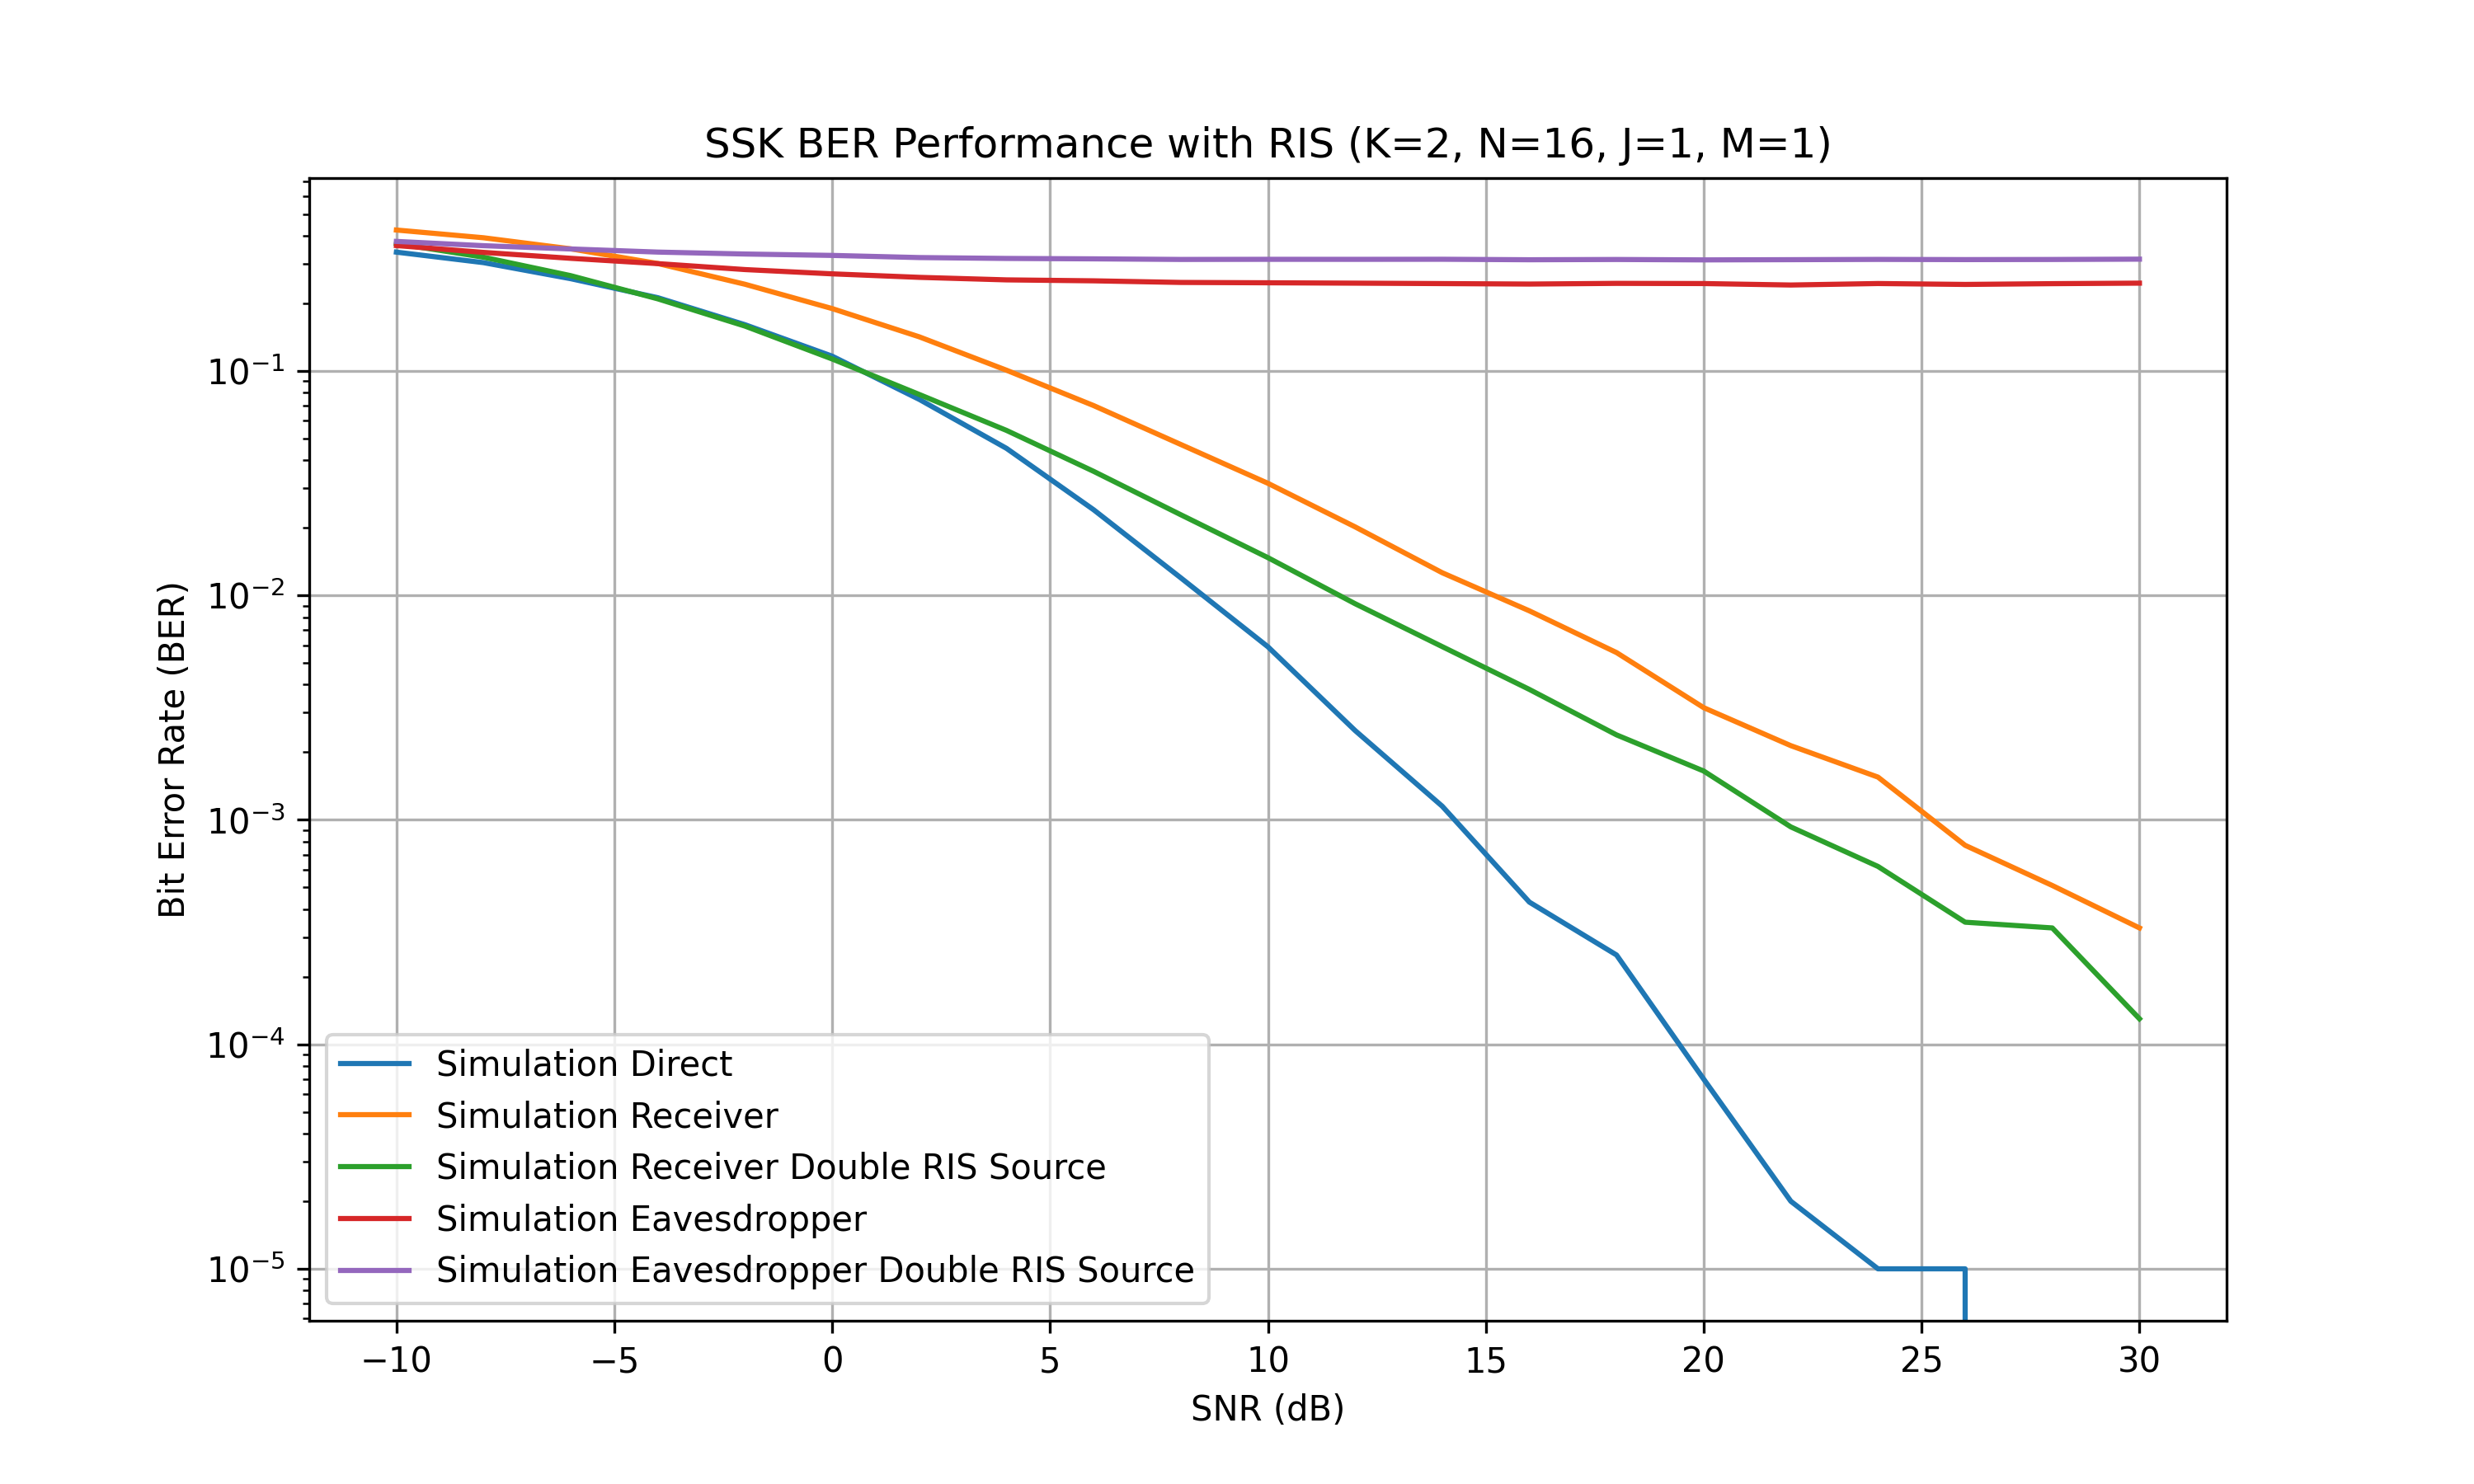
\includegraphics[width=0.9\linewidth]{imgs/ber-simulations/SSK BER Performance with RIS (K=2, N=16, J=1, M=1).png}
%   \caption{SSK BER Performance with RIS (K=2, N=16, J=1, M=1)}
%   \label{fig:simulation_j1_m1}
% \end{figure}

% \begin{figure}
%   \centering
%   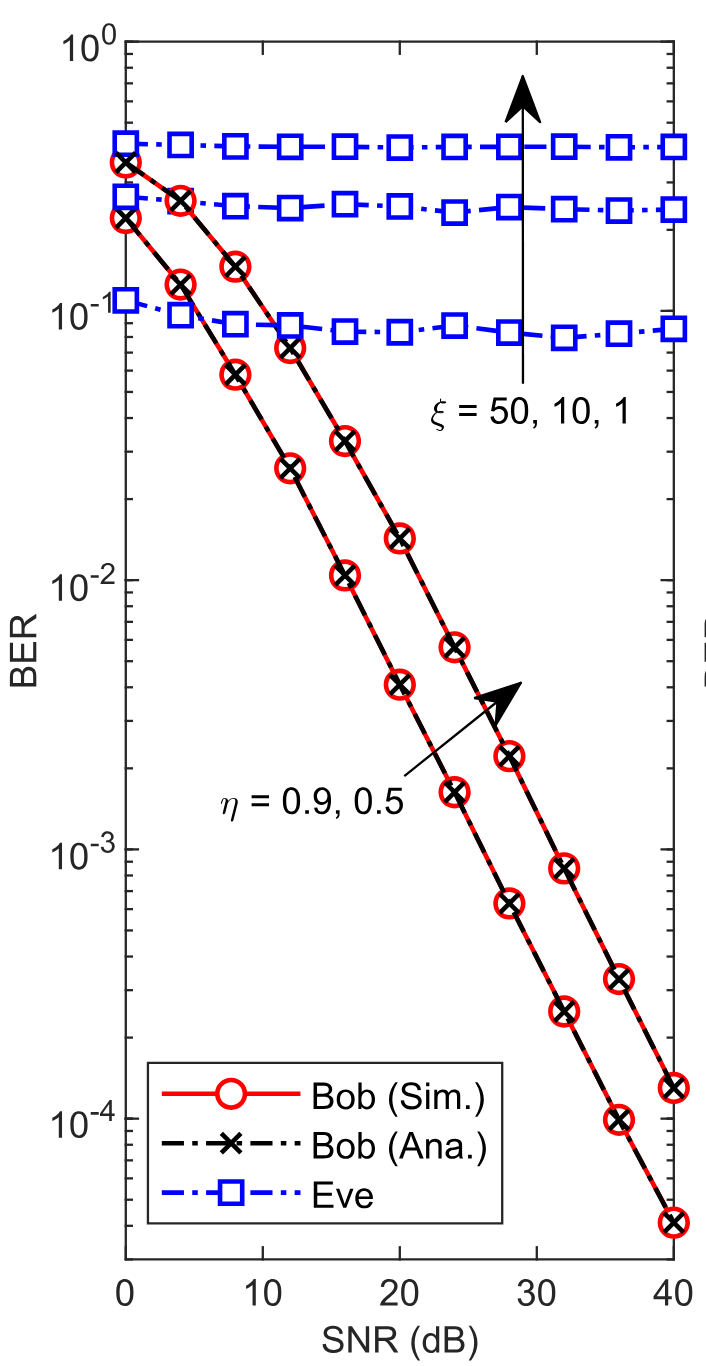
\includegraphics[width=0.2\linewidth]{imgs/og_ber_simulation.png}
%   \caption{Original BER analysis in \cite{9328149} for SSK scheme}
%   \label{fig:og_ber_sim}
% \end{figure}

\begin{figure}[H]
  \centering
  \begin{subfigure}[b]{0.76\textwidth}
    \centering
    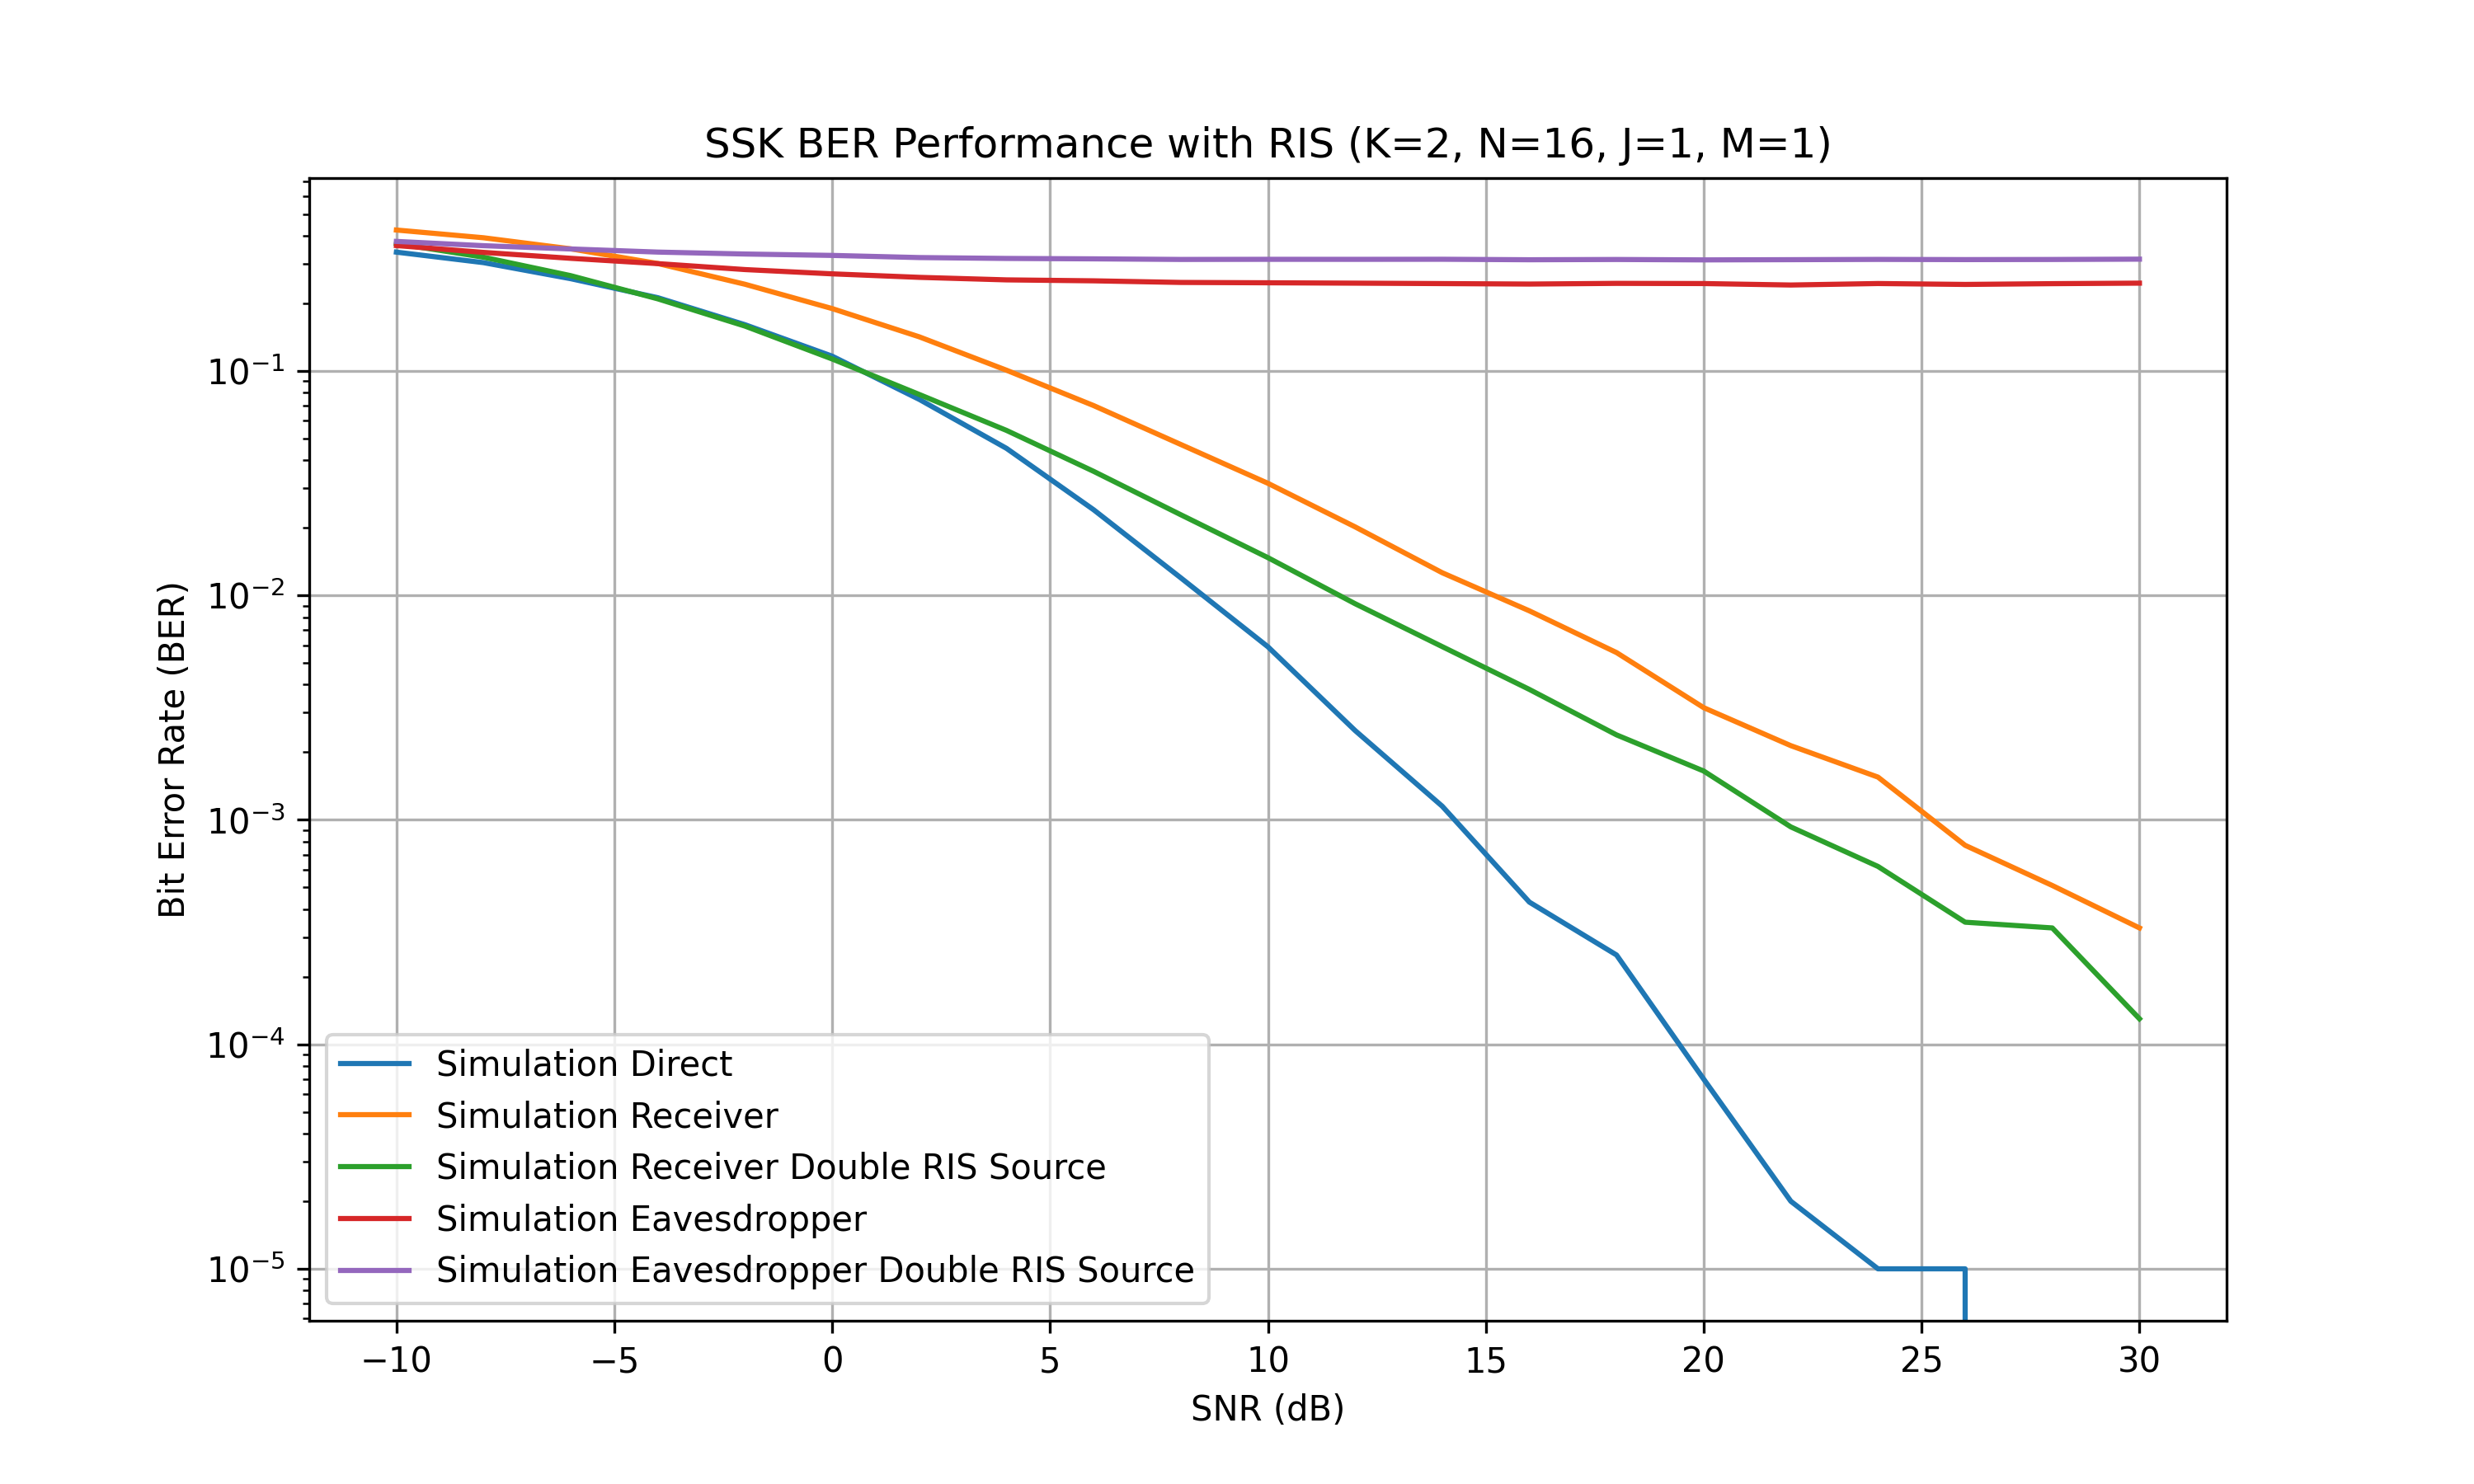
\includegraphics[width=\textwidth]{imgs/ber-simulations/SSK BER Performance with RIS (K=2, N=16, J=1, M=1).png}
    \caption{Our BER analysis}
    \label{fig:simulation_j1_m1}
  \end{subfigure}
  \hfill
  \begin{subfigure}[b]{0.23\textwidth}
    \centering
    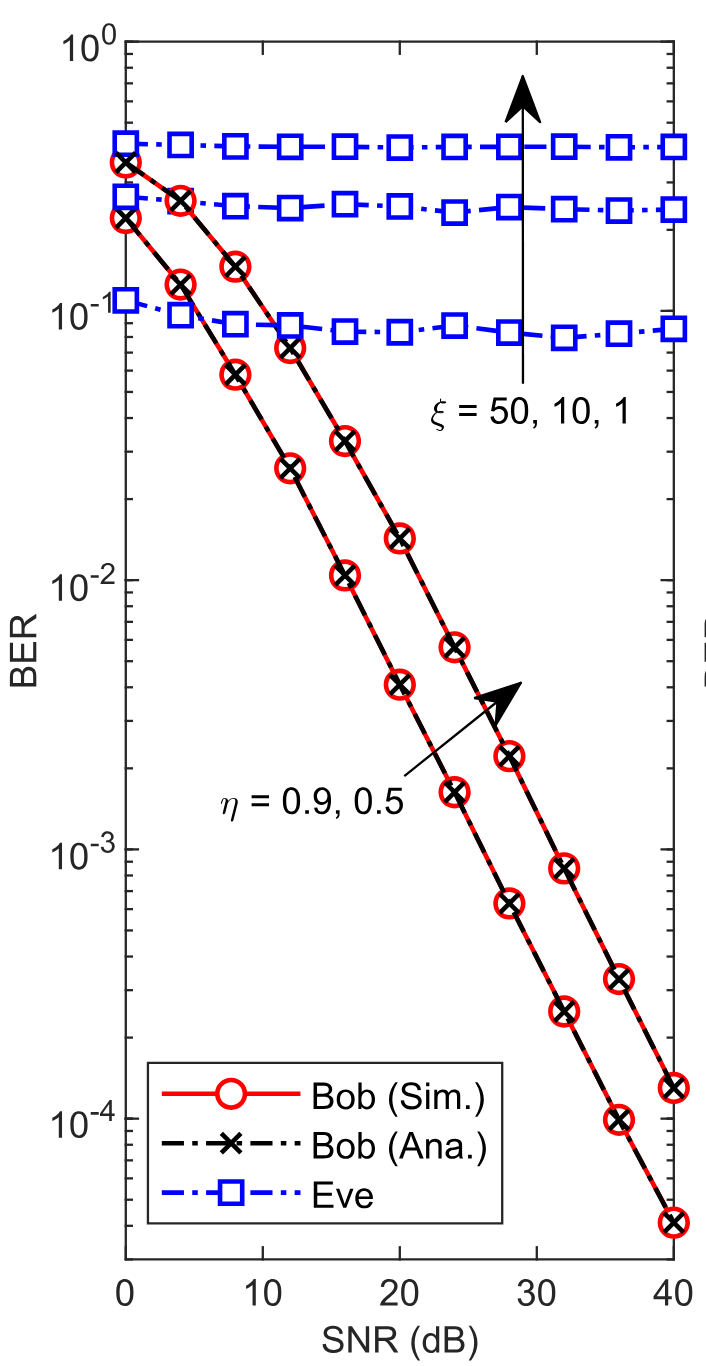
\includegraphics[width=\textwidth]{imgs/og_ber_simulation.png}
    \caption{\cite{9328149} BER analysis}
    \label{fig:og_ber_sim}
  \end{subfigure}
  \caption{SSK BER Performance with RIS (K=2, N=16, J=1, M=1)}
\end{figure}

We can see in ($M=1, J=1$) the results match with \cite{9328149}, for both \textit{Simulation Receiver} and \textit{Simulation Eavesdropper}.
\textit{Simulation Direct} is the strongest possible path, mainly because of the reflection loss due to $\eta$.
Combining two different RIS in parallel (\textit{Double RIS Source}) gives better signal to the receiver, while disturbing more the signal to the eavesdropper.

\begin{figure}[H]
  \centering
  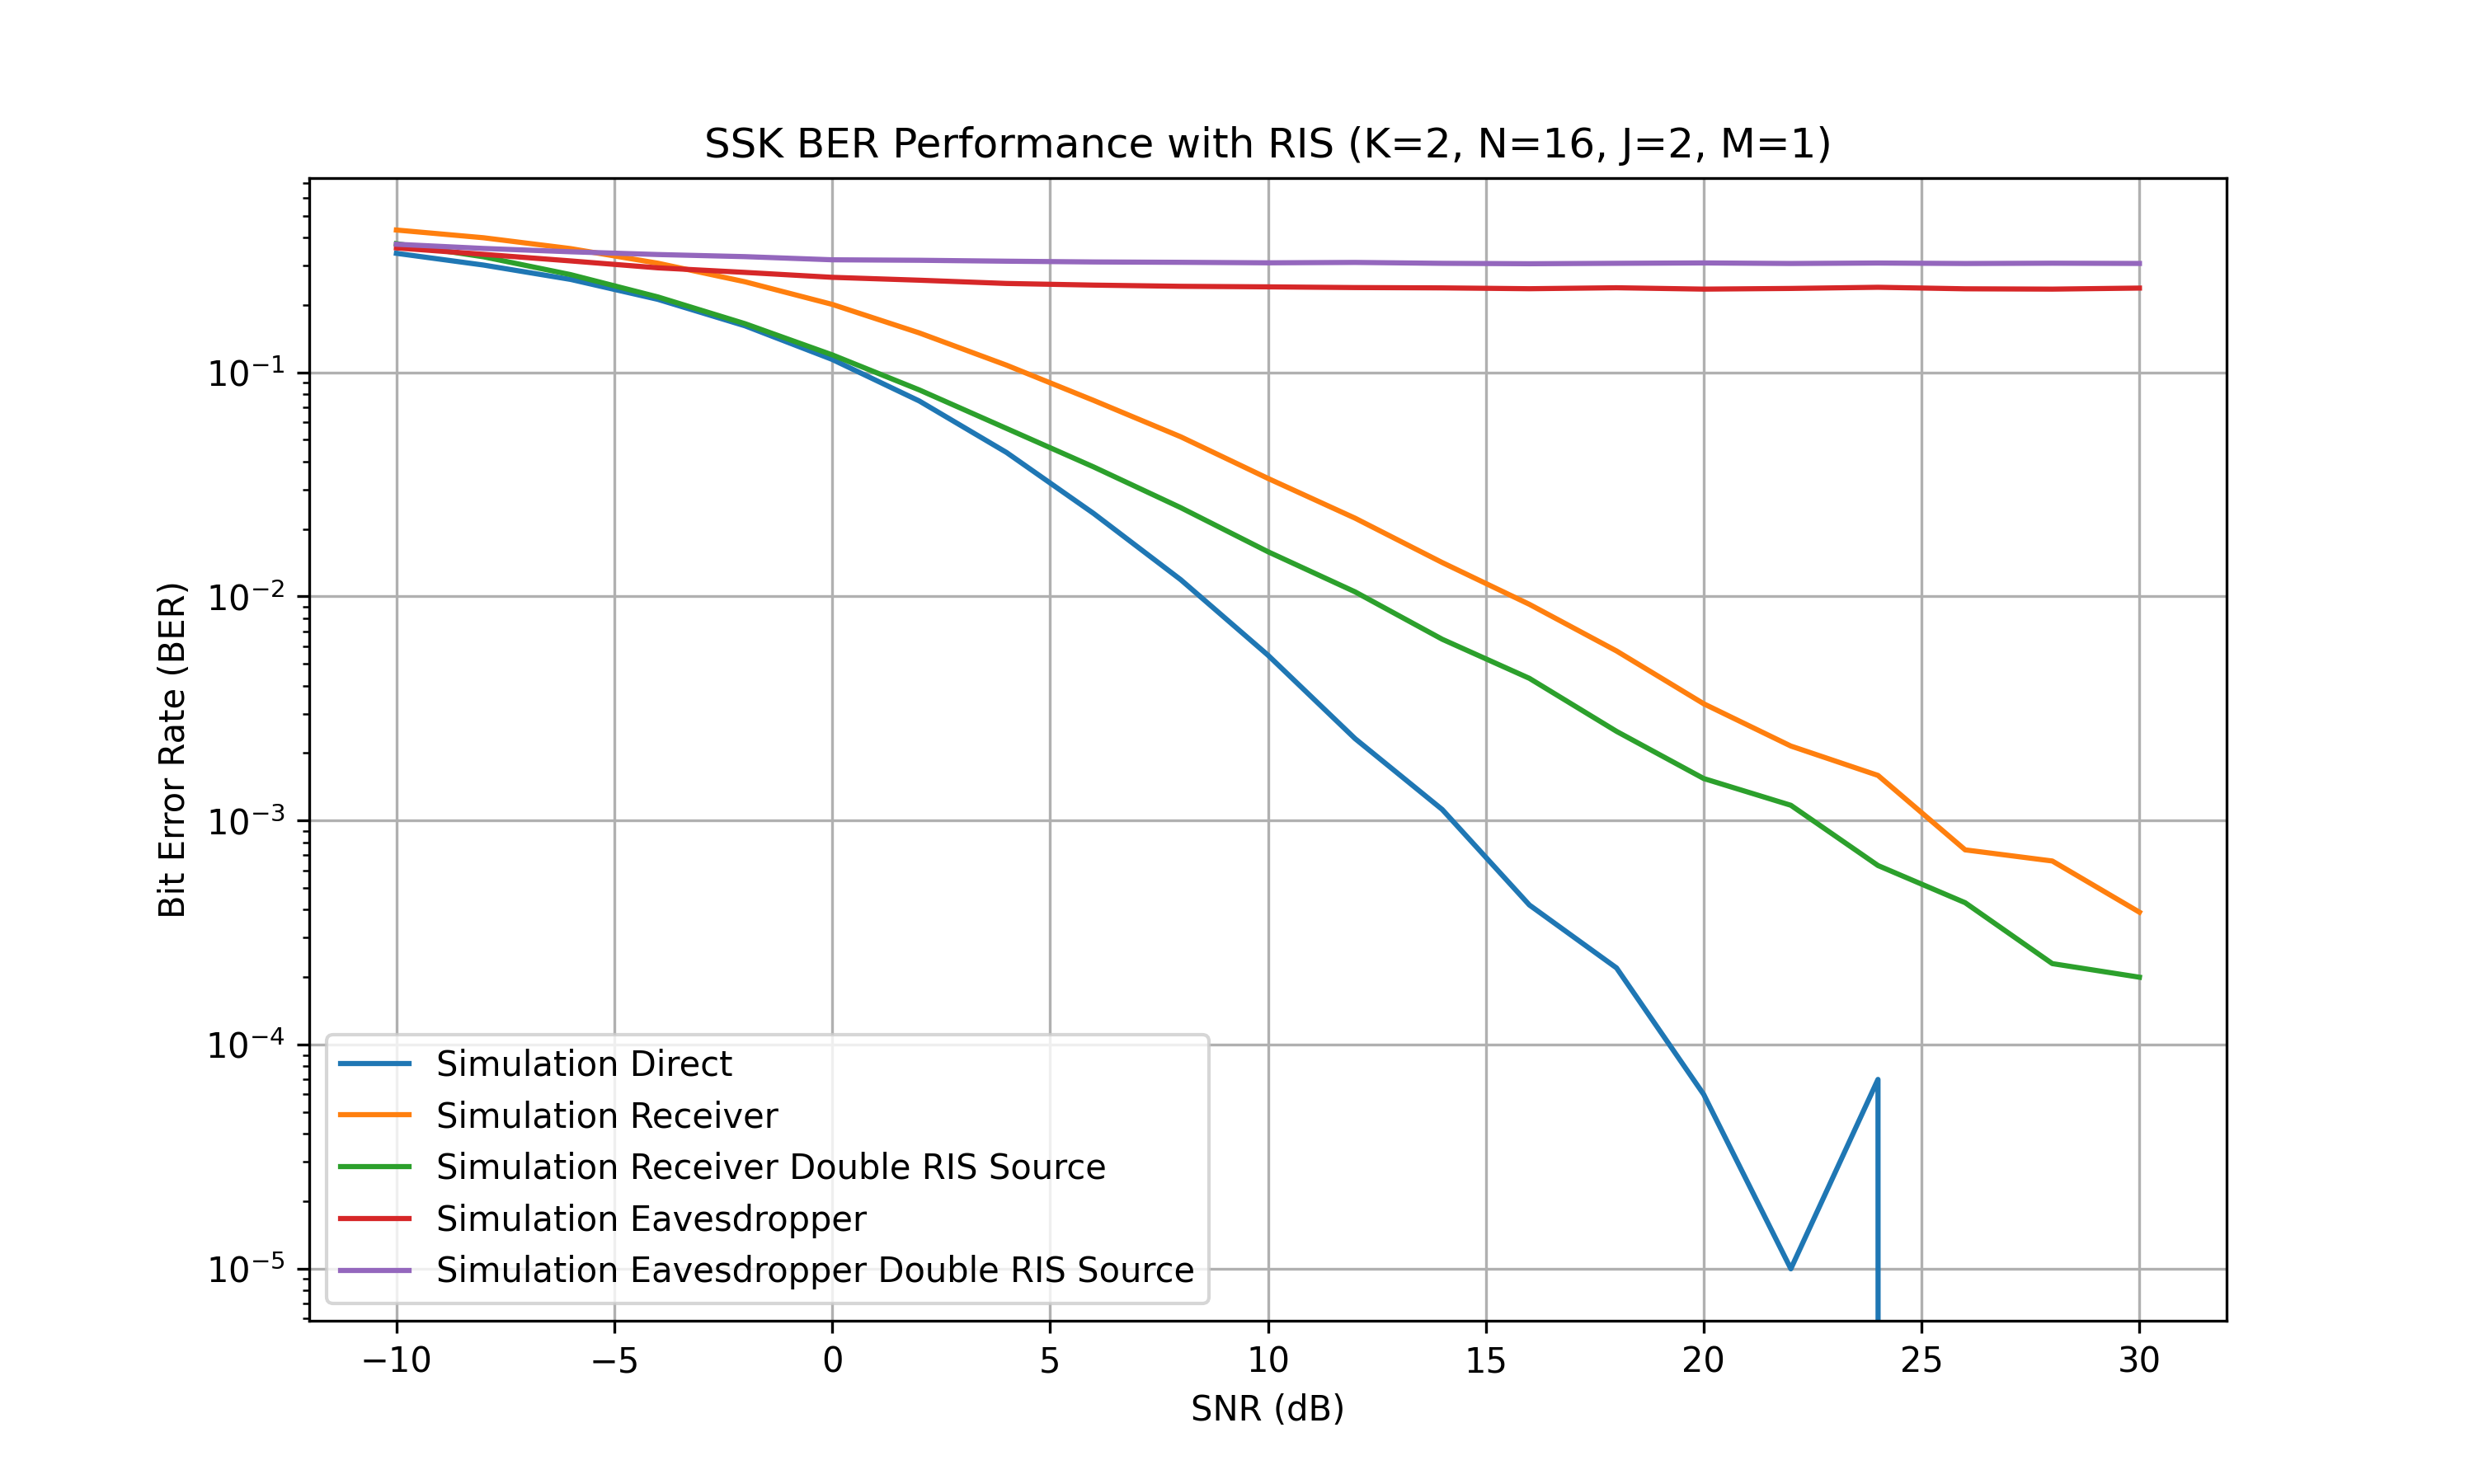
\includegraphics[width=0.9\linewidth]{imgs/ber-simulations/SSK BER Performance with RIS (K=2, N=16, J=2, M=1).png}
  \caption{SSK BER Performance with RIS (K=2, N=16, J=2, M=1)}
  \label{fig:simulation_j2_m1}
\end{figure}

Increasing the number of receivers does not influence the result of our framework: the receivers still get a good signal depending on the SNR, while the eavesdropper is not getting an advantage in understanding the message.

\subsubsection{Double RIS reflection (M=2)}

\begin{figure}[H]
  \centering
  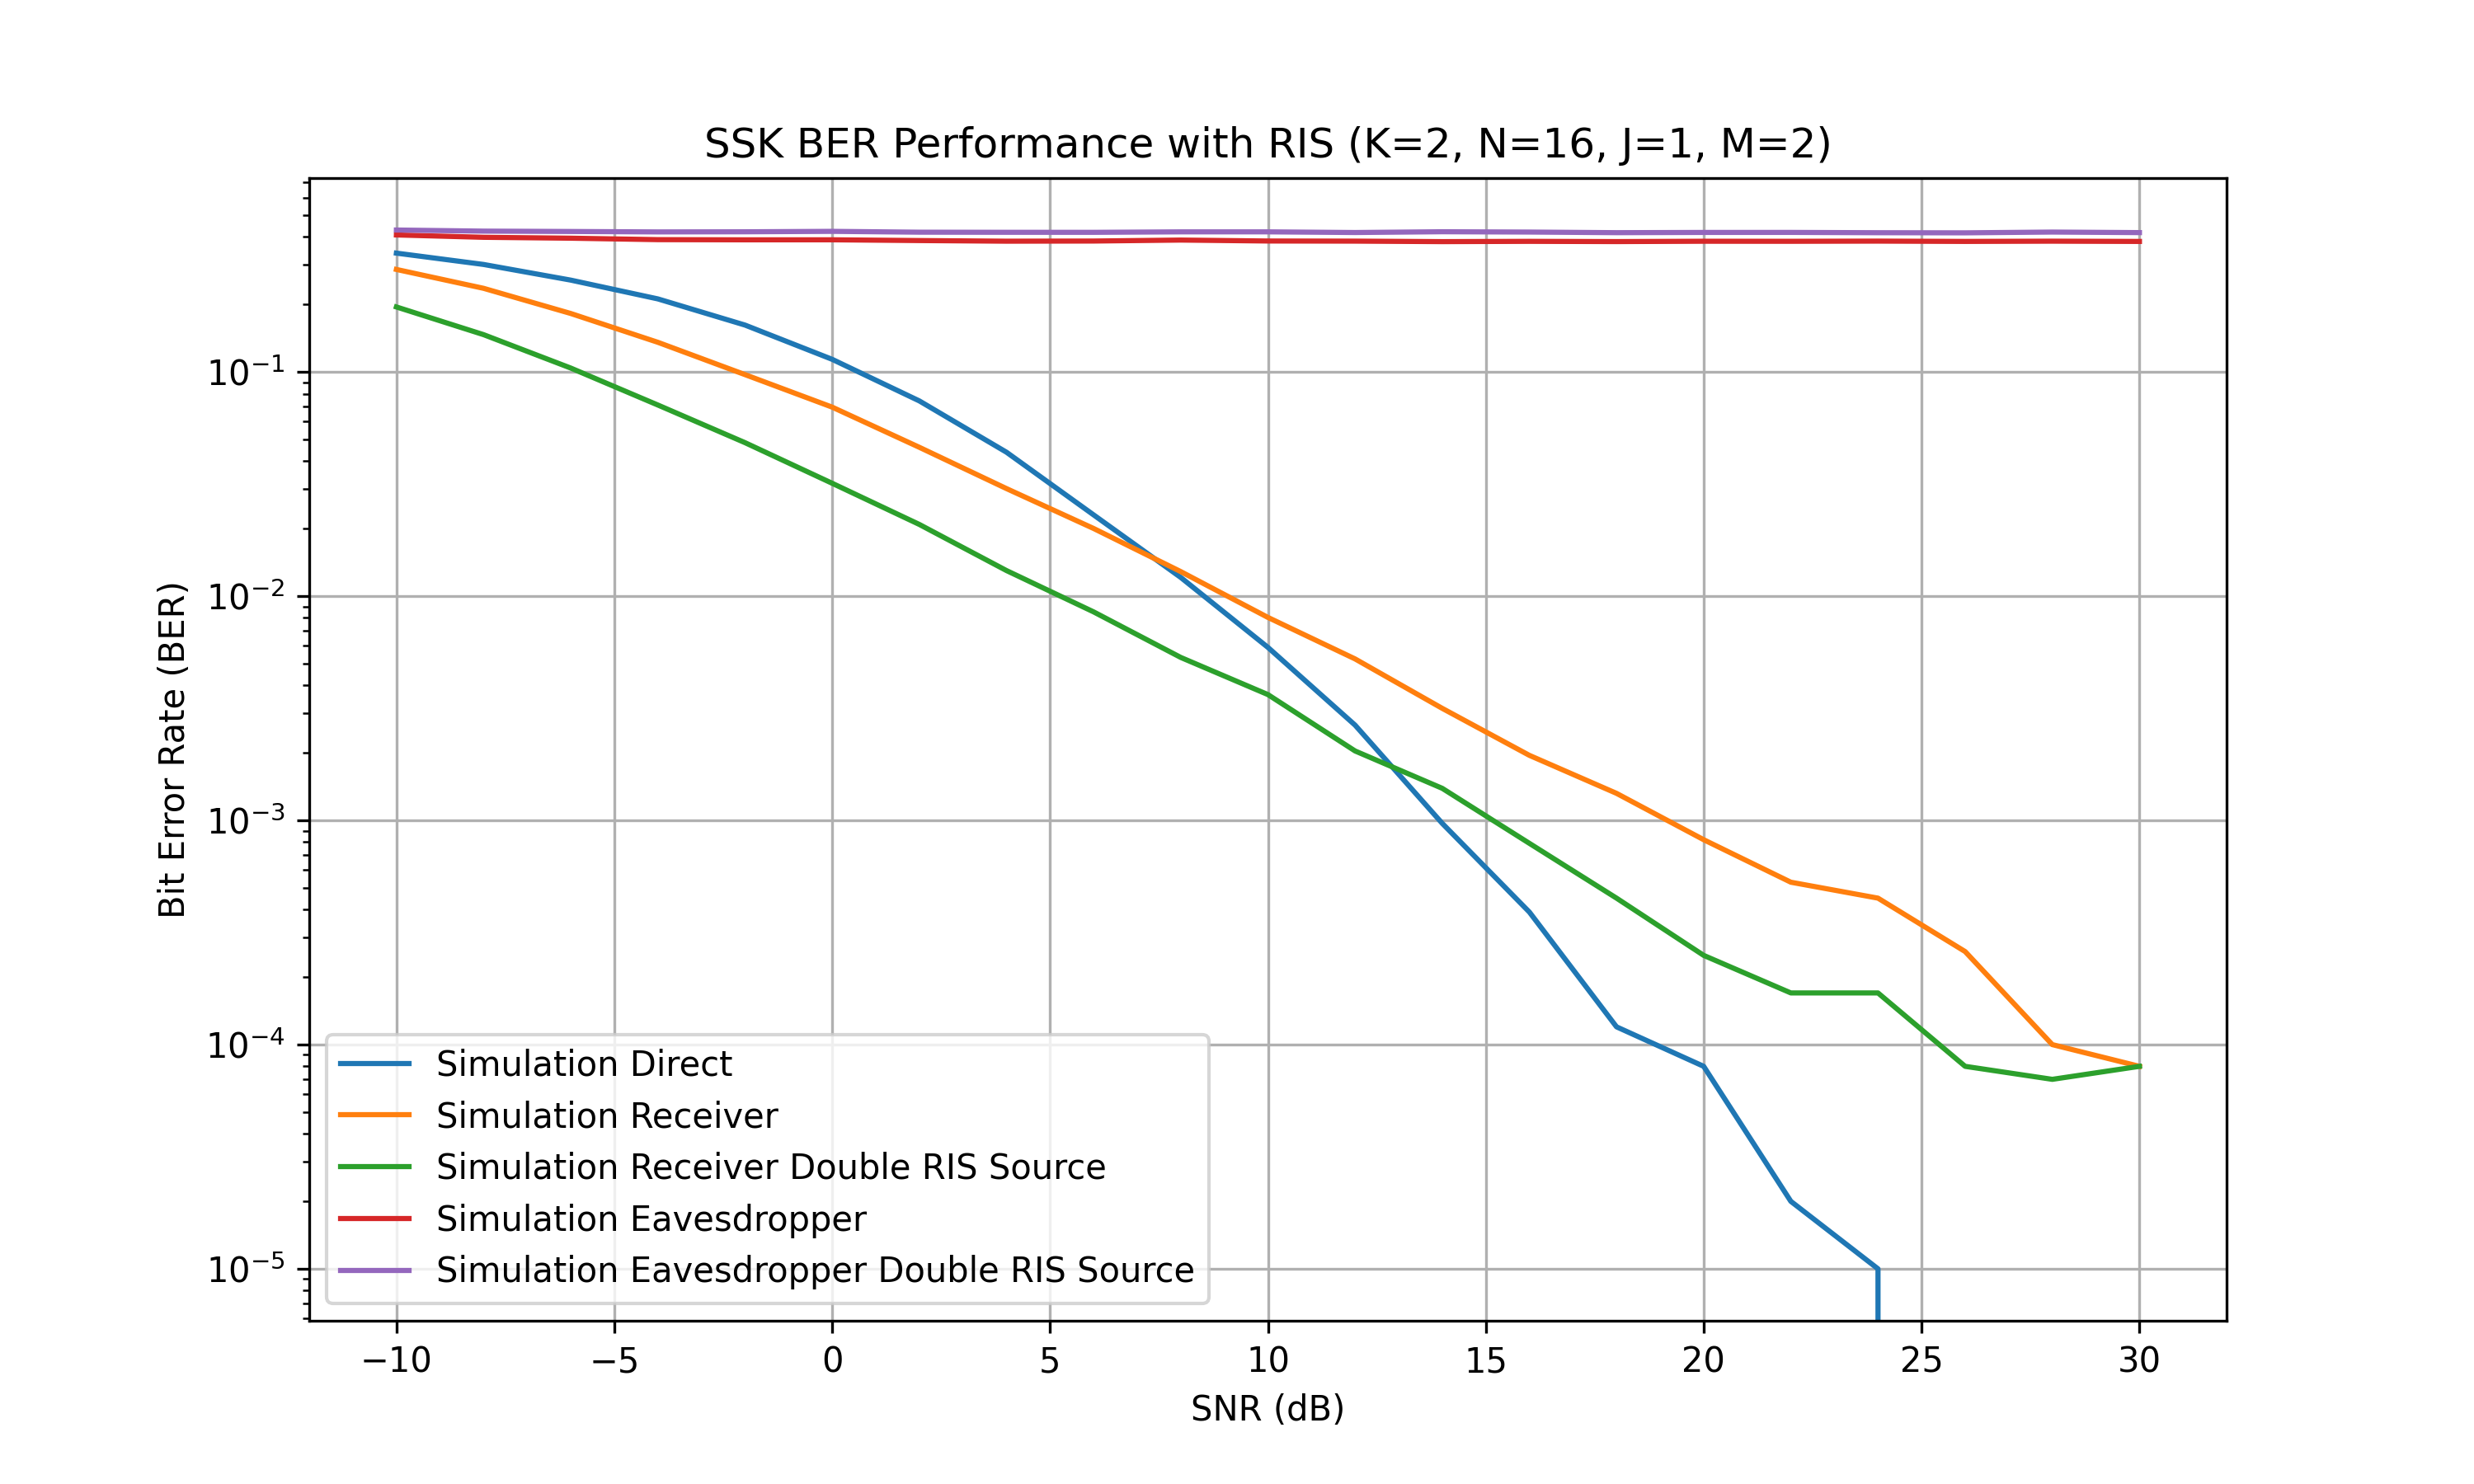
\includegraphics[width=0.9\linewidth]{imgs/ber-simulations/SSK BER Performance with RIS (K=2, N=16, J=1, M=2).png}
  \caption{SSK BER Performance with RIS (K=2, N=16, J=1, M=2)}
  \label{fig:simulation_j1_m2}
\end{figure}

With multiple RIS in series, the eavesdropper get a worse signal because of the double interference of the 2 RIS.
% \textbf{(TODO: Why the receiver is getting a better signal? Should it not be worse? Check normalization of the signal)}

\begin{figure}[H]
  \centering
  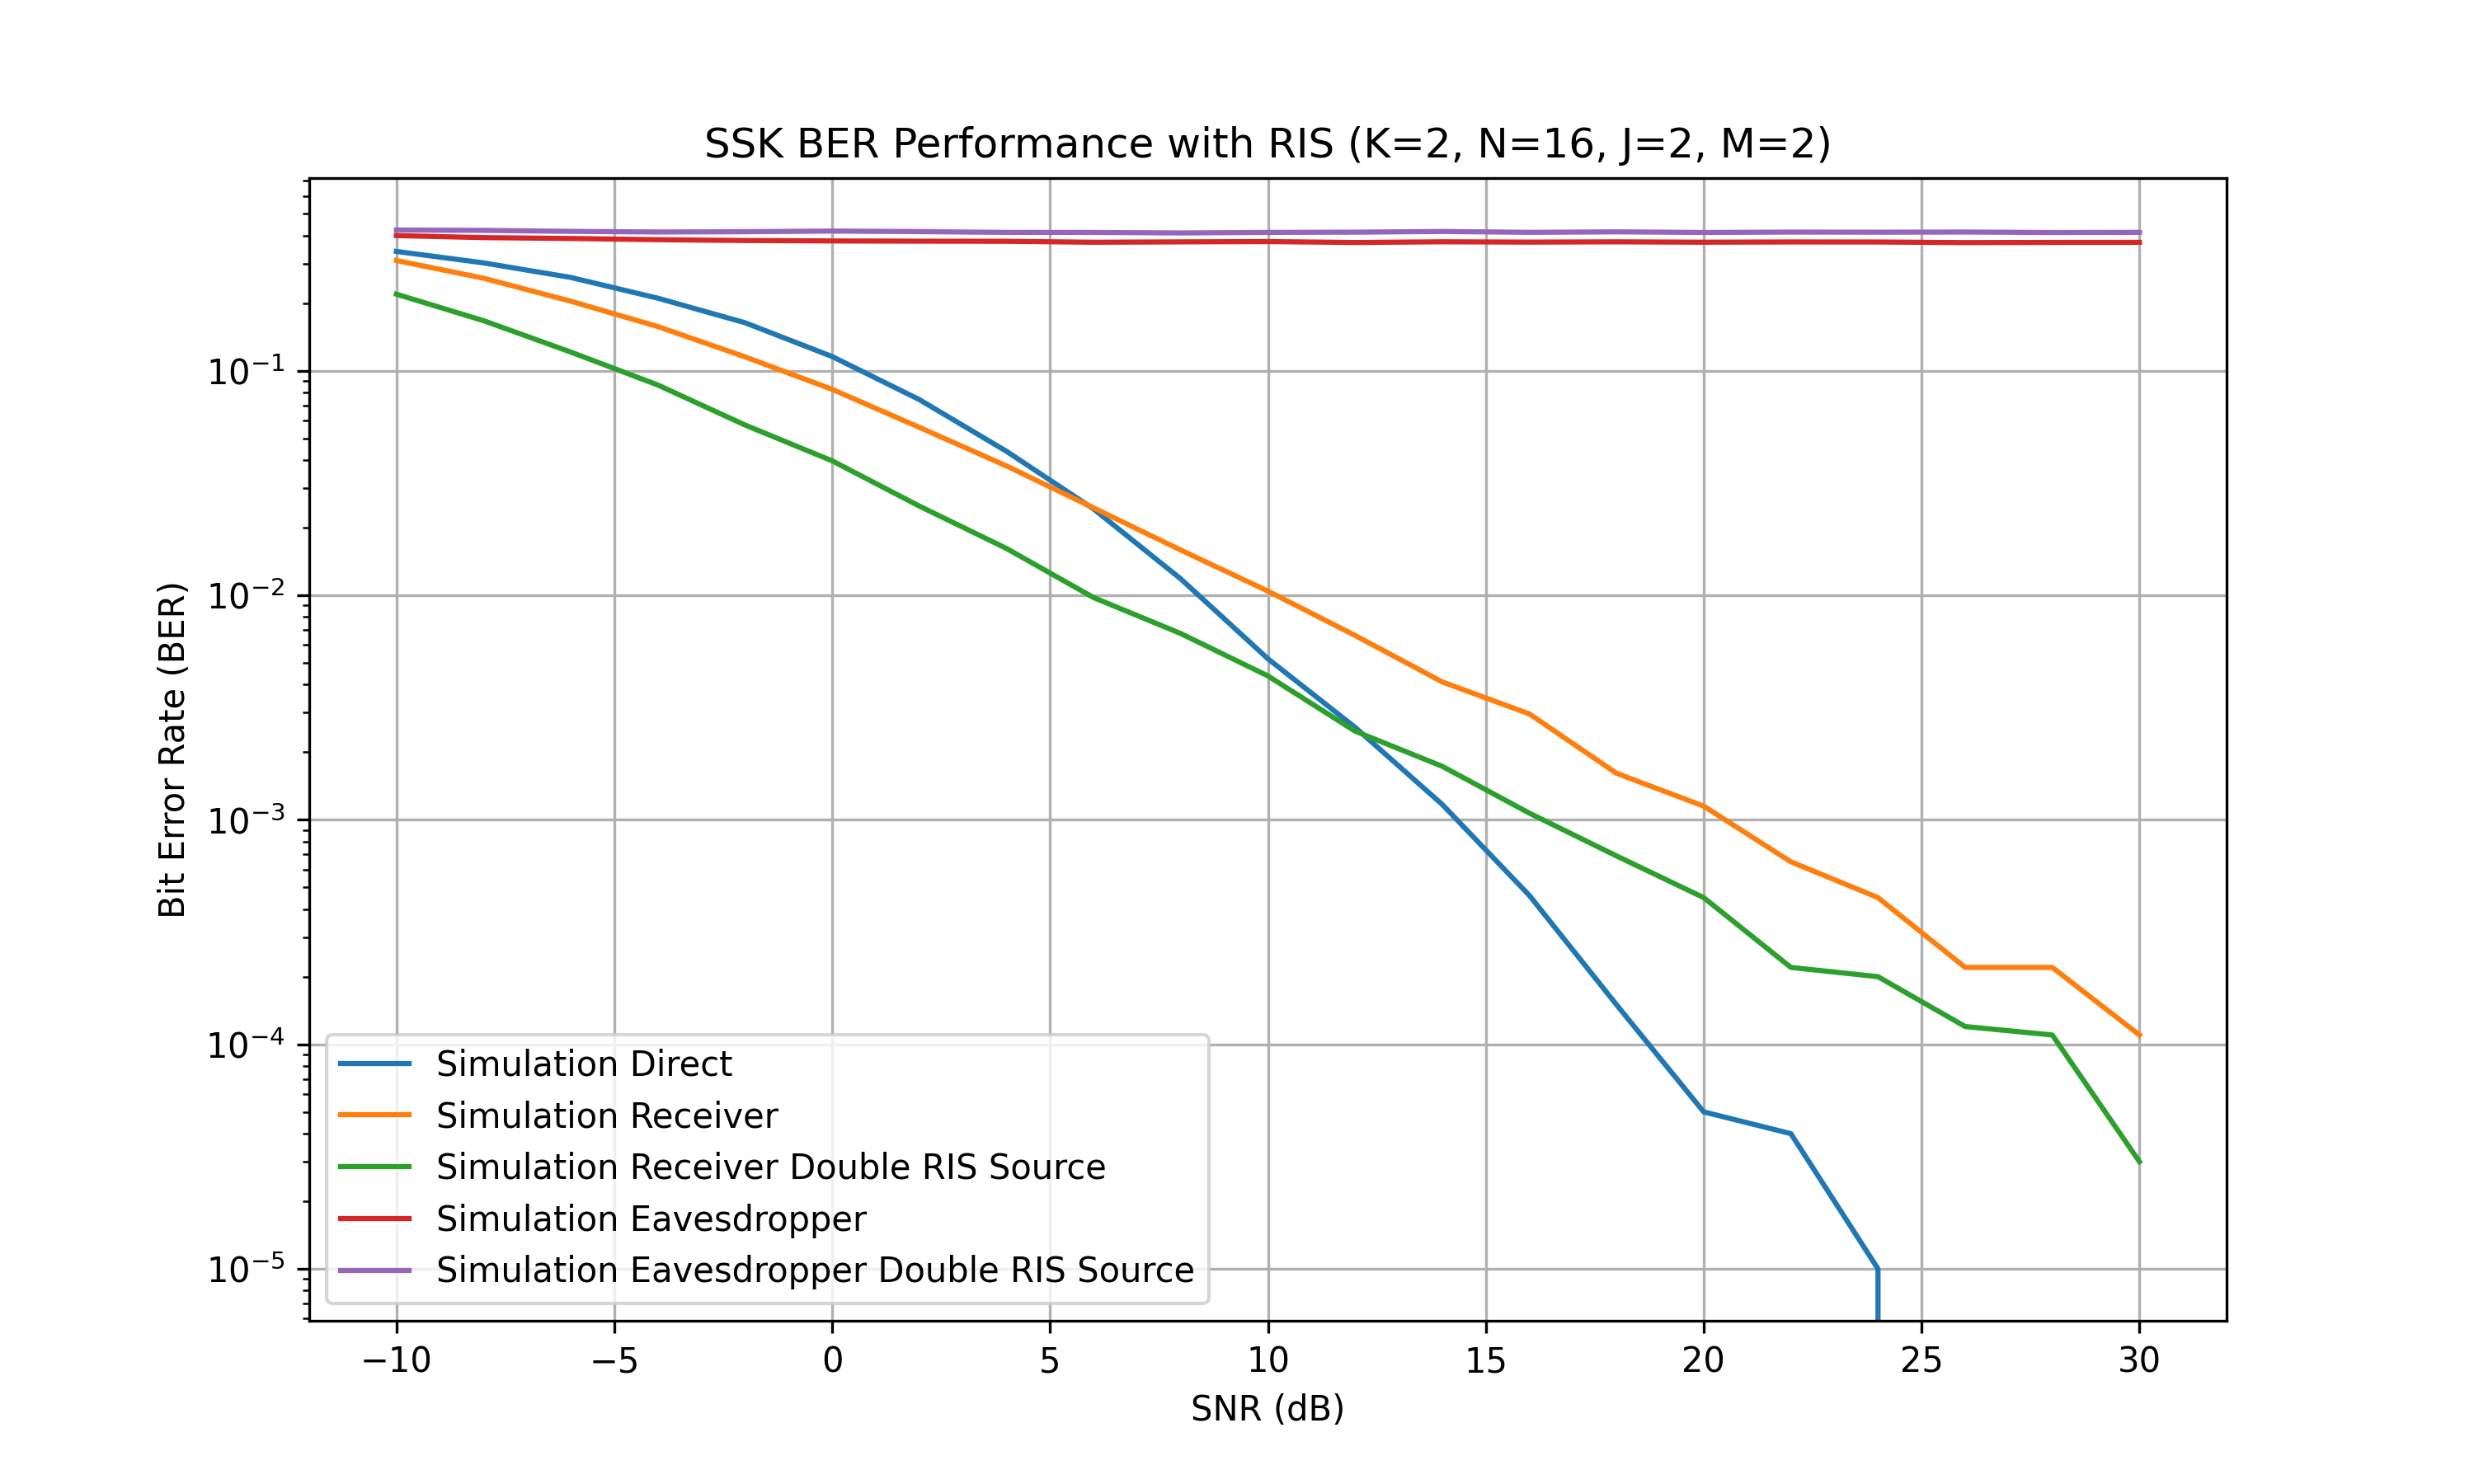
\includegraphics[width=0.9\linewidth]{imgs/ber-simulations/SSK BER Performance with RIS (K=2, N=16, J=2, M=2).png}
  \caption{SSK BER Performance with RIS (K=2, N=16, J=2, M=2)}
  \label{fig:simulation_j2_m2}
\end{figure}

Combining all together with two paths and double reflection to two receivers, our properties still hold strong.

\subsubsection{Theoretical conclusions}

From the graphs we can see that changes in the Signal to Noise Ratio (SNR) do not help the eavesdropper in understanding better the message. When there is a lot of noise, the performance is similar to the legitimate receivers, because no one is able to decipher the message.

When the noise level is much lower, and the signal strength much higher in comparison, the legitimate user understands the message much better, while the eavesdroppers do not. This is because even if the natural noise is reduced, the artificial noise caused by the unreadable RIS signal distorts the received communication for unwanted hearing users, and at the end the BER remains constant.

From \ref{fig:simulation_j1_m1}, we can already notice a lot of useful information. Firstly, the resulting graph comes out very similar to the one made by \cite{9328149}. This is good, because now we have confirmation of our base work, useful to also be confident about our extension and mathematical modifications. In their graph Fig 5.a, they show different lines based on multiple reflection coefficients $\eta$, while we used only $\eta = 0.9$, and different Rician Factors to model the power difference between the direct signal and the reflected one, while we used only the eavesdropper with value equal to $1$. Comparing those two particular lines to ours "Simulation Receiver" and "Simulation Eavesdropper".

We can focus better on our additions. Firstly, by adding the raw performance of the direct link, we can see that our reflected signal still gives for our legitimate users a solid link to communicate, that offers great performance even when considering the reflection coefficient loss $\eta$. Second, we can see that by adding a second reflection path with a double RIS source, our users get better signal while eavesdroppers get even more noise.

In the next graph \ref{fig:simulation_j2_m1} we can see how adding a second legitimate user does not influence the performance of our proposed general solution. This is great: our solution is more scalable, with the same capability to serve data securely. Adding more user constraints does not make our system more vulnerable or less understandable.

In \ref{fig:simulation_j1_m2} and \ref{fig:simulation_j2_m2} we can make similar considerations. Even by adding more reflections for each single path, our framework still shows high promises. We can see, however, that the legitimate receivers BER falls much faster. This is because without considering signal strength reductions due to path loss, multiplying the related matrices improves the overall signal calculated. This is why we also added a new type of simulation to our research, to test our framework with more realistic and specific scenarios.

\newpage
\subsection{BER realistic scenario simulation}

In this section, we evaluate our framework in more realistic spatial environments by creating BER heatmaps that show security performance across different physical locations. We model various path loss scenarios and analyze how they affect the security properties of our system.

We model the channel gain $H$ and the path loss based on the distance between the actors. We will define $\lambda$ as the wavelength of the signal, and $d$ as the distance between two actors.

\subsubsection{Channel gain calculation}

We model the Rician fading \cite{Rician_fading} matrix $\bm{\Xi}$, to consider possible fading due to multipath interference. Using the Shape Parameter $\tau$, defined as the ratio of the power contributions by line-of-sight path to the remaining multipaths, and the Scale parameter $\xi$, defined as the total power received in all paths, we can calculate

\begin{equation}
  \nu^2 = \frac{\tau \xi}{1 + \tau}
\end{equation}
\begin{equation}
  \sigma^2 = \frac{\xi}{2(1 + \tau)}
\end{equation}

and we can generate $\bm{\Xi}$ by creating a random complex matrix where the real and the imaginary values are extracted from a gaussian distribution $C(\frac{\nu}{\sqrt{2}}, \sigma)$ \cite{Rice_distribution}

Then, given an actor $r$ with $n_r$ antennas disposed as a \textit{uniform linear array}, we can define the \textit{unit spatial signature in the directional cosine $\Omega = cos \phi$} \cite{Fundamentals_Wireless_Communication_chapter7} as

\begin{equation}
  e_r(\Omega) = \frac{1}{\sqrt{n_r}}
  \begin{bmatrix}
    1                                \\
    exp(-j2\pi\Delta\Omega)          \\
    exp(-j2\pi2\Delta\Omega)         \\
    \vdots                           \\
    exp(-j2\pi(n_r - 1)\Delta\Omega) \\
  \end{bmatrix}
\end{equation}

where
\begin{itemize}
  \item $\Delta$ is the distance between the antennas (usually $\lambda / 2$)
  \item $\phi$ is the angle of incidence of the line-of-sight onto the actor antenna
\end{itemize}

and we can model the channel gain matrix \cite{Fundamentals_Wireless_Communication_chapter7} as

\begin{equation}
  \bm{H} = \bm{\Xi} \odot \sqrt{n_t n_r} exp(-j2 \pi d / \lambda) e_r(\Omega_r) e_t(\Omega_t)^H
\end{equation}

We will use this equation both for a direct transmission between two actors, or between an actor and a RIS.

\subsubsection{Path loss calculation}

We begin by modeling the free space path loss \cite{Free_space_path_loss} between two points as
\begin{equation}
  \bm{PL} = ((4 \pi / \lambda)^2 d^k)^{-\frac{1}{2}}
\end{equation}
where $k$ is equal to $2$ when the antennas are isotropic, meaning they radiate power uniformly in all directions in three dimensional space. We consider ideal conditions, and thus set $k = 2$.

For a direct LOS communication between the transmitter and another actor (either a legitimate receiver or an eavesdropper), the signal received from input $x$ would be

\begin{equation}
  y = \bm{PL}_B \cdot \bm{B}x
\end{equation}

Given a reflected signal with channel gain $GPH$, where
\begin{itemize}
  \item $\bm{G}$ is the communication transmitter-RIS
  \item $\bm{H}$ is the communication RIS-actors
  \item $\bm{P}$ is the RIS reflection coefficient diagonal matrix
\end{itemize}
we have two different LOS communications. We have different ways of calculating the total path loss:
\begin{itemize}
  \item we consider the RISs to be active, meaning they amplify the signal received before reflecting it and so they negate the path loss reduction. The signal received would be $y = PL_H \cdot GPHx$. As a result, in case of multiple RISs, only the last connection path loss is considered. We will call this as a \textit{active path loss}
  \item we consider two separate path losses, one for each LOS. The signal received would be $y = PL_G \cdot PL_H \cdot \bm{GPH}x$. In case of multiple RISs, we multiply the path loss of all connections. We will call this as a \textit{product path loss}. This usually represents a non directional, isotropic RIS, where the reflected signal is scattered uniformly across all directions and the path loss is significant.
  \item we consider one single path loss from the sum of the two distances ($d = d_{t-RIS} + d_{RIS-r}$). The signal received would be $y = PL_{G+H} \cdot \bm{GPH}x$. In case of multiple RISs, we add all the distances. We will call this as a \textit{sum path loss}. This is a simplification of a much more complex type of RIS, called directional RIS, which modulates the phase and magnitude of its elements to redirect the signal in a single direction. This regulation reduces the path loss caused by the second reflection, in relation to the number of elements $N$ of the RIS. It is possible to read more in the paper \cite{8888223}. It is important to note that, while we are showing results of how a scenario with this type of path loss may act, we will just vary the calculation of the path loss for each point in the map, and will not make any calculations of directional phases themselves. The RIS would still look like an uniform sending relay, and it is included in the document to show the potentiality of our framework in that condition. So for the \textit{sum path loss}, it is important to remember this theoretical limitation. For example, we will show the BER for two different receivers in different locations and various situations, but of course it not be possible to serve in multiple direction for that type of RIS. Mathematically, you could see our graphs of this kind as showing the situation where we have  $\lim_{X \to \infty} X$ RIS, all in the same position, each one directed to a different point of the map, with none interfering with each other. It is most certainly an interesting topic for a later research, the actual implementation of our framework with the constraint of directionality of the RIS. This could be done by putting more constraints on the vector $q$ in \eqref{q_random_vector}.
\end{itemize}

We will show the main graph, showing the heatmap of the BER for each square, and two or three graphs, showing the logarithmic heatmap of the power received in that point from the transmitter of from a reflection passing through a RIS. For the BER, you could consider all spots not signed by a label as a possible eavesdropper location. \textbf{T} represents the transmitter, $\bm{P}_m$ are the RIS and $\bm{R}_j$ the legitimate receivers.

\subsubsection{Single angle of reflection, aided by 1 RIS}

Here we have a standard scenario where the transmitter has only a conical view between two buildings, and the receivers do not have direct LOS. What we want to show is that without LOS the message is completely unreadable except for the legitimate users, while the spots in LOS with the transmitter still receive various levels of noise.

For all of the three kinds of path loss, we will have the following parameters: $\lambda = 0.08m$, as standard for 5G connections, $ \tau = 0.6, \xi = 1, \eta = 0.9, SNR = 10dB, K = 4, N = 25$. In particular, we want to use for this scenario a higher number of antennas per actor and reflecting elements per RIS to show: 1) a bit more complex configuration that the standard $K = 2, N = 16$; 2) show that the BER does have an upper limit on 0.5, the value of random guessing. This is because, even if a higher $K$ could make one suppose you have only $1/K$ probability of guessing the turned on antenna, the actual bit representation is only made of $0$ and $1$, and thus the probability of error for each bit is $0.5$.

\begin{figure}[H]
  \centering
  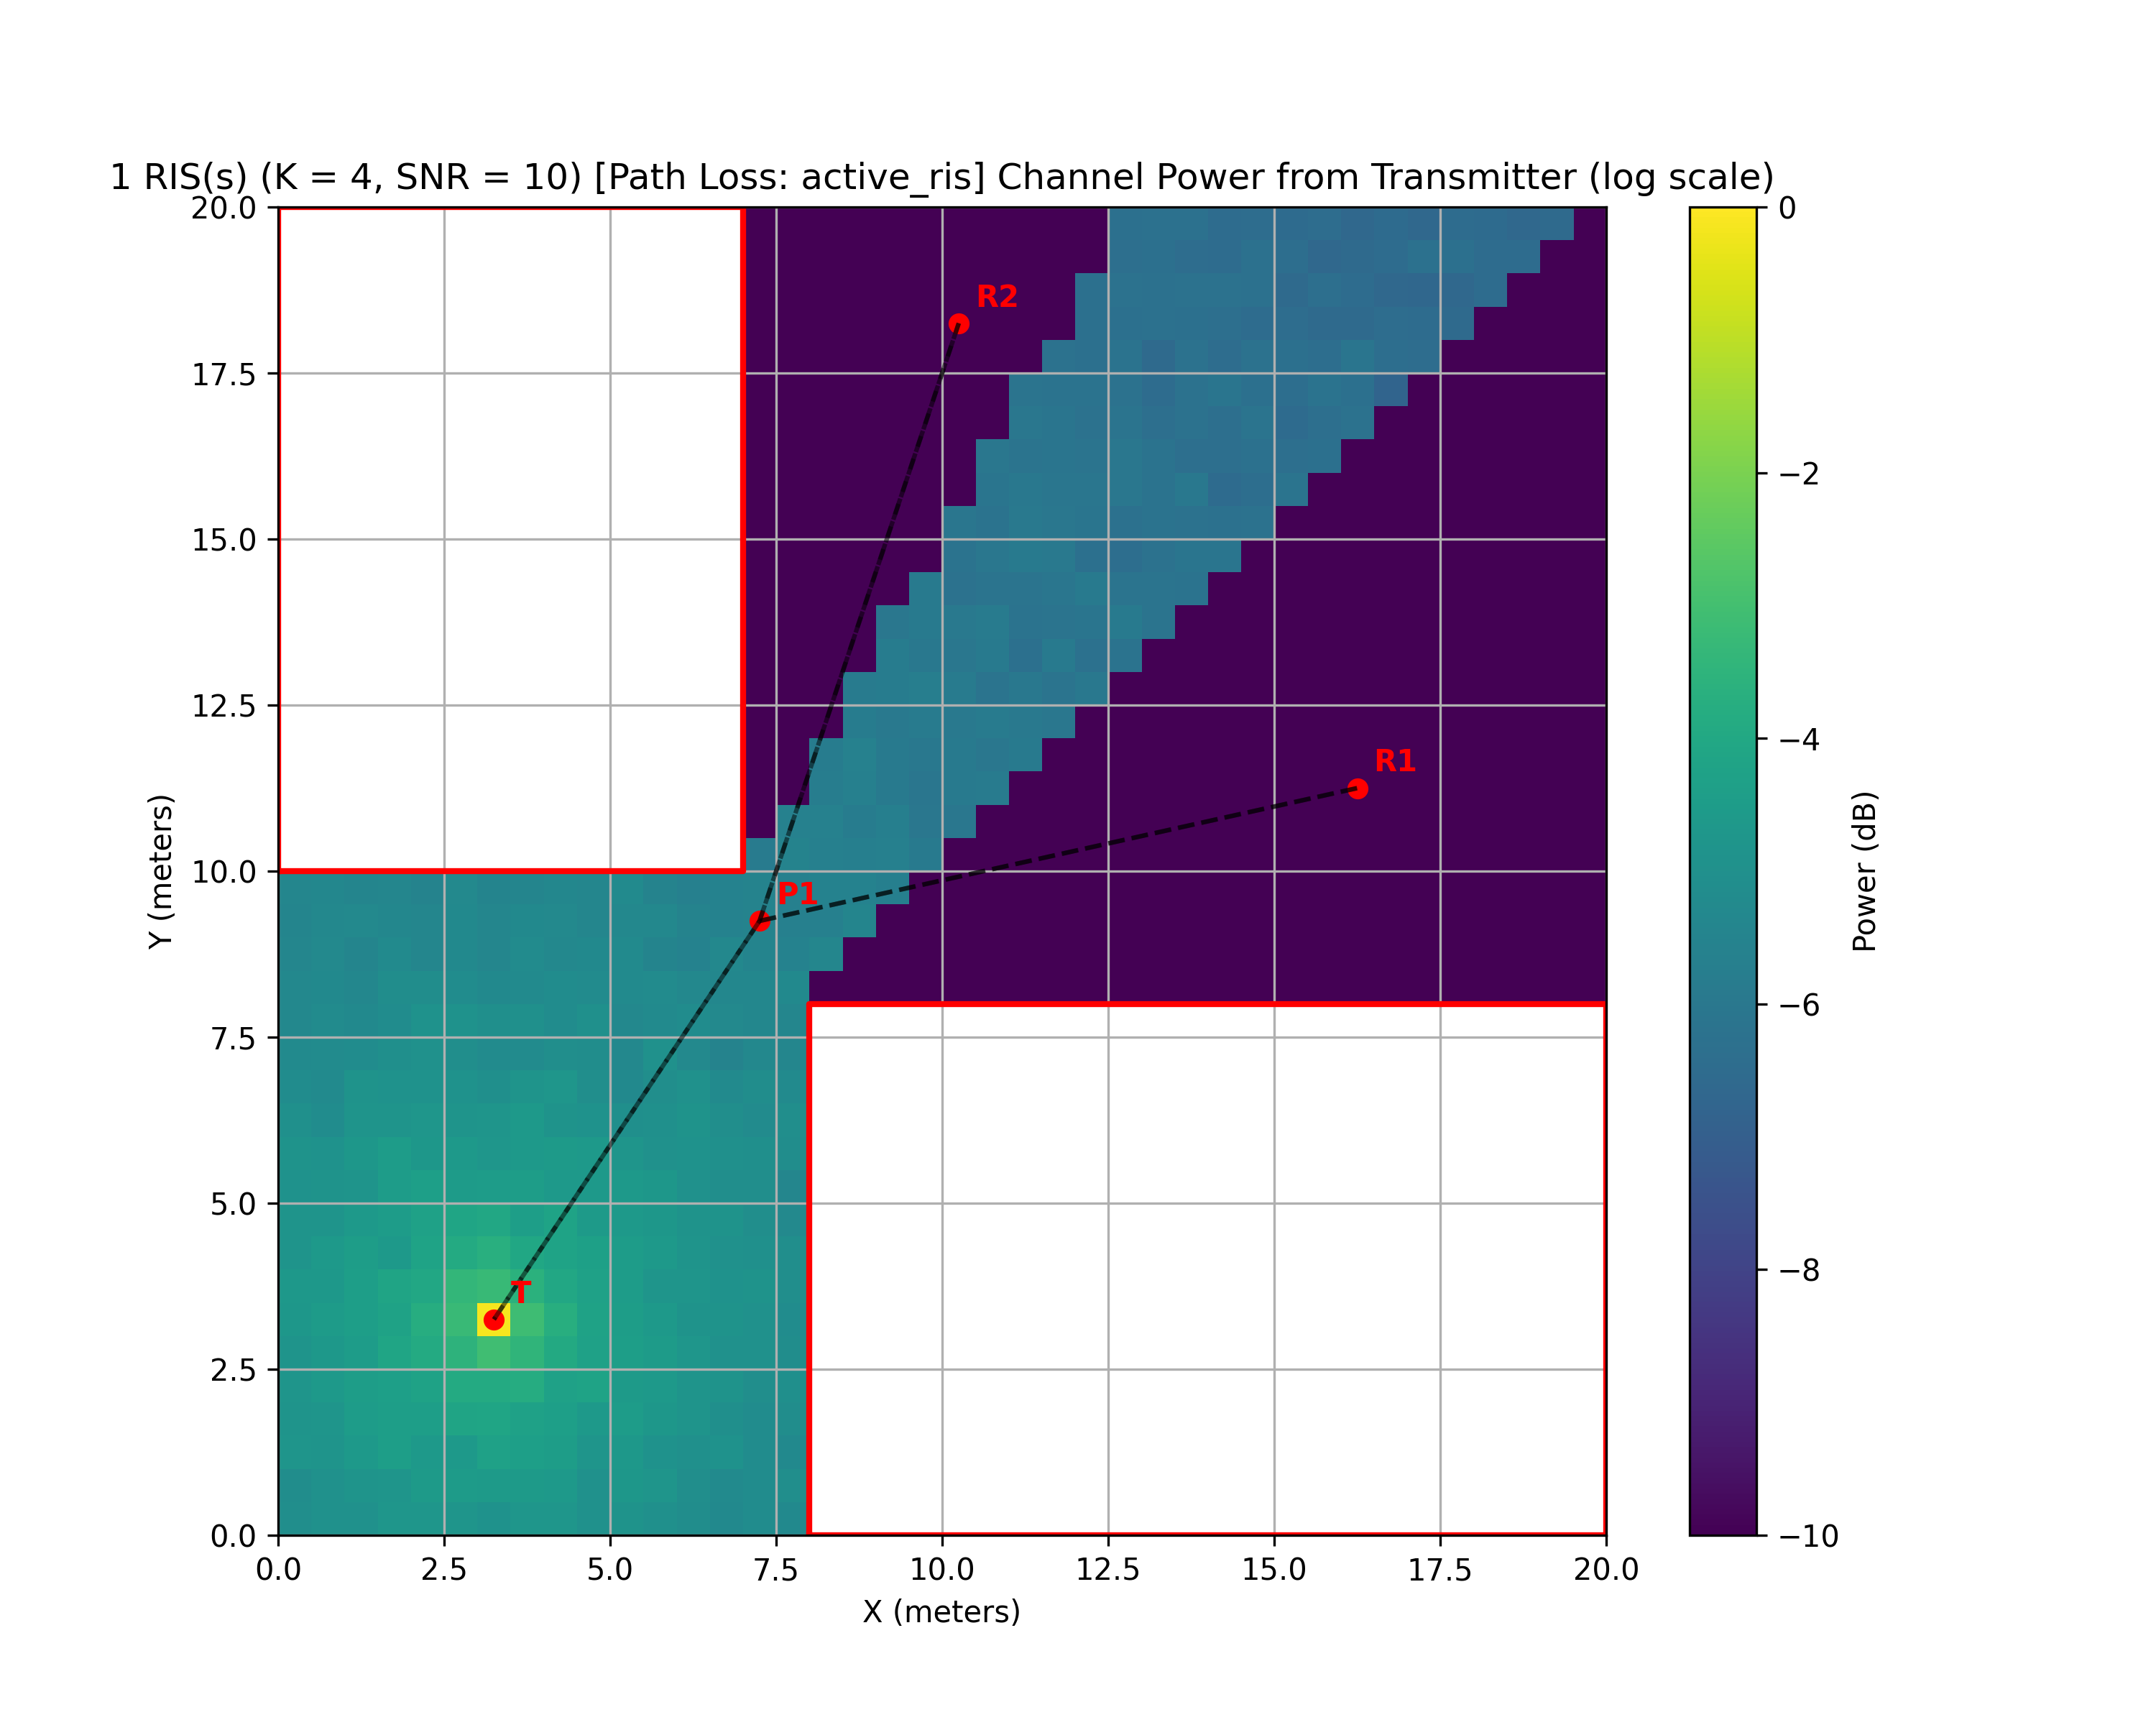
\includegraphics[width=0.7\linewidth]{imgs/heatmap-simulations/1 RIS(s) (K = 4, SNR = 10) [Path Loss_ active_ris] Channel Power from Transmitter (log scale).png}
  \caption{1 RIS(s) Channel Power from Transmitter (log scale)}
\end{figure}

\paragraph*{Path loss: active}

We can see here how this type of path loss ensures that in the vicinity of the RIS the Bit Error Rate remains very high, thanks to the active power component of the RIS itself.

We can see the reflected signal from the RIS has the RIS itself as the center.

\begin{figure}[H]
  \centering
  \begin{subfigure}[b]{0.48\textwidth}
    \centering
    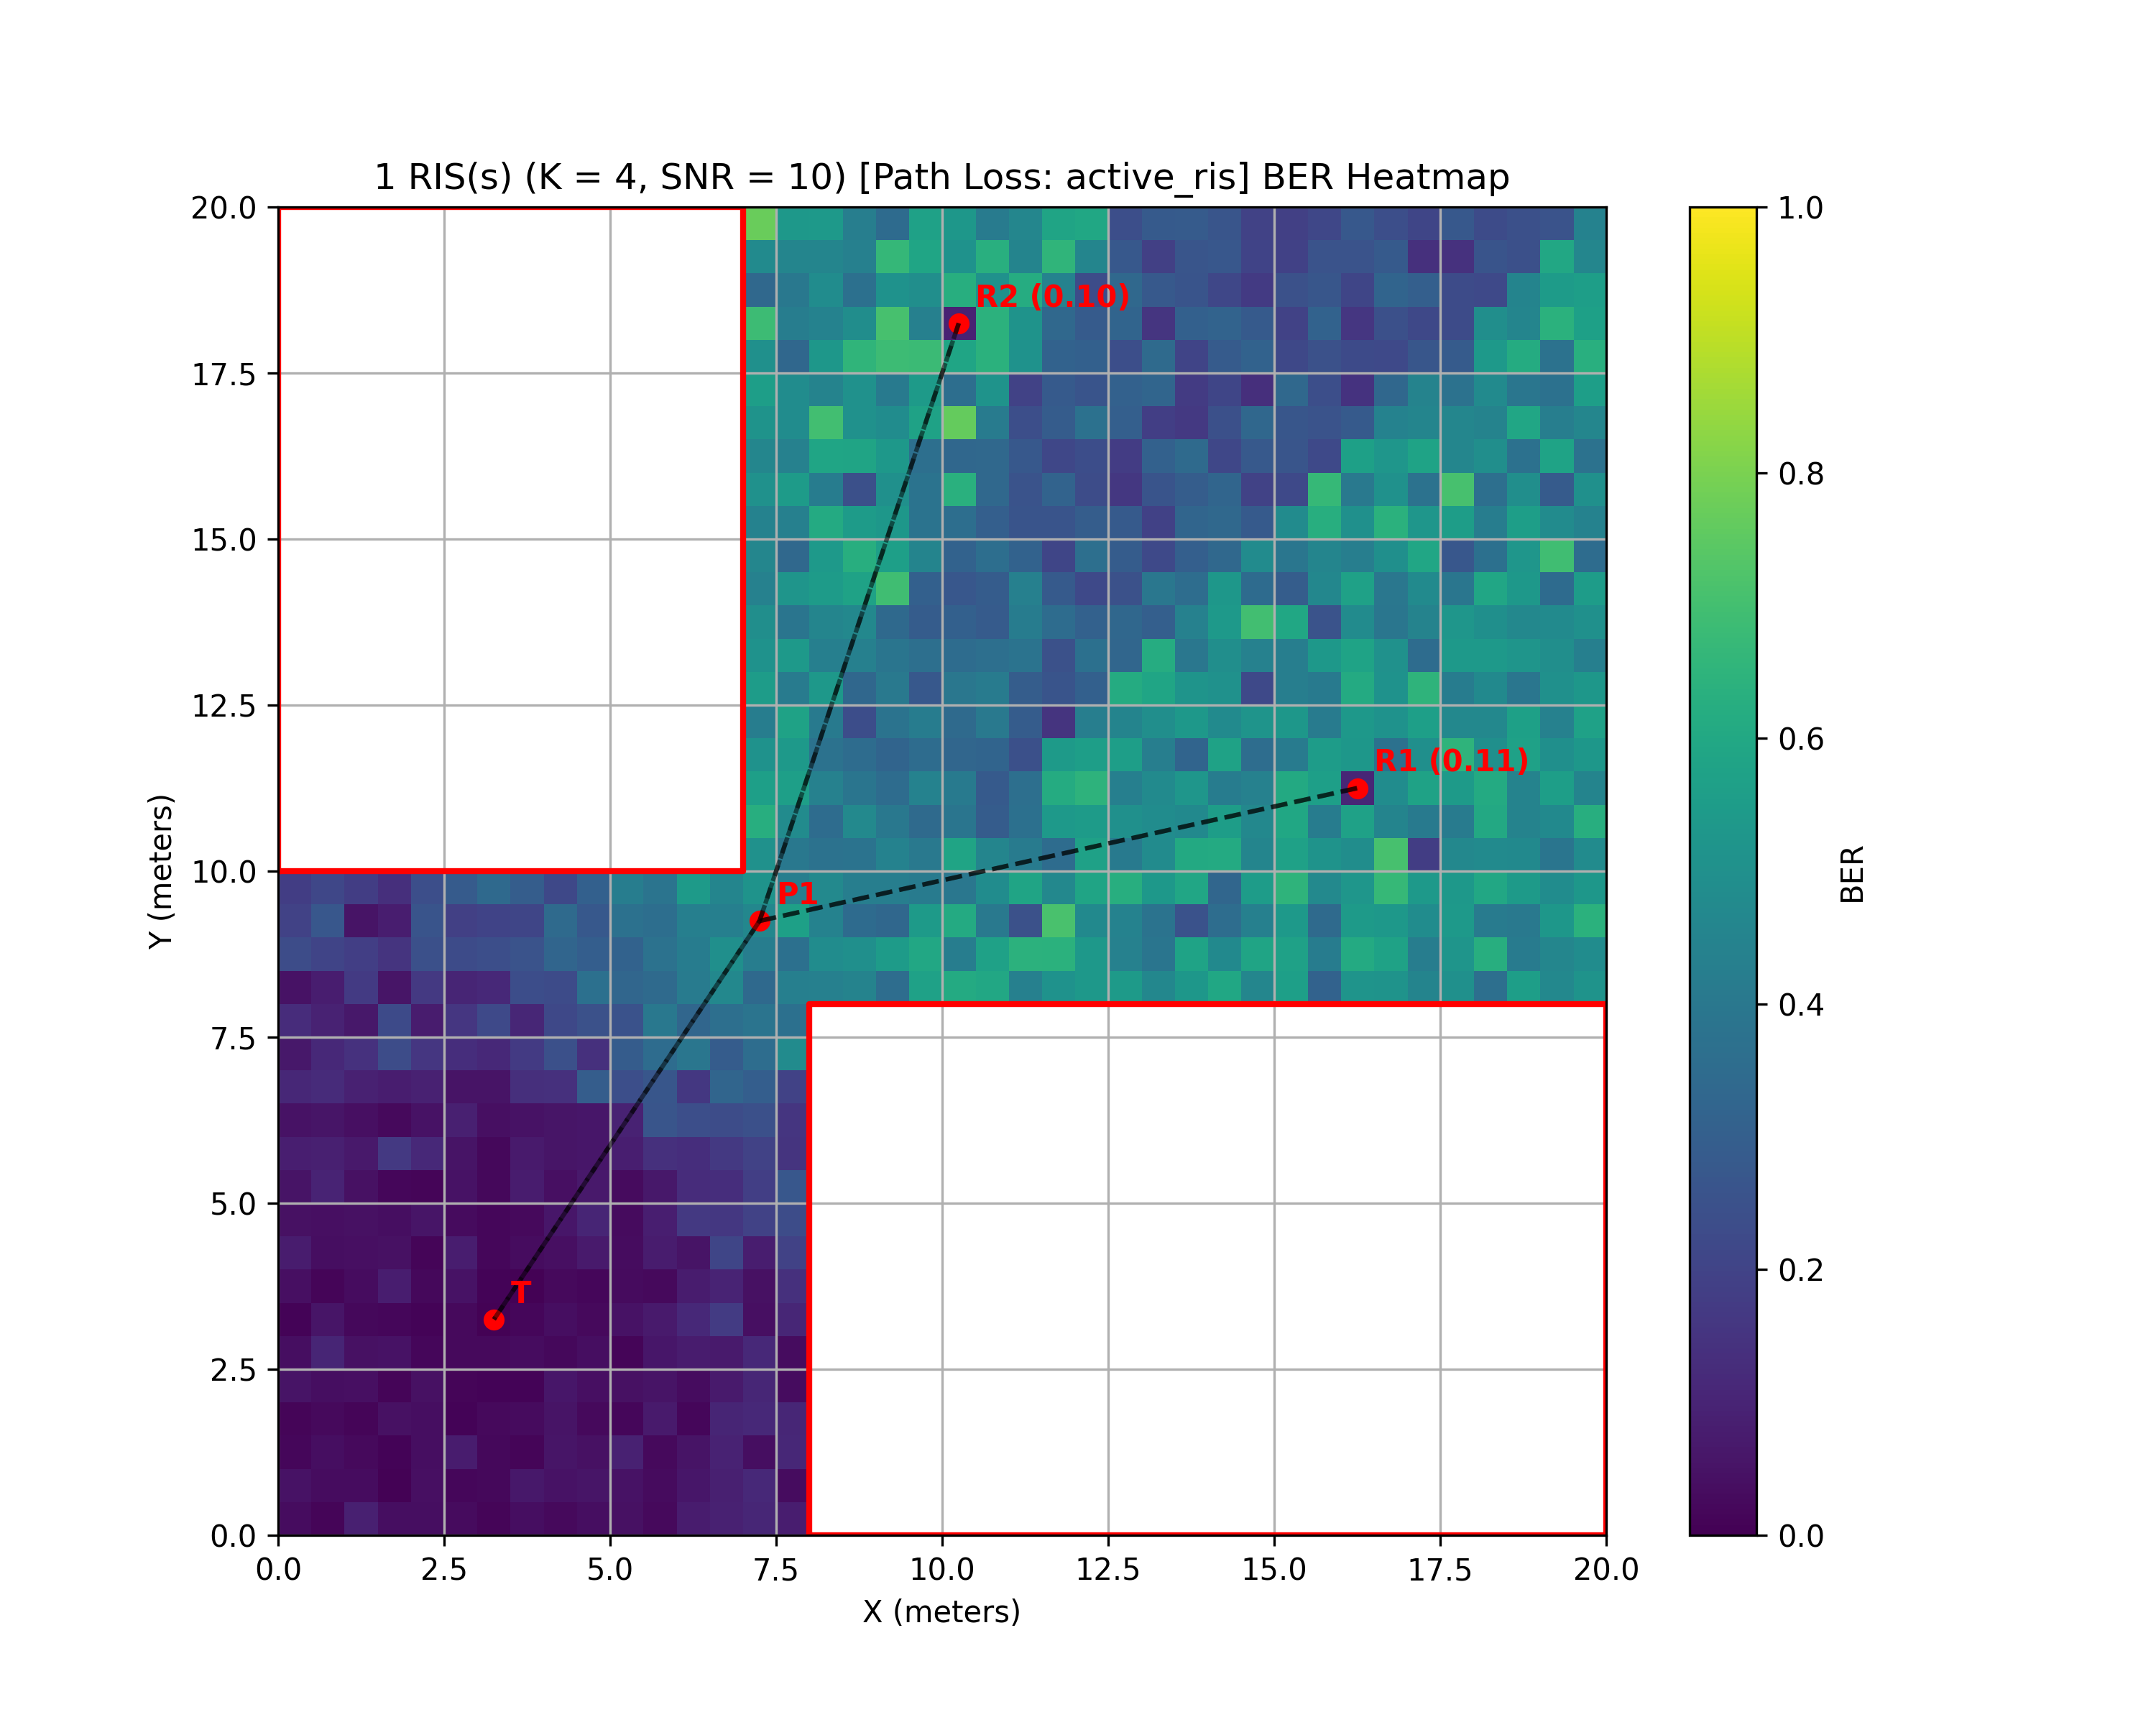
\includegraphics[width=\textwidth]{imgs/heatmap-simulations/1 RIS(s) (K = 4, SNR = 10) [Path Loss_ active_ris] BER Heatmap.png}
    \caption{BER Heatmap}
  \end{subfigure}
  \hfill
  \begin{subfigure}[b]{0.48\textwidth}
    \centering
    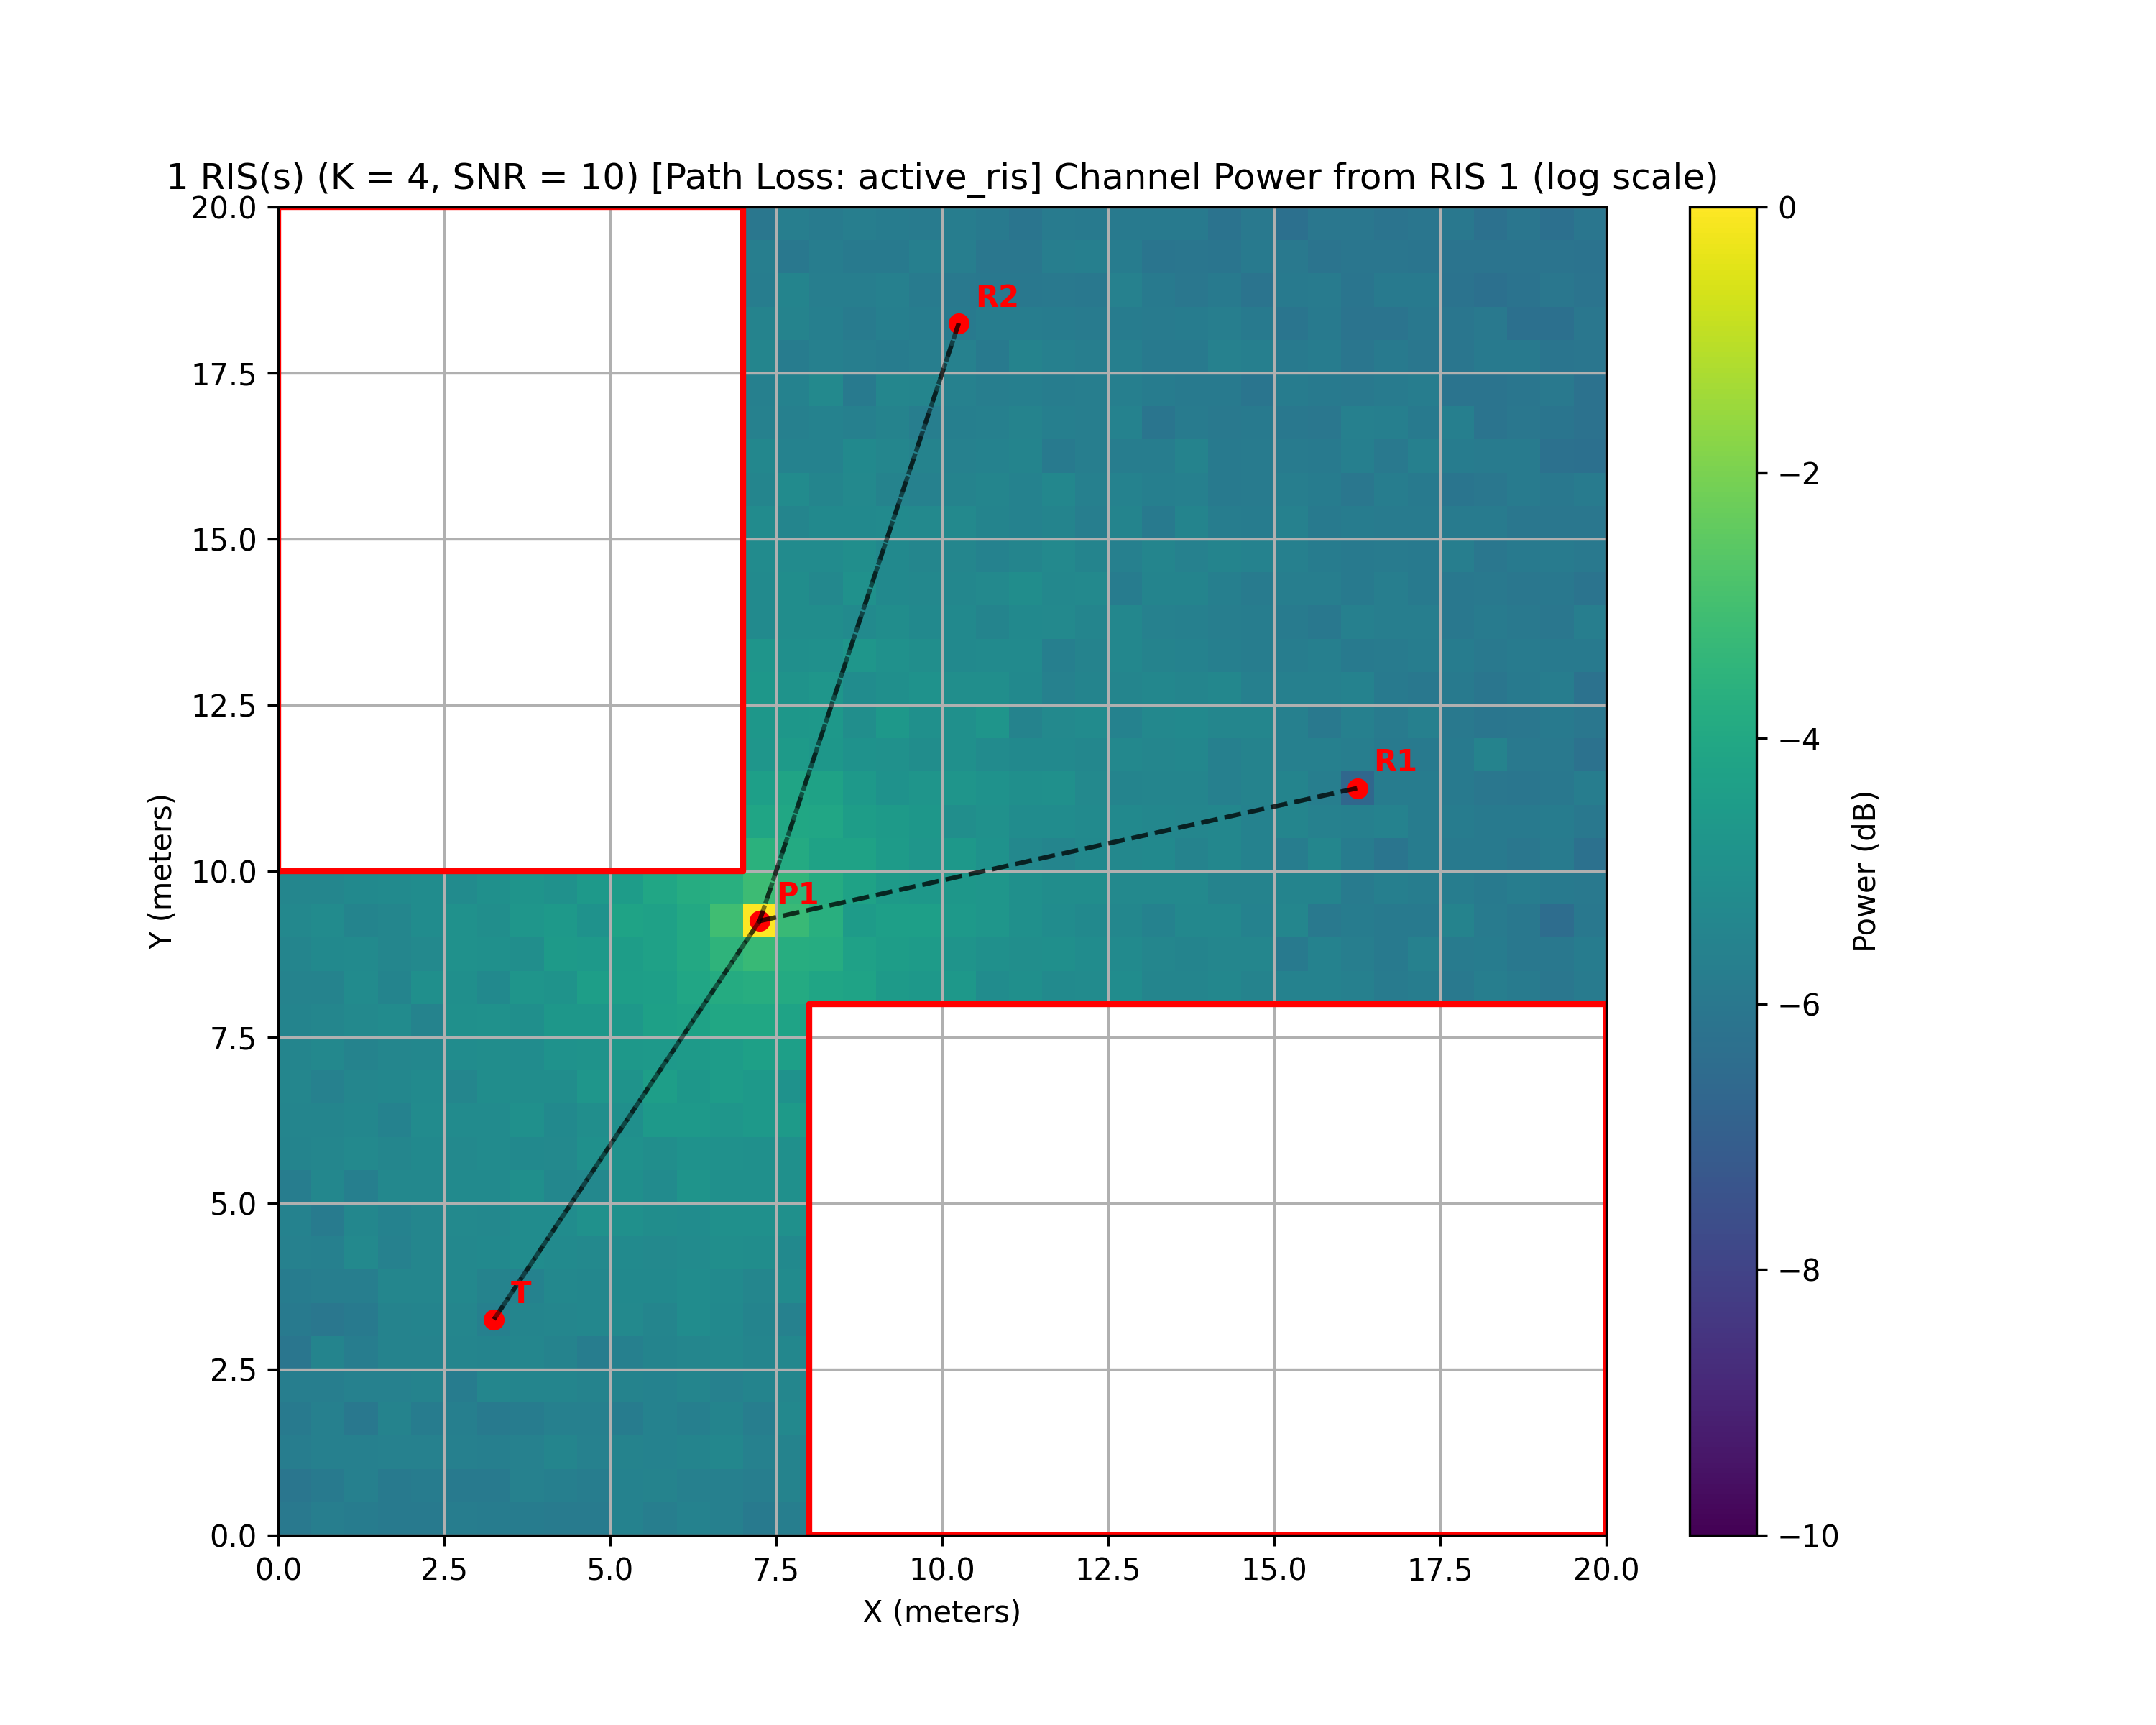
\includegraphics[width=\textwidth]{imgs/heatmap-simulations/1 RIS(s) (K = 4, SNR = 10) [Path Loss_ active_ris] Channel Power from RIS 1 (log scale).png}
    \caption{Channel Power from RIS 1 (log scale)}
  \end{subfigure}
  \caption{1 RIS(s) [Path Loss: active ris]}
\end{figure}

\paragraph*{Path loss: product}

With this type of path loss, the signal coming from the RIS has significantly less power than the direct link from the transmitter, and cannot influence significantly the outcome. Outside LOS, the framework still works as expected.

The power of the signal reflected from the RIS is so low, it does not show in the heatmap, as it is lower than $1e-10$.

\begin{figure}[H]
  \centering
  \begin{subfigure}[b]{0.48\textwidth}
    \centering
    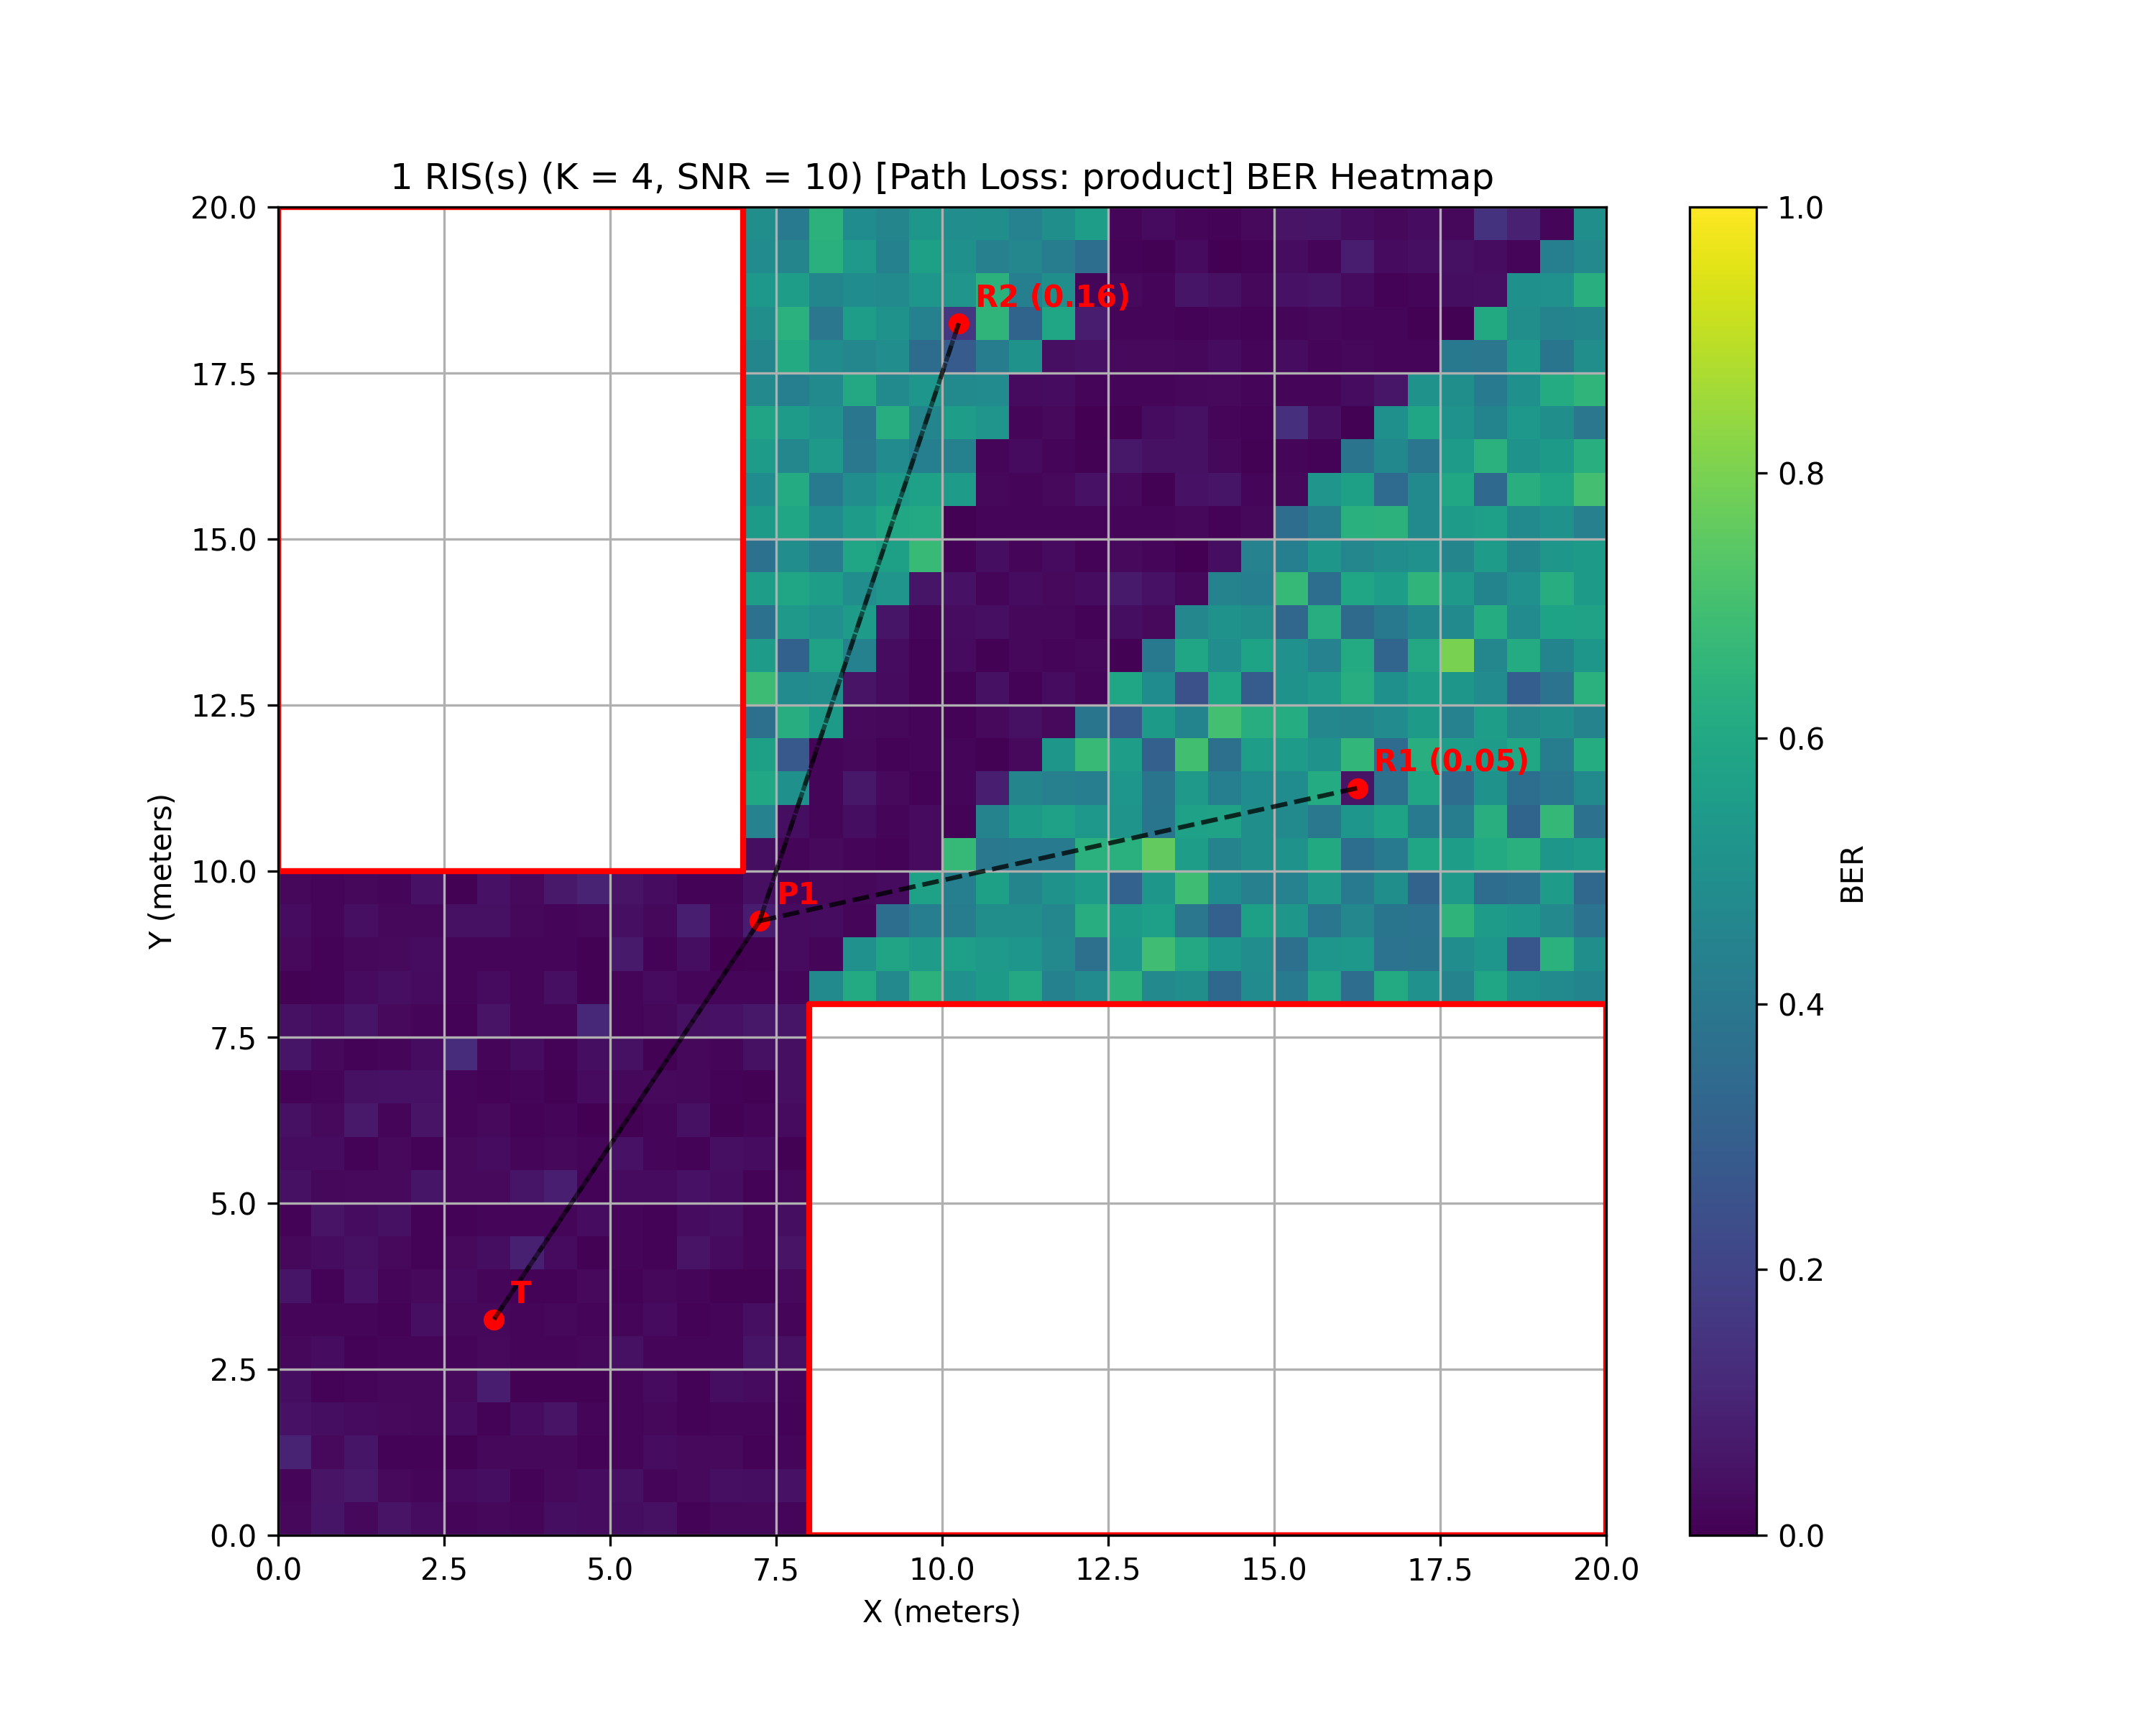
\includegraphics[width=\textwidth]{imgs/heatmap-simulations/1 RIS(s) (K = 4, SNR = 10) [Path Loss_ product] BER Heatmap.png}
    \caption{BER Heatmap}
  \end{subfigure}
  \hfill
  \begin{subfigure}[b]{0.48\textwidth}
    \centering
    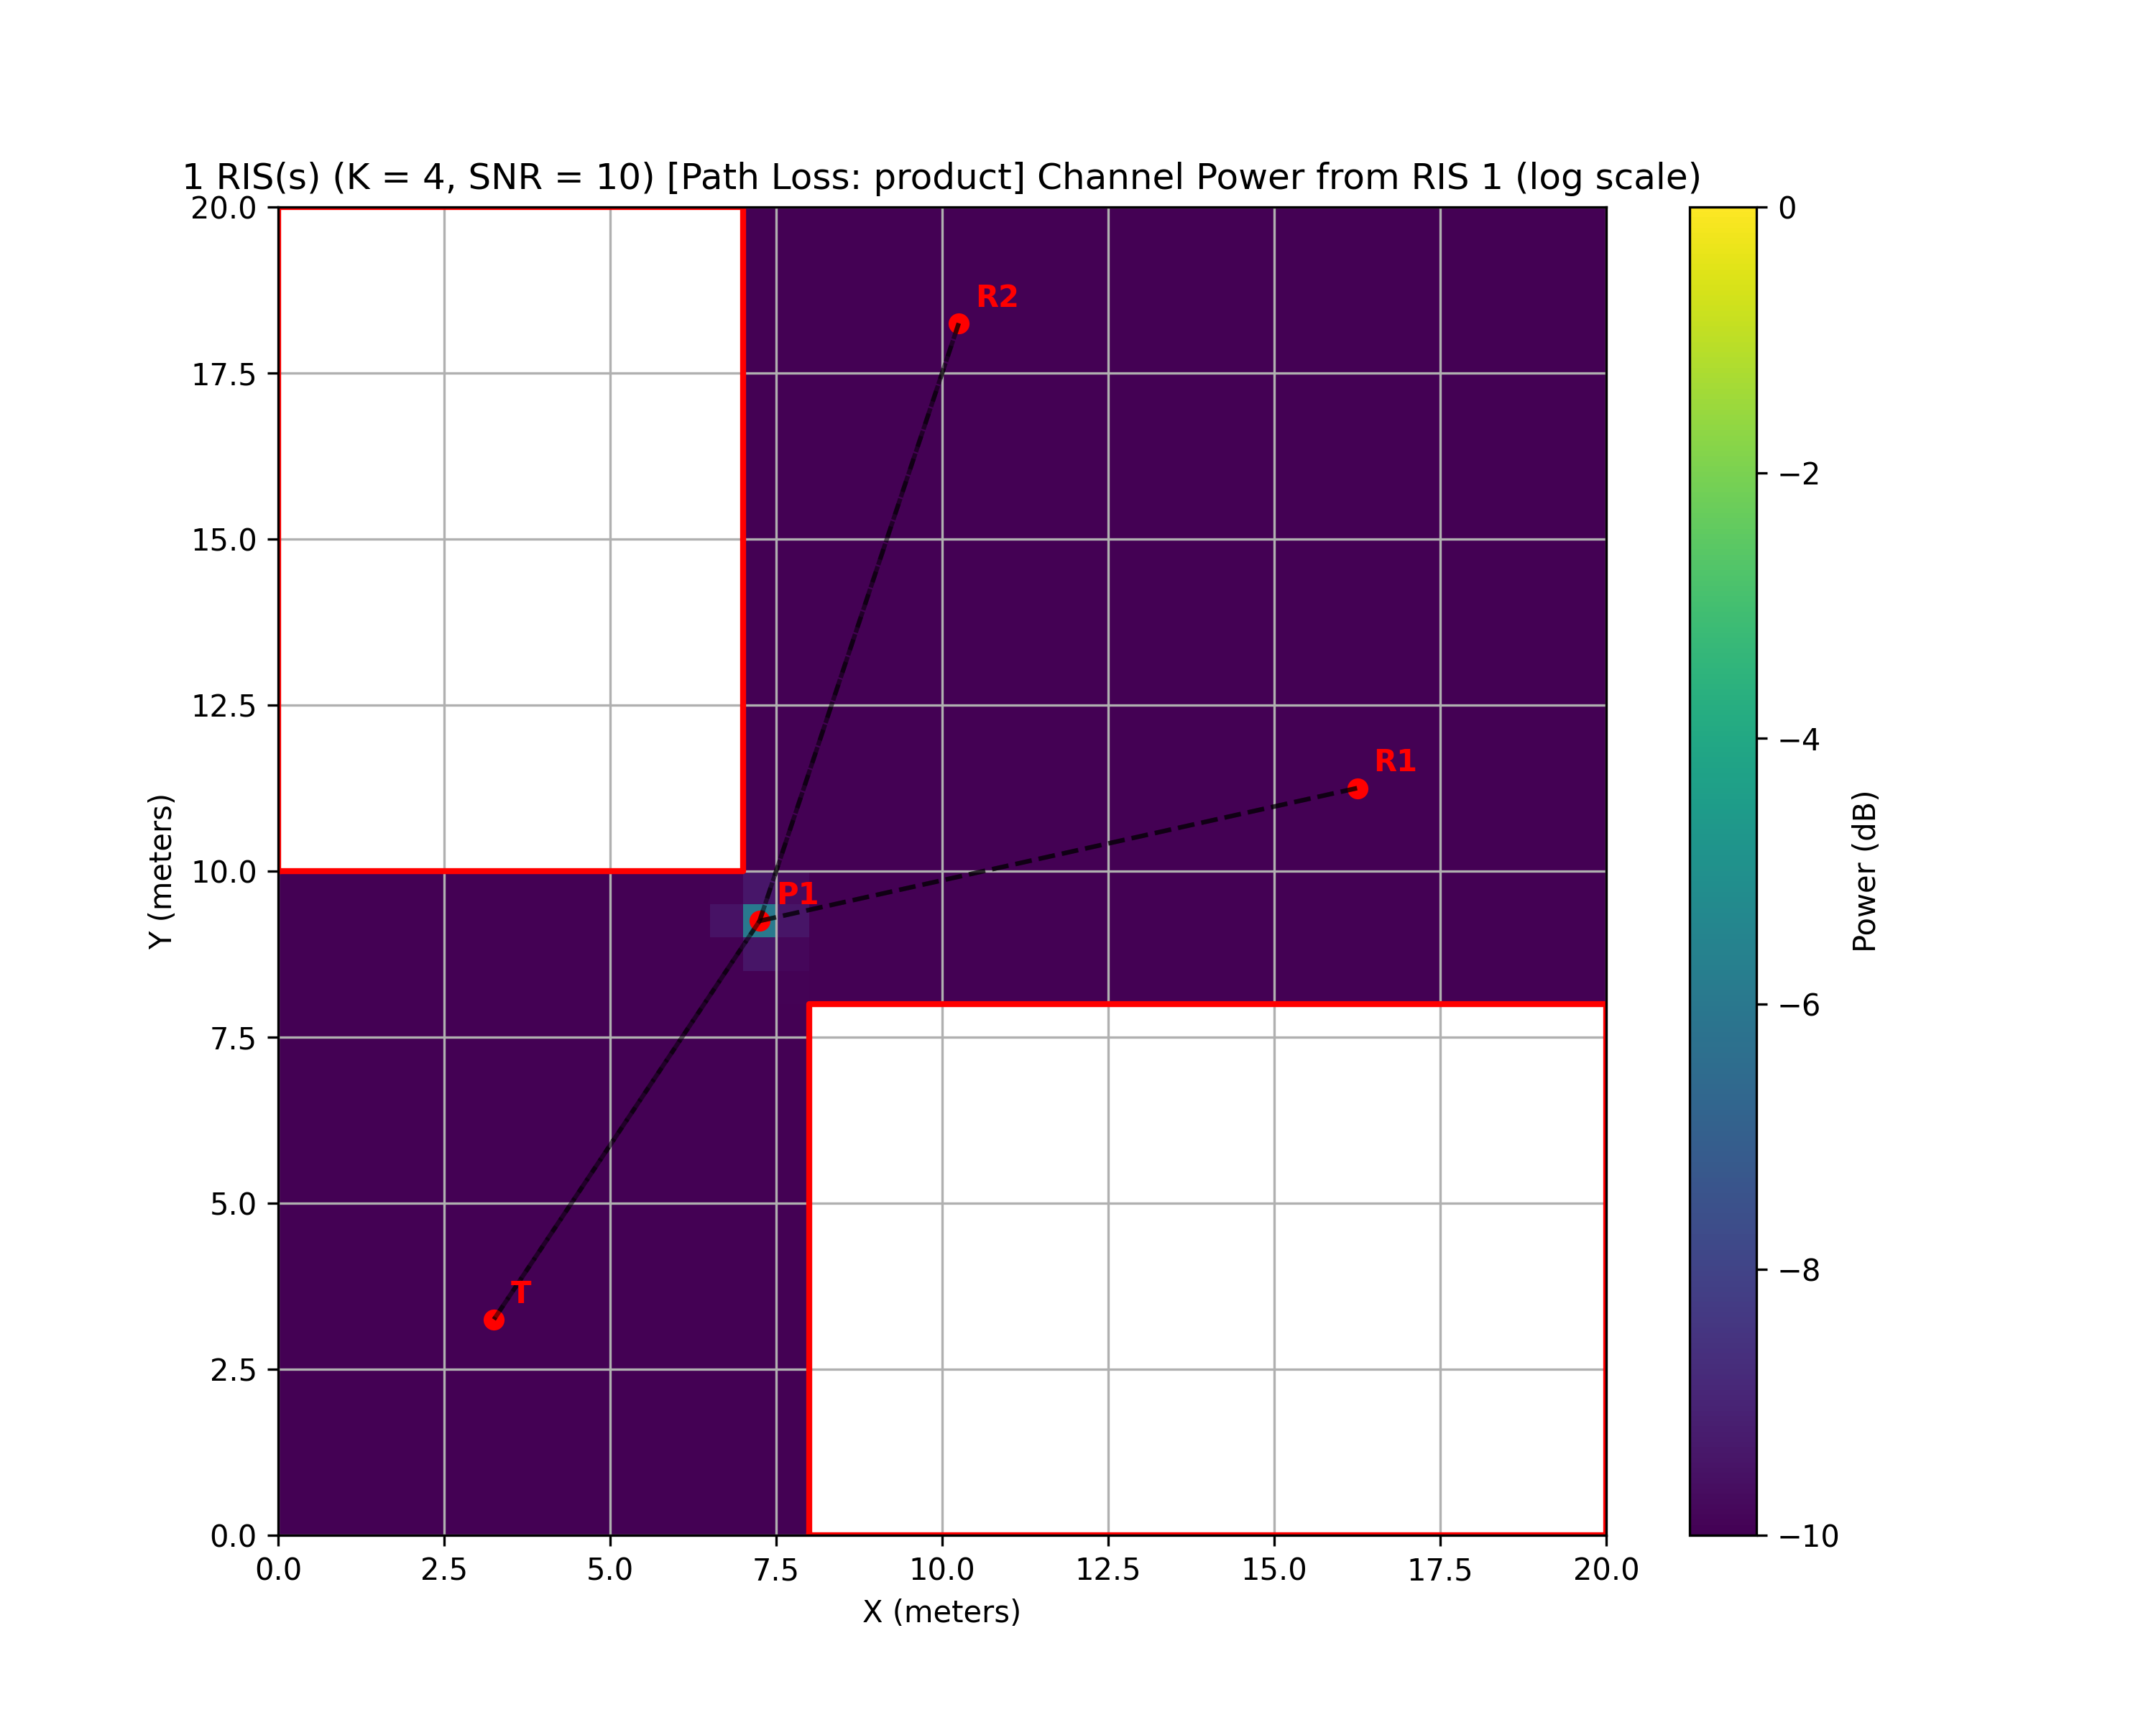
\includegraphics[width=\textwidth]{imgs/heatmap-simulations/1 RIS(s) (K = 4, SNR = 10) [Path Loss_ product] Channel Power from RIS 1 (log scale).png}
    \caption{Channel Power from RIS 1 (log scale)}
  \end{subfigure}
  \caption{1 RIS(s) [Path Loss: product]}
\end{figure}

\paragraph*{Path loss: sum}
This is the path loss that better confirms our previous BER analysis. Without LOS, the BER for eavesdropper is stable at 0.5, the same as random guessing. With LOS, the RIS is still able to influence significantly the outcome, with more noise that reduces the BER at 0.3

We can see how the power coming from the RIS reflection looks more uniform than the others. This is because, as we said before, this type of path loss actually models a directional RIS. The total result of this graph does not exist. You could see them as the union of all the possible graphs considering a single direction of the reflection.

\begin{figure}[H]
  \centering
  \begin{subfigure}[b]{0.48\textwidth}
    \centering
    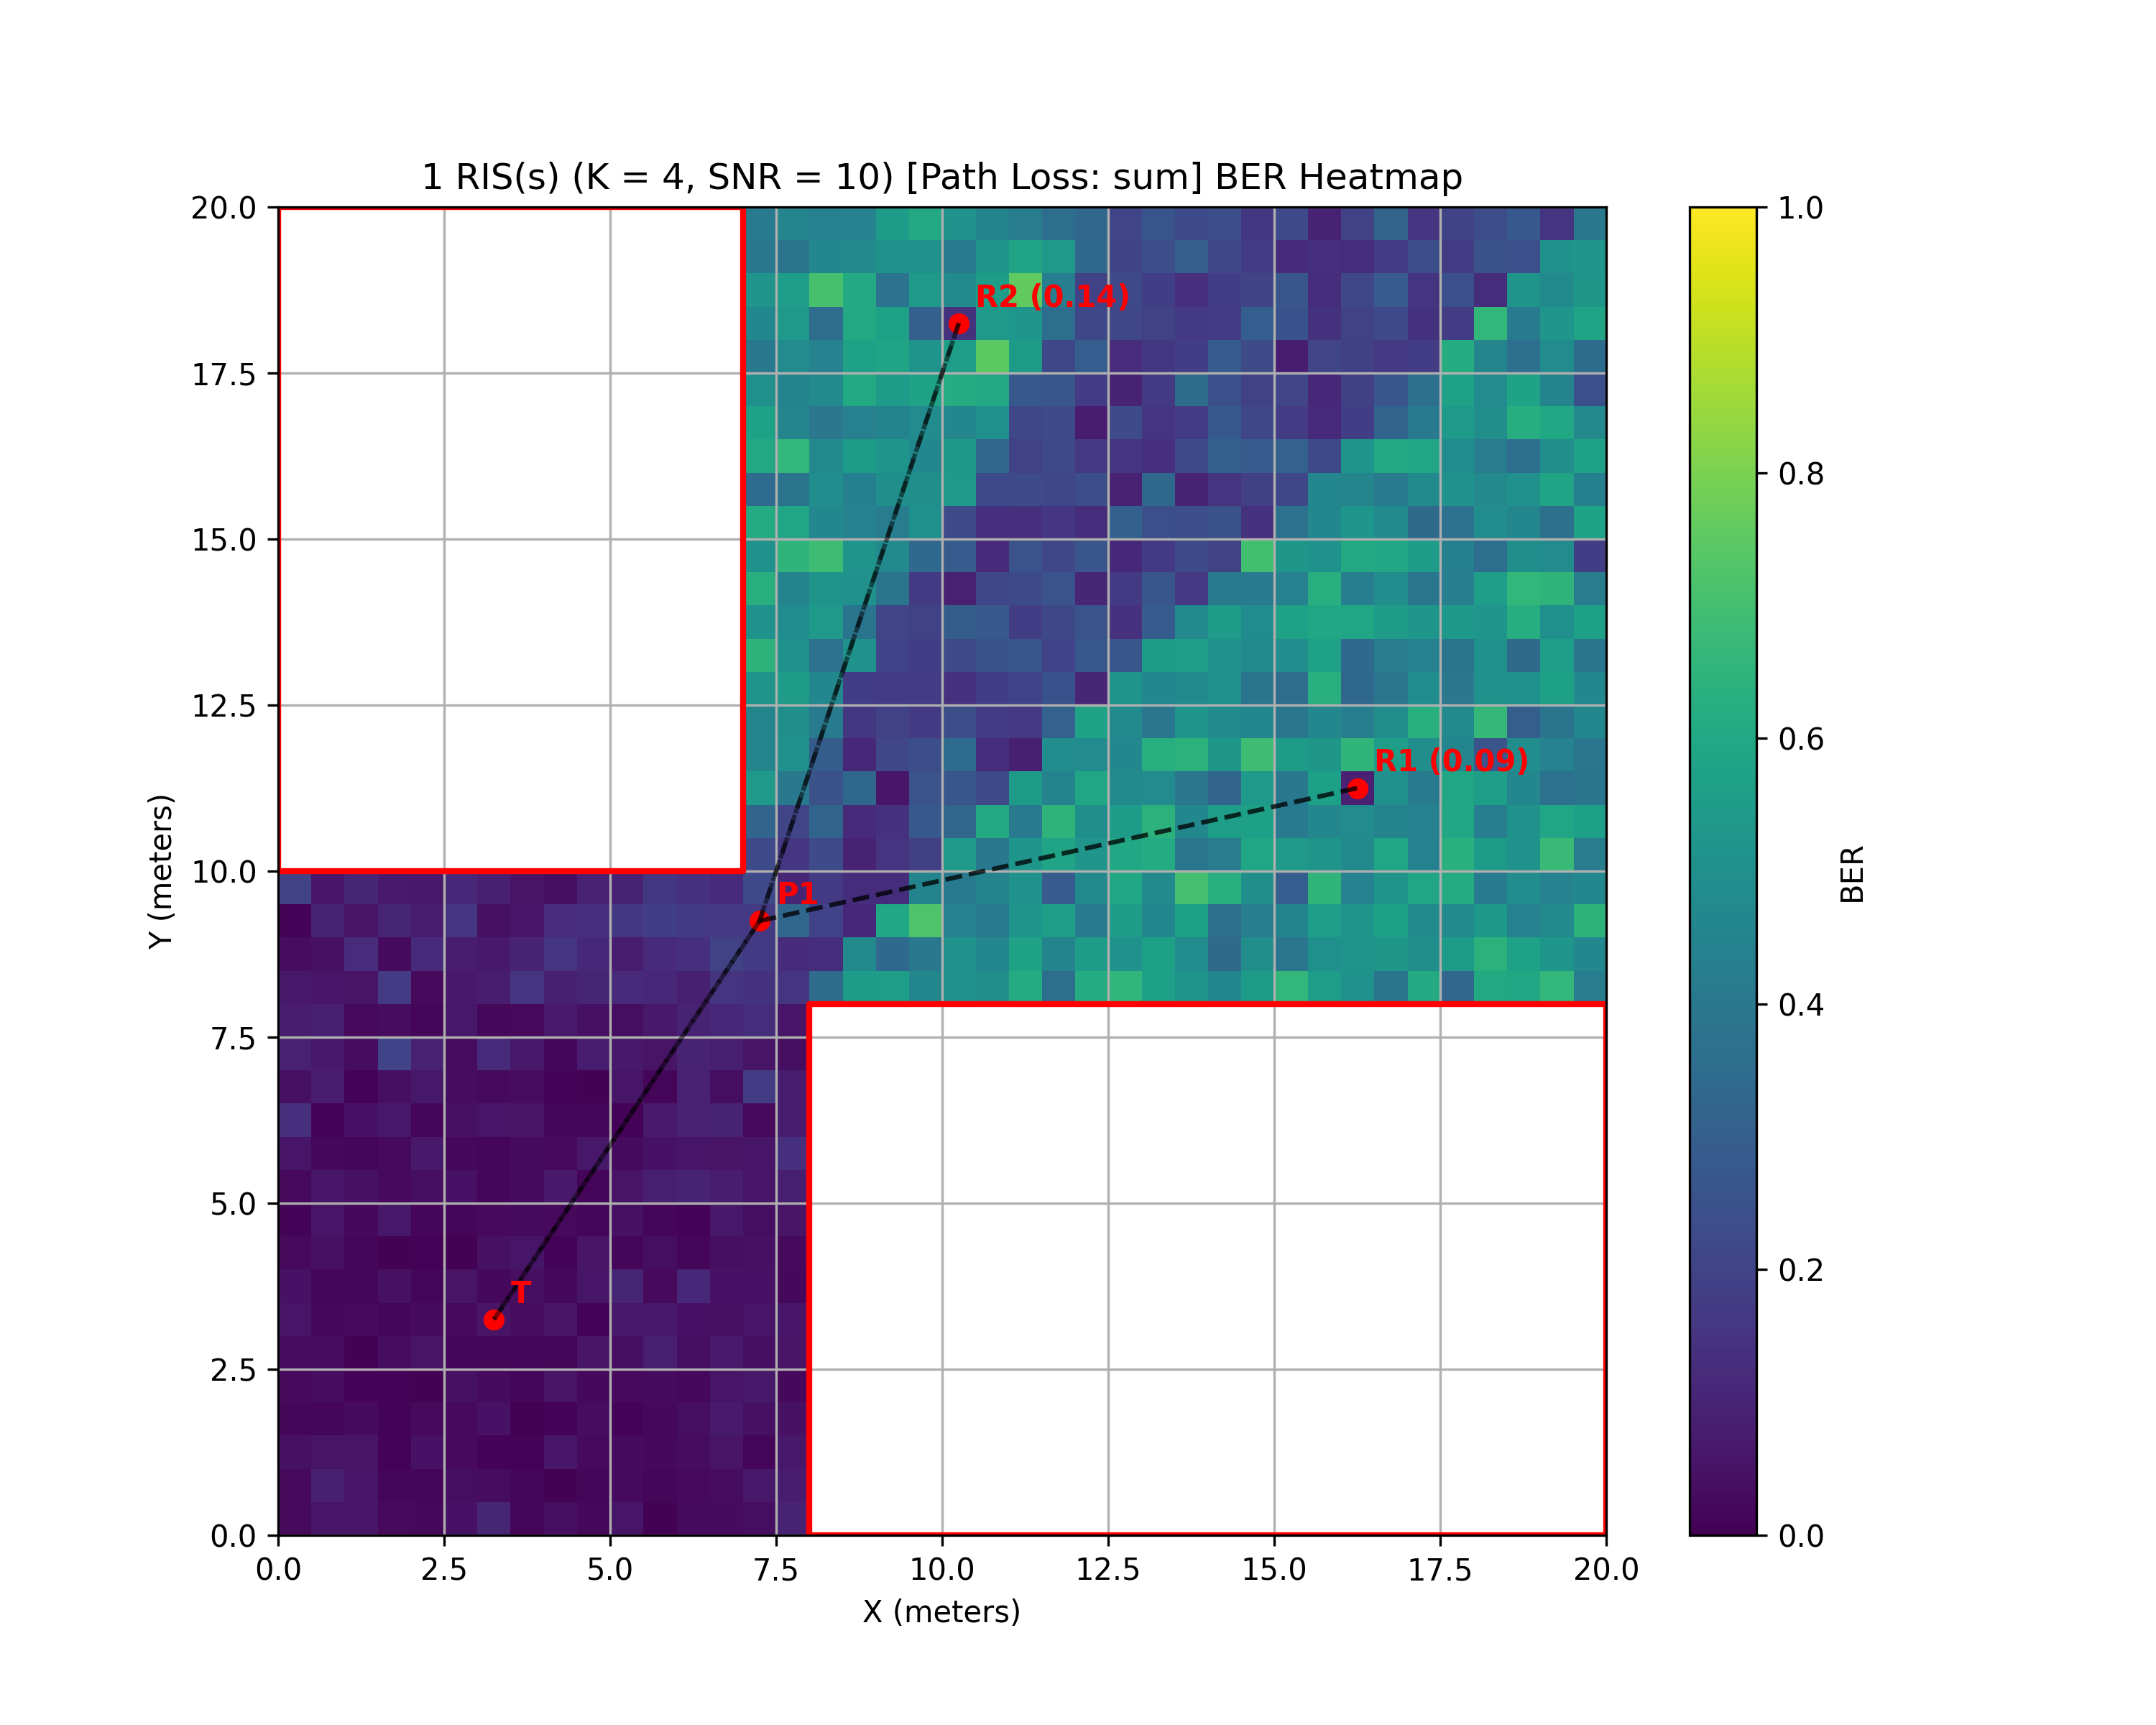
\includegraphics[width=\textwidth]{imgs/heatmap-simulations/1 RIS(s) (K = 4, SNR = 10) [Path Loss_ sum] BER Heatmap.png}
    \caption{BER Heatmap}
  \end{subfigure}
  \hfill
  \begin{subfigure}[b]{0.48\textwidth}
    \centering
    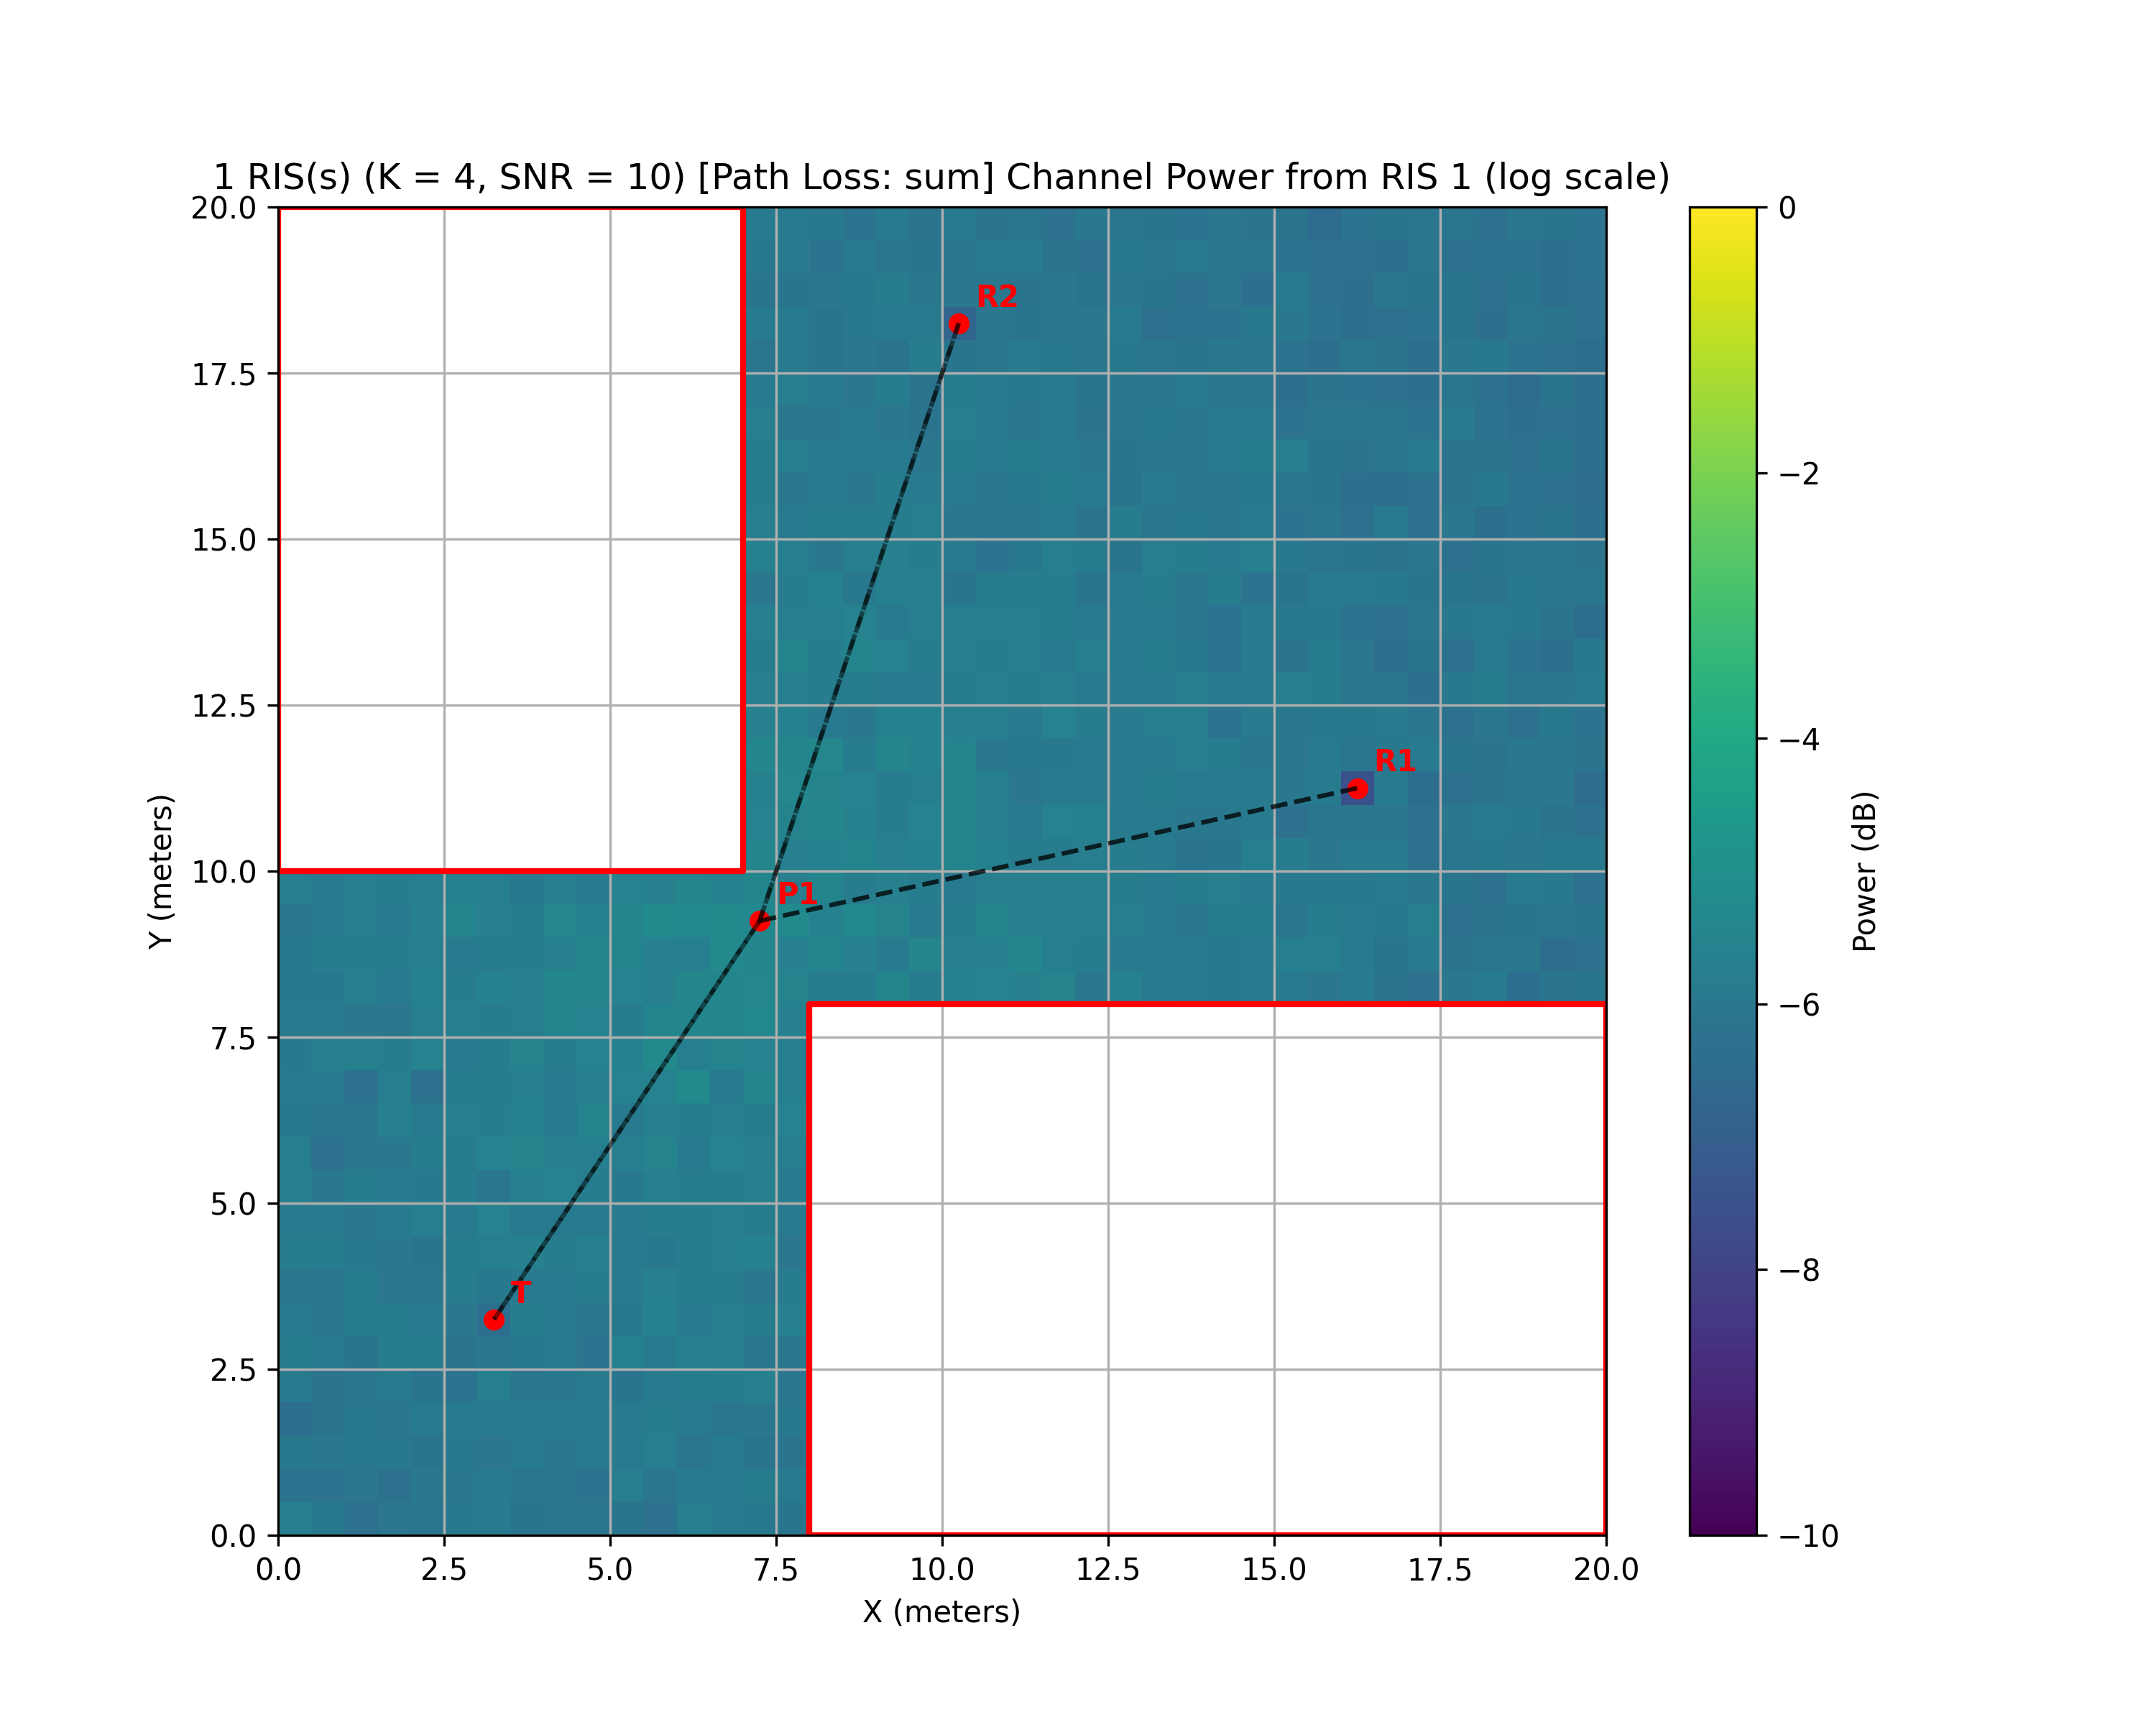
\includegraphics[width=\textwidth]{imgs/heatmap-simulations/1 RIS(s) (K = 4, SNR = 10) [Path Loss_ sum] Channel Power from RIS 1 (log scale).png}
    \caption{Channel Power from RIS 1 (log scale)}
  \end{subfigure}
  \caption{1 RIS(s) [Path Loss: sum] }
\end{figure}

\subsubsection{Double reflection from 2 RIS in series}

It is certainly interesting to also study what would happen if we concatenate two RIS in series in relation to their combined path loss. For these tests, we used $\lambda = 0.08m, \tau = 0.6, \xi = 1, \eta = 0.9, SNR = 10dB, K = 2, N = 16$.

All scenarios suppose the RIS use the same kind of path loss, meaning they are of different kind (active, passive uniform, passive directional). Of course, it would be an interesting case studying combining different variations of them to reach the most cost and power - efficient configuration.

Additional scenarios with RIS in parallel would also be valuable for future research, as they would likely show promising security characteristics based on our preliminary analysis.

\paragraph*{Path loss: active}
Similar to the previous scenario, we can clearly see where the RIS have significant power to influence the signal reception, and where without LOS the signal is undecipherable for eavesdroppers.

As said before, it is slightly visible where the direct signal from \textbf{T} is and is not present. It is not visible however the difference where only \textbf{P2} creates interference from where both \textbf{P1} and \textbf{P2} contribute to the noise. You could imagine the area by selecting the intersection between the two RIS Channel Power graphs.

\begin{figure}[H]
  \centering
  \begin{subfigure}[b]{0.48\textwidth}
    \centering
    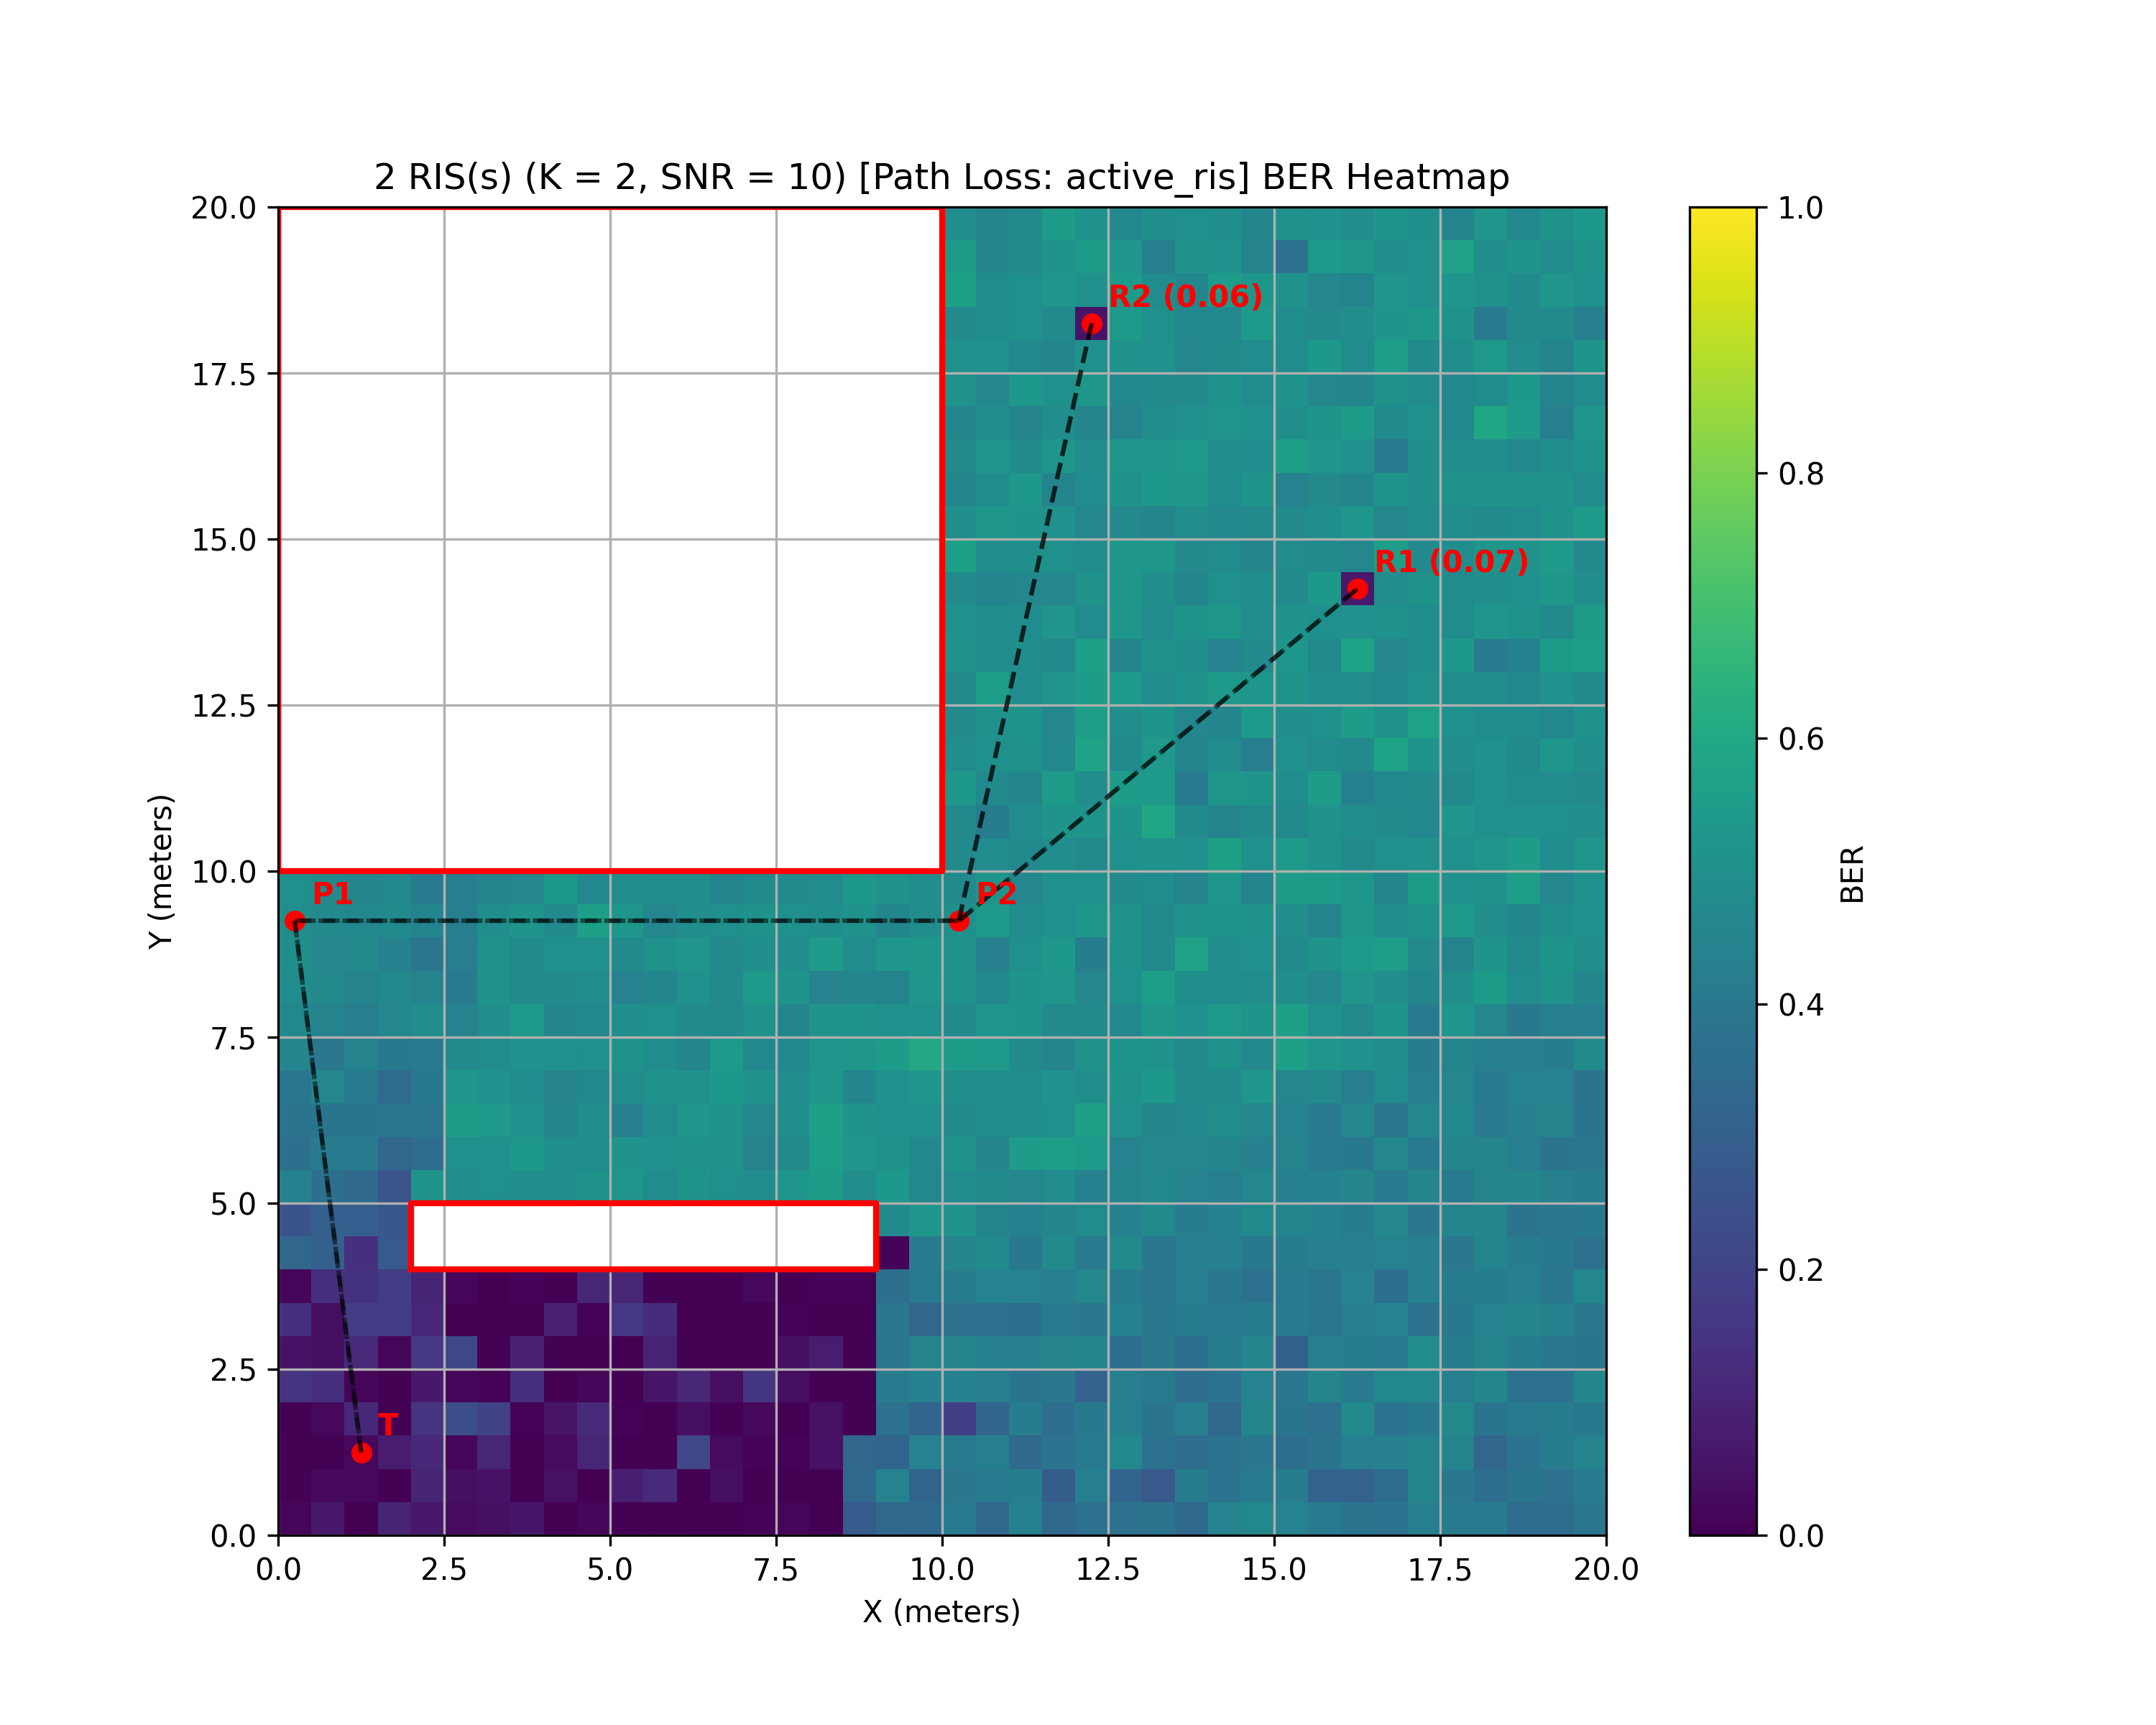
\includegraphics[width=\textwidth]{imgs/heatmap-simulations/2 RIS(s) (K = 2, SNR = 10) [Path Loss_ active_ris] BER Heatmap.png}
    \caption{BER Heatmap}
  \end{subfigure}
  \hfill
  \begin{subfigure}[b]{0.48\textwidth}
    \centering
    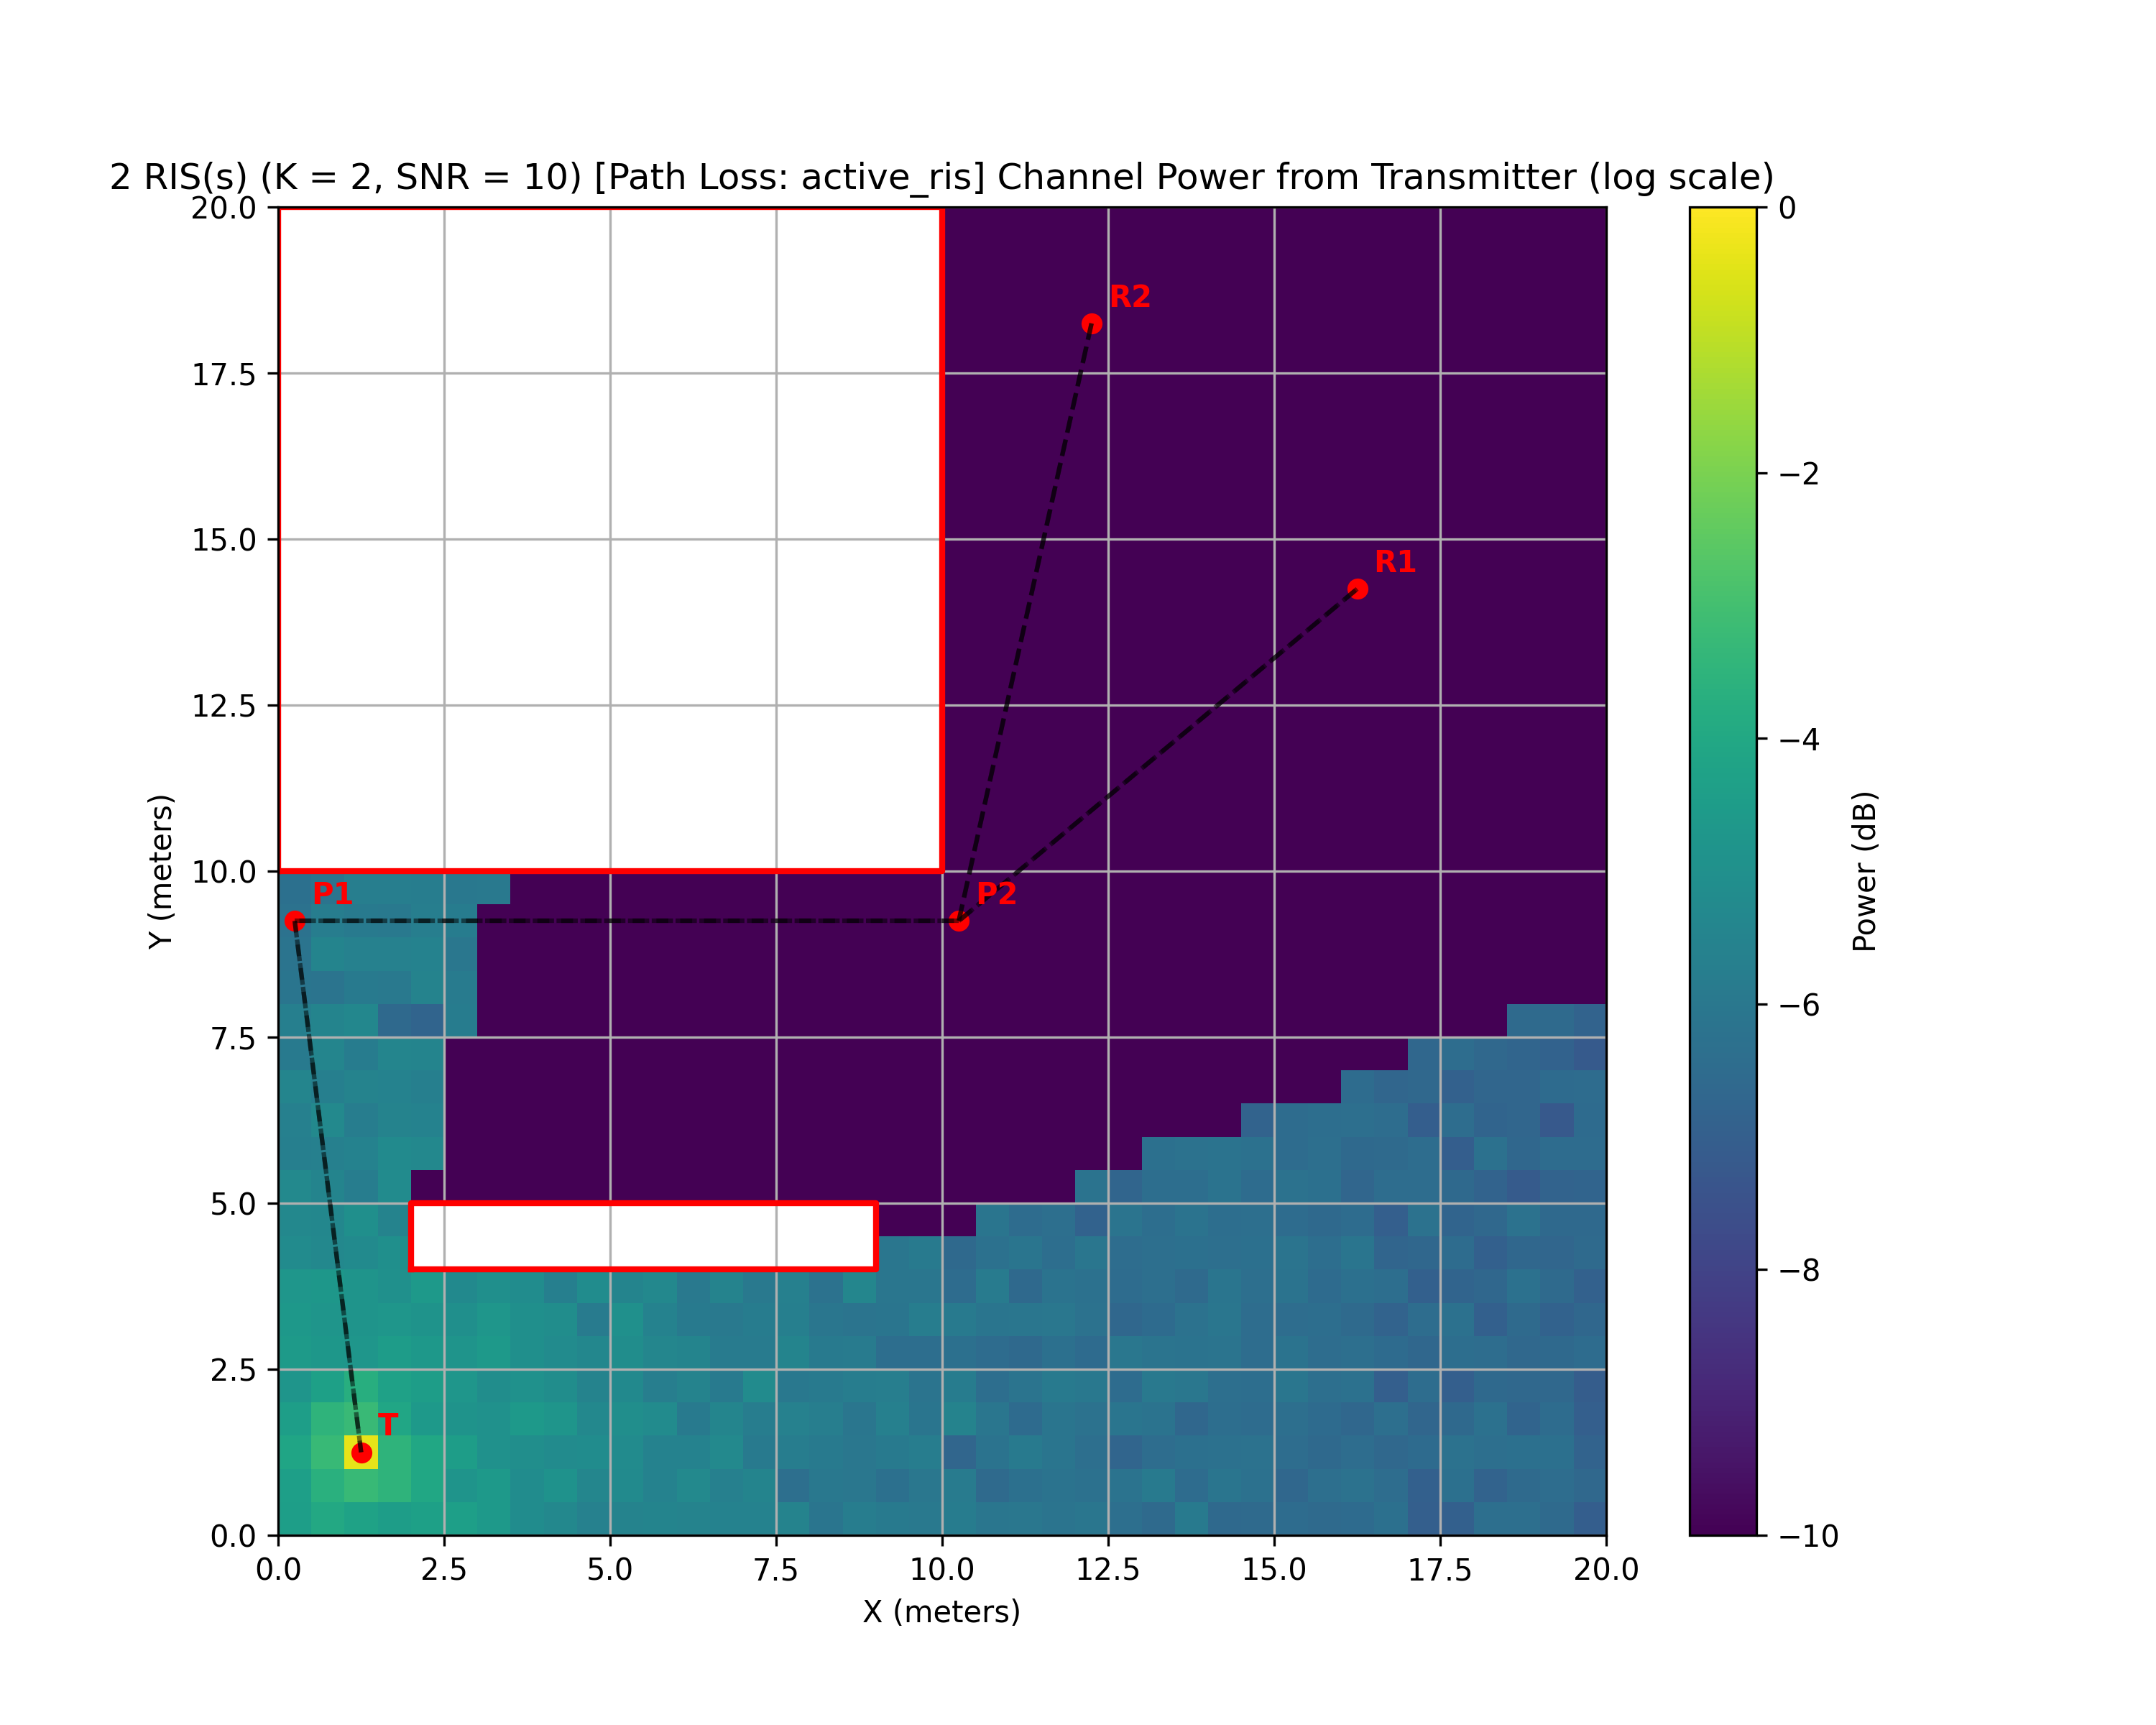
\includegraphics[width=\textwidth]{imgs/heatmap-simulations/2 RIS(s) (K = 2, SNR = 10) [Path Loss_ active_ris] Channel Power from Transmitter (log scale).png}
    \caption{Channel Power from Transmitter (log scale)}
  \end{subfigure}
  \medskip
  \centering
  \begin{subfigure}[b]{0.48\textwidth}
    \centering
    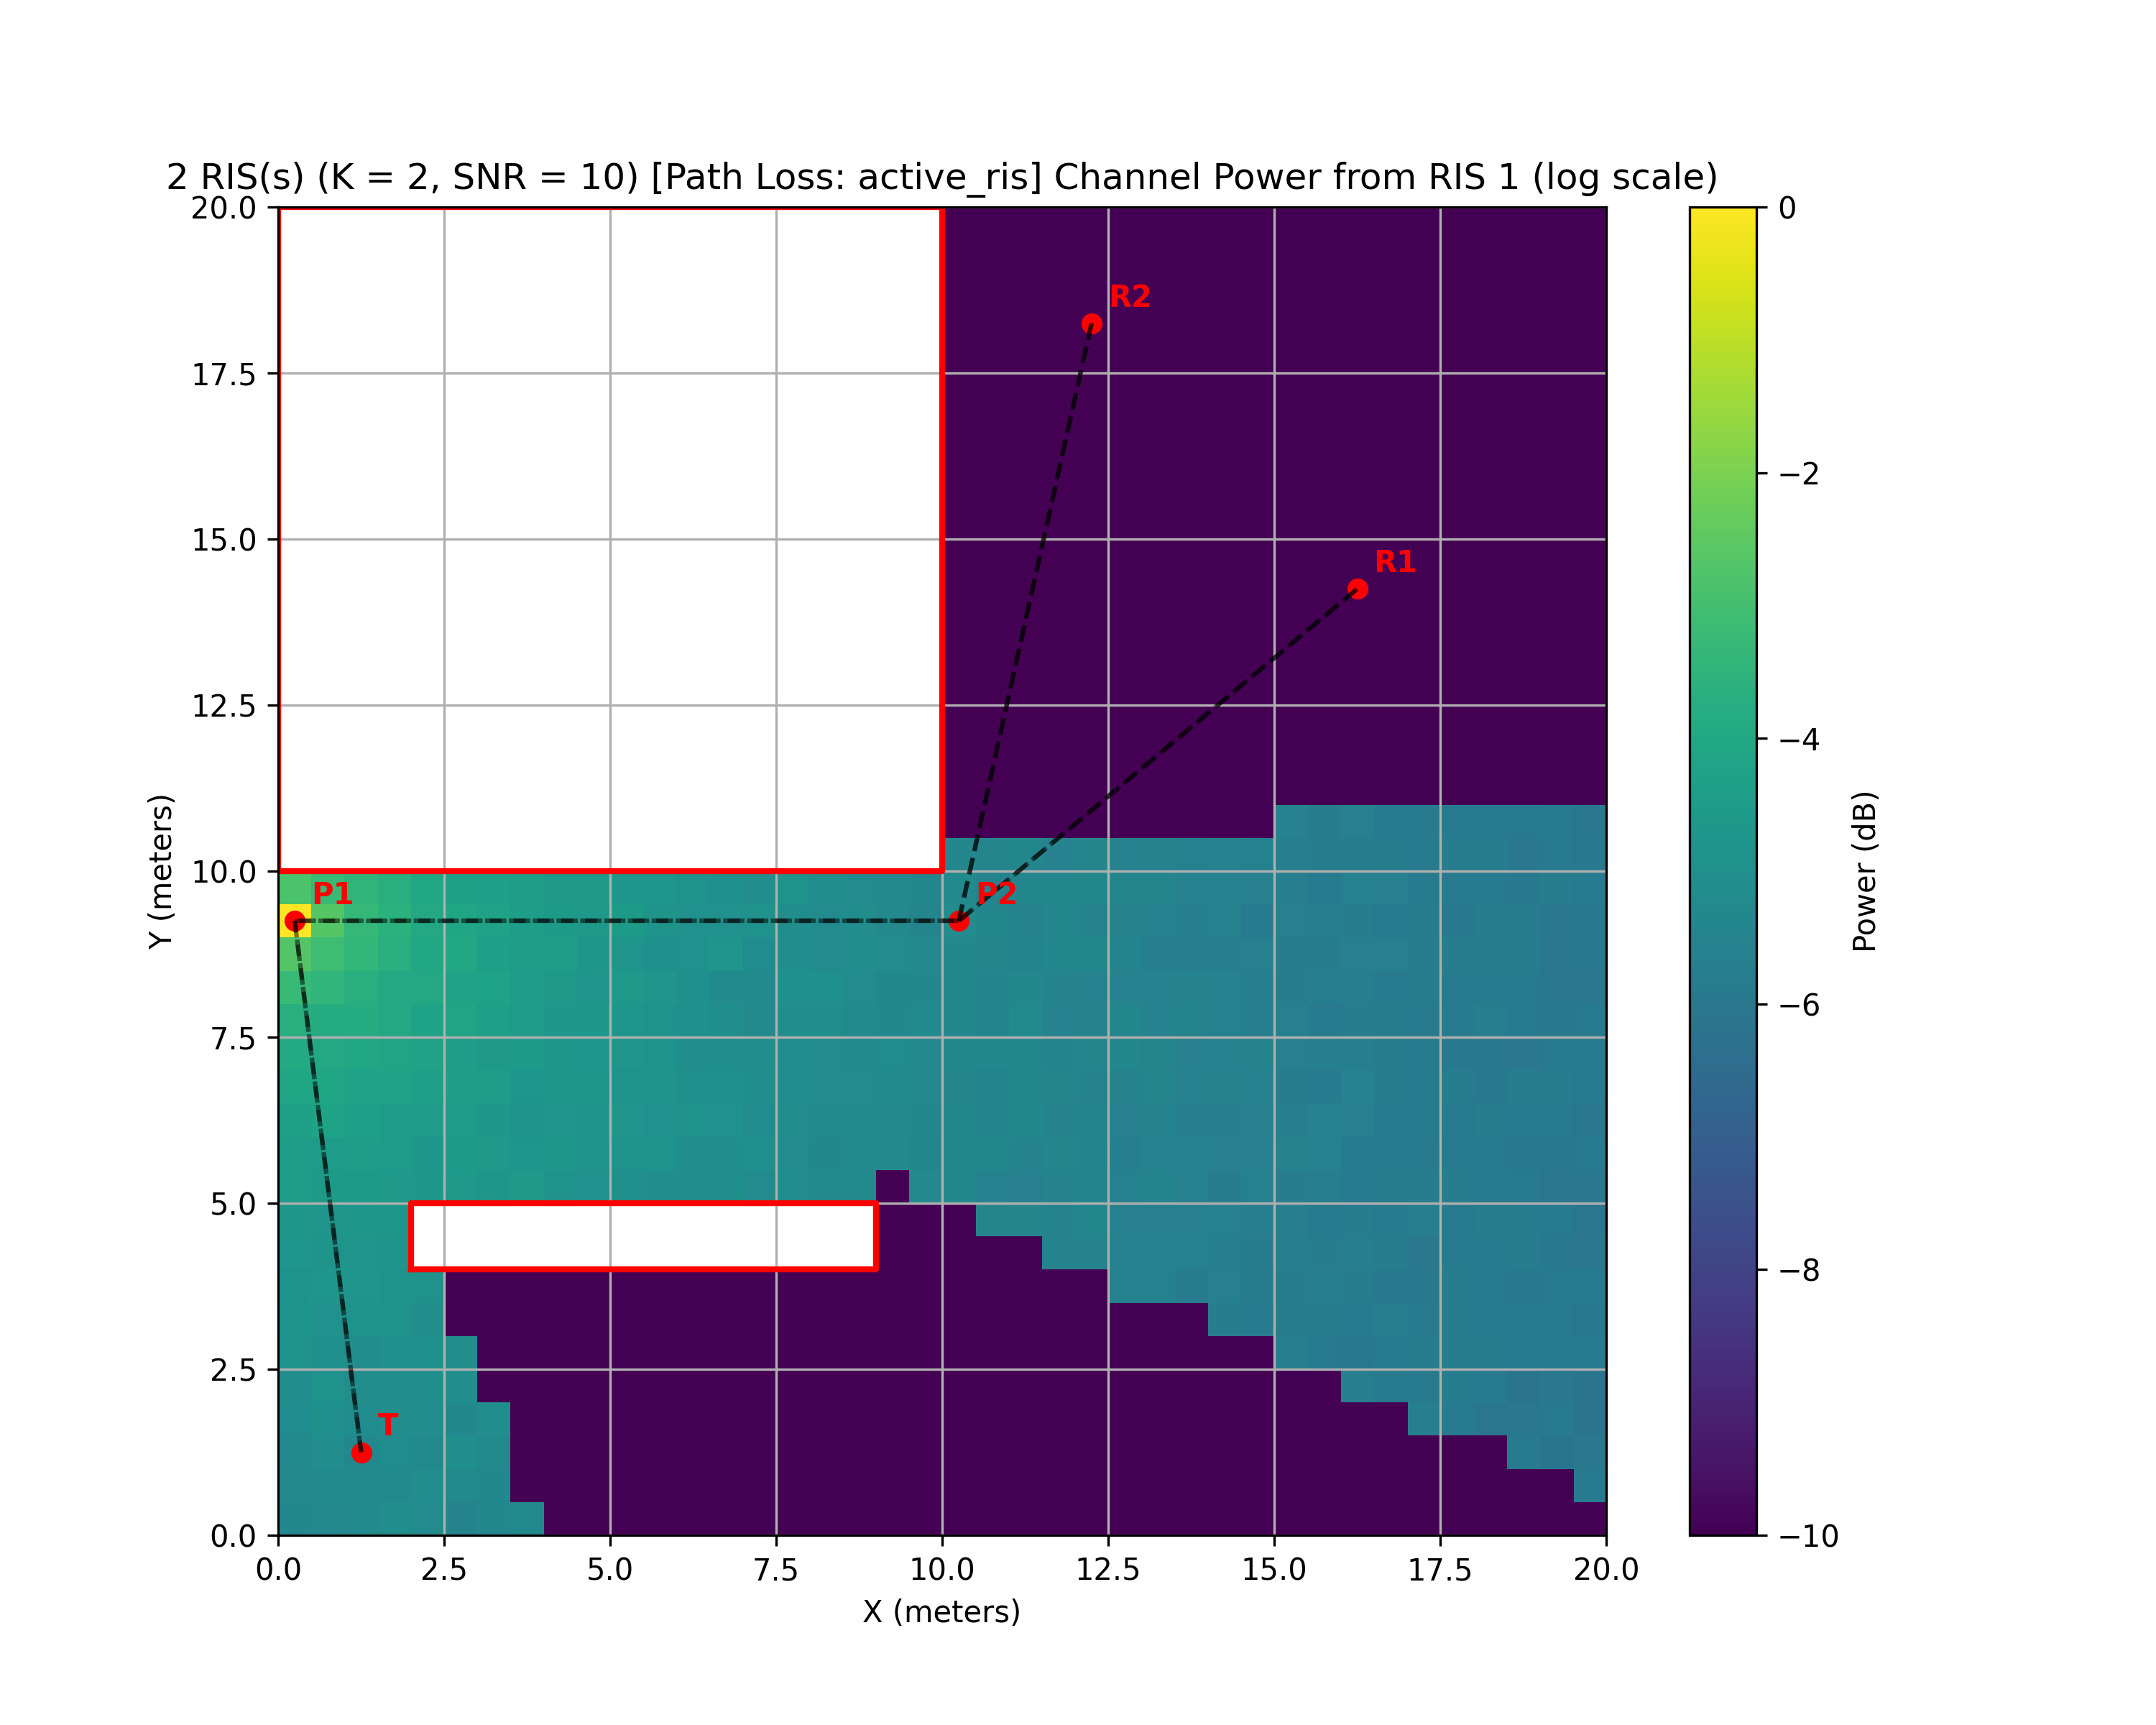
\includegraphics[width=\textwidth]{imgs/heatmap-simulations/2 RIS(s) (K = 2, SNR = 10) [Path Loss_ active_ris] Channel Power from RIS 1 (log scale).png}
    \caption{Channel Power from RIS 1 (log scale)}
  \end{subfigure}
  \hfill
  \begin{subfigure}[b]{0.48\textwidth}
    \centering
    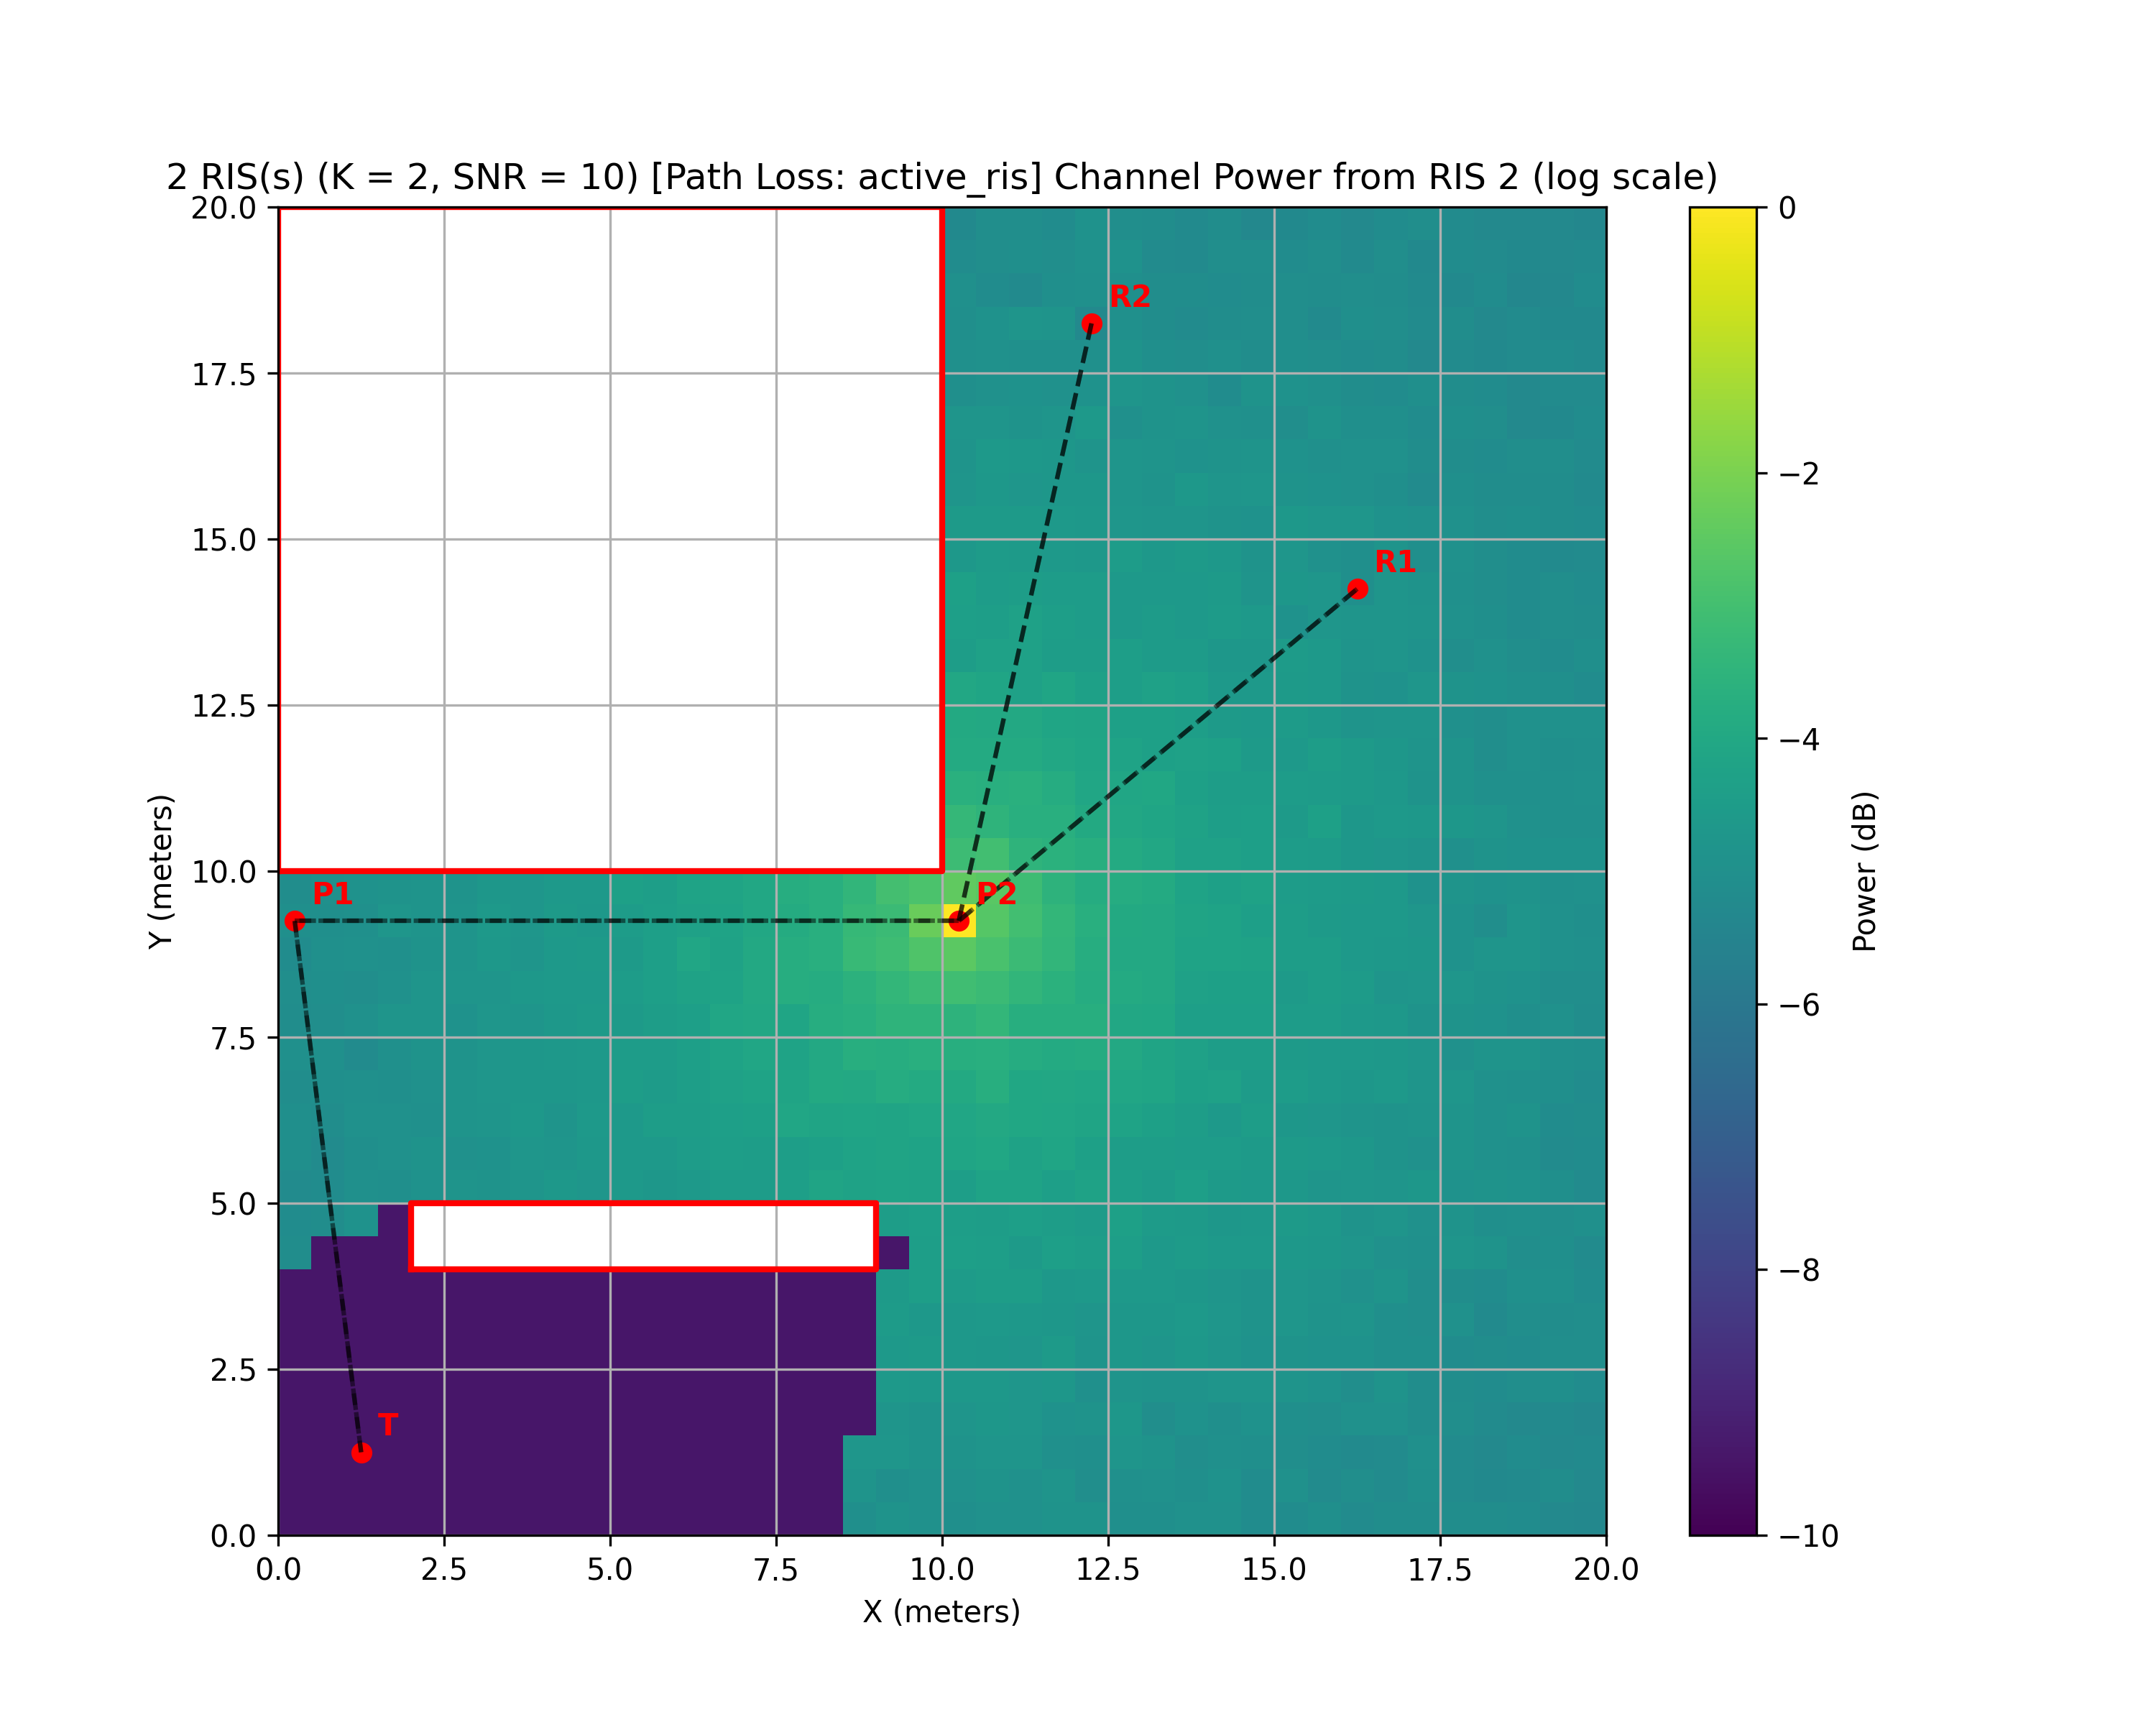
\includegraphics[width=\textwidth]{imgs/heatmap-simulations/2 RIS(s) (K = 2, SNR = 10) [Path Loss_ active_ris] Channel Power from RIS 2 (log scale).png}
    \caption{Channel Power from RIS 2 (log scale)}
  \end{subfigure}
  \caption{2 RIS(s) [Path Loss: active ris]}
\end{figure}

\paragraph*{Path loss: product}
We can draw similar conclusions as before for the product path loss. As we can see, the direct signal is not disturbed, and the reflection from \textbf{P2} after being already reflected from \textbf{P1} is so low, it does not even show on the \textbf{P2} position itself.

\begin{figure}[H]
  \centering
  \begin{subfigure}[b]{0.48\textwidth}
    \centering
    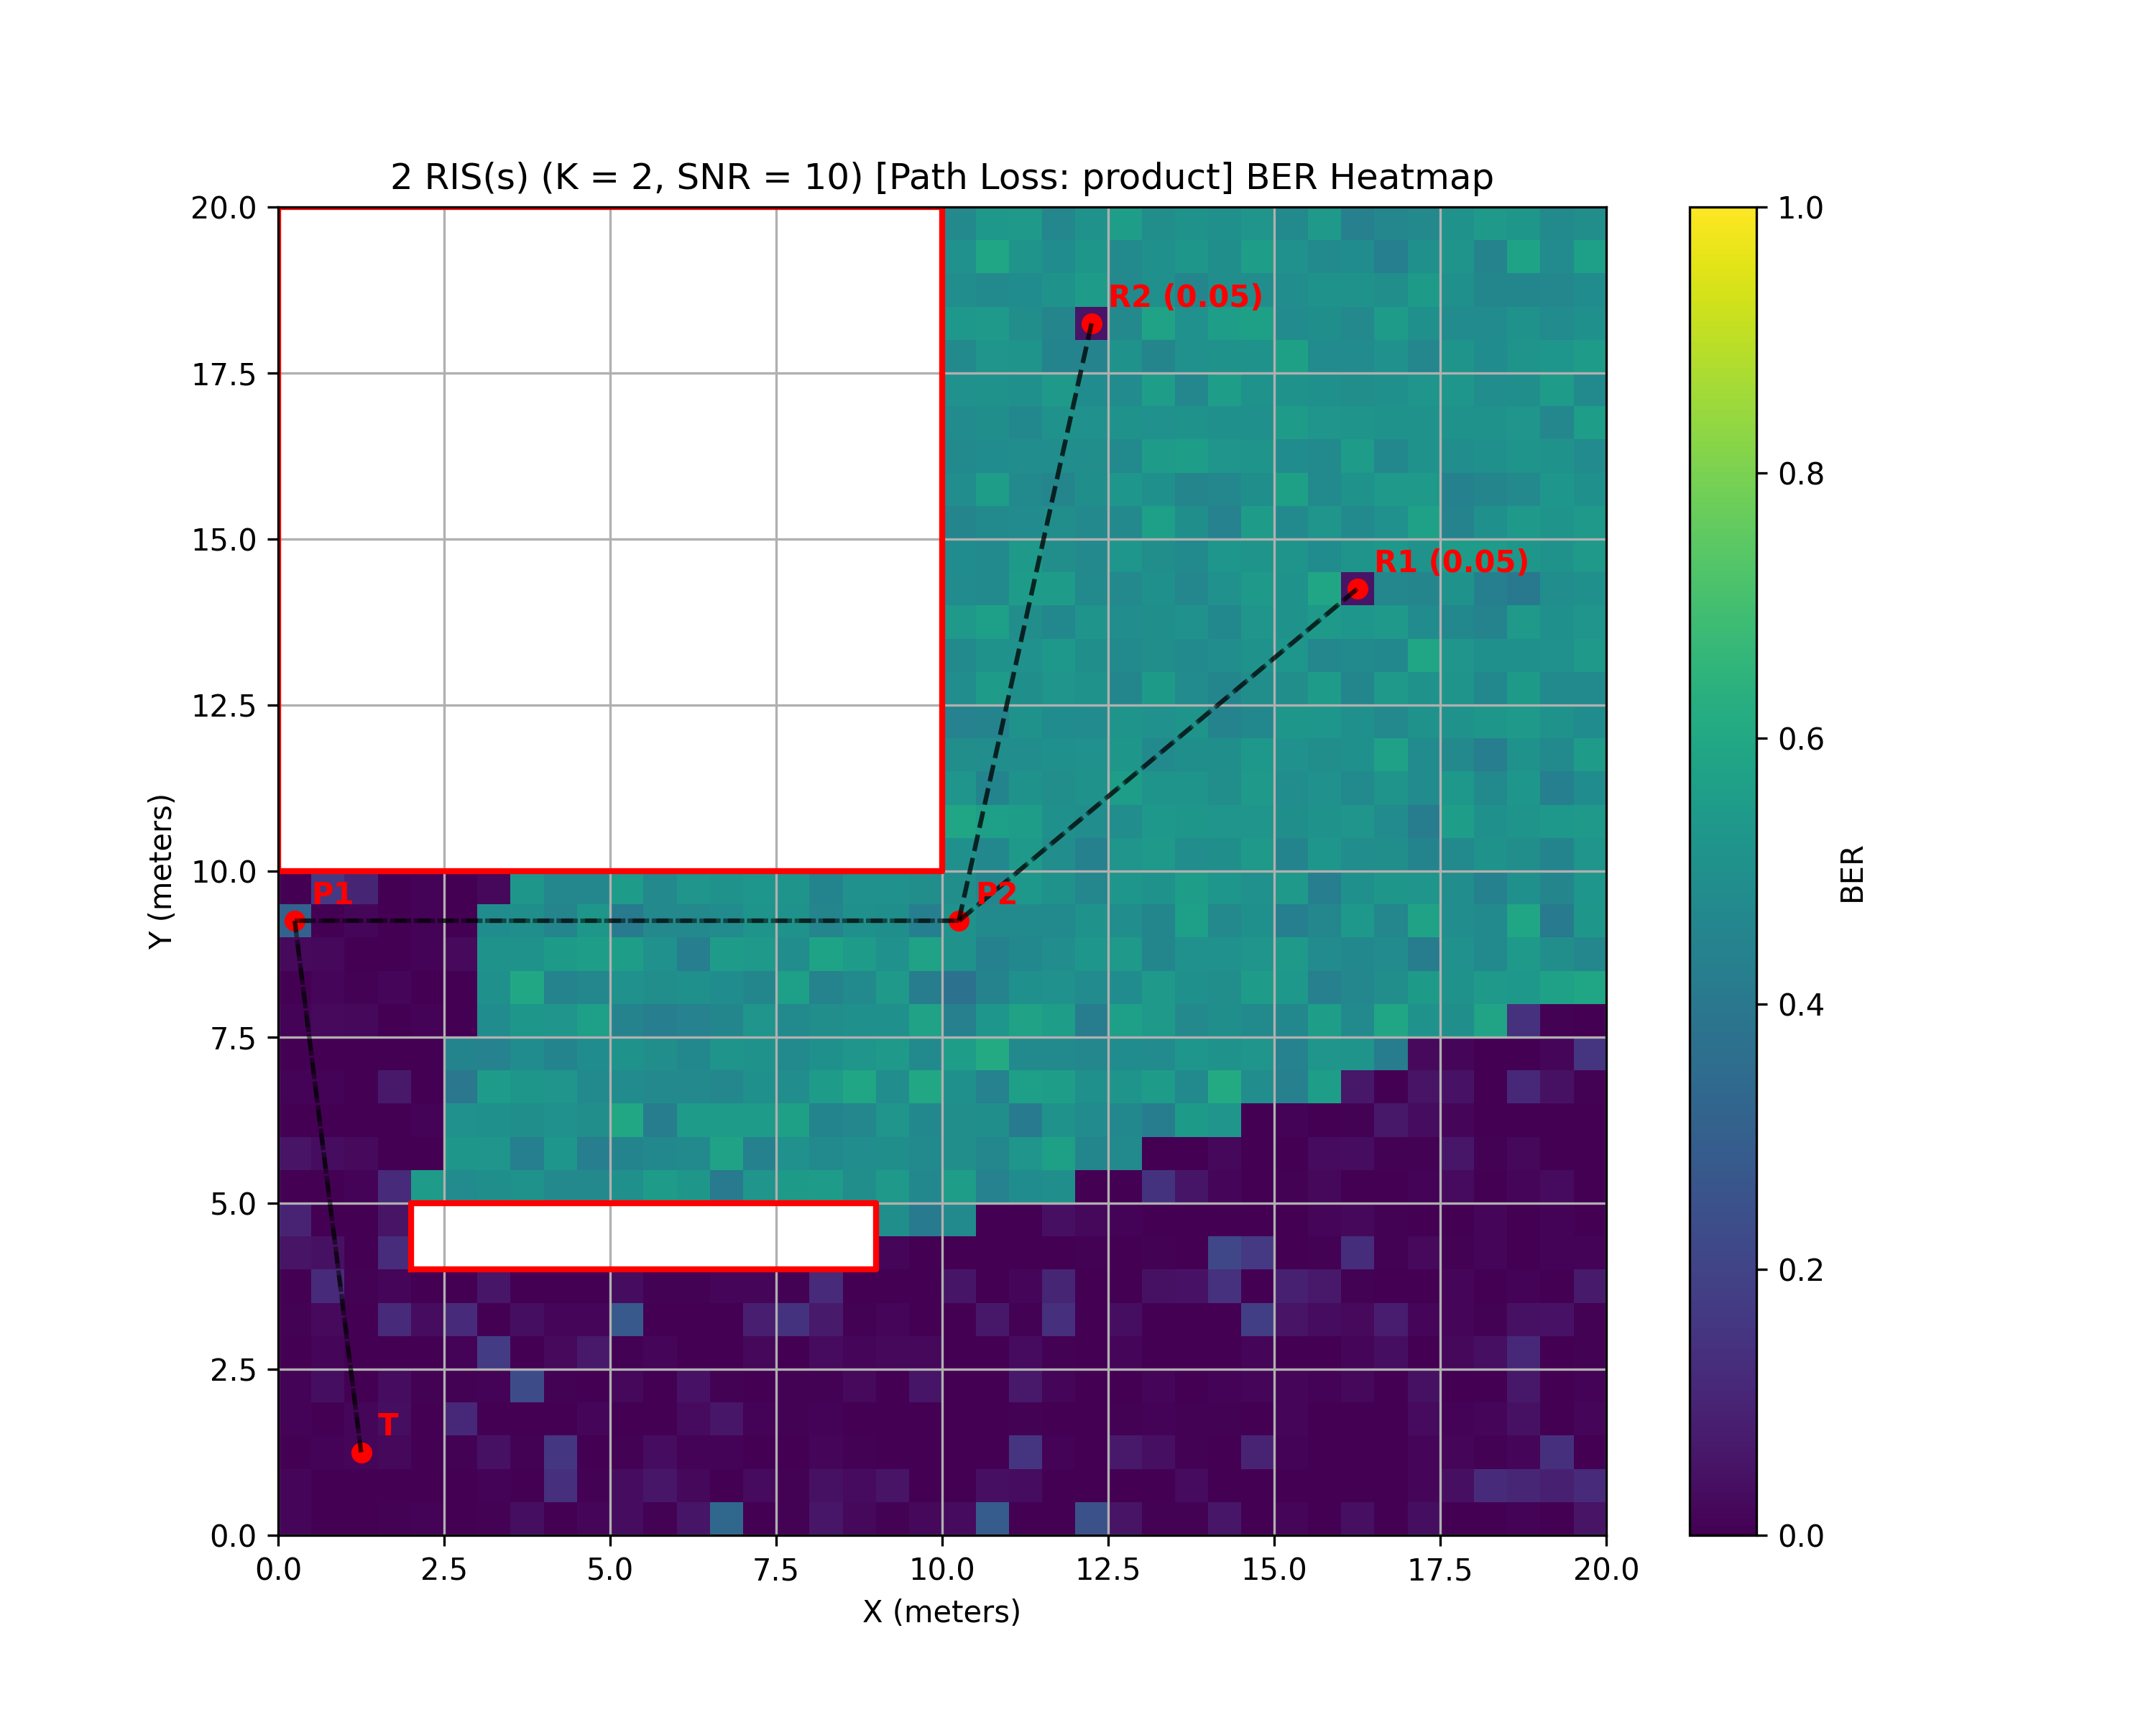
\includegraphics[width=\textwidth]{imgs/heatmap-simulations/2 RIS(s) (K = 2, SNR = 10) [Path Loss_ product] BER Heatmap.png}
    \caption{BER Heatmap}
  \end{subfigure}
  \hfill
  \begin{subfigure}[b]{0.48\textwidth}
    \centering
    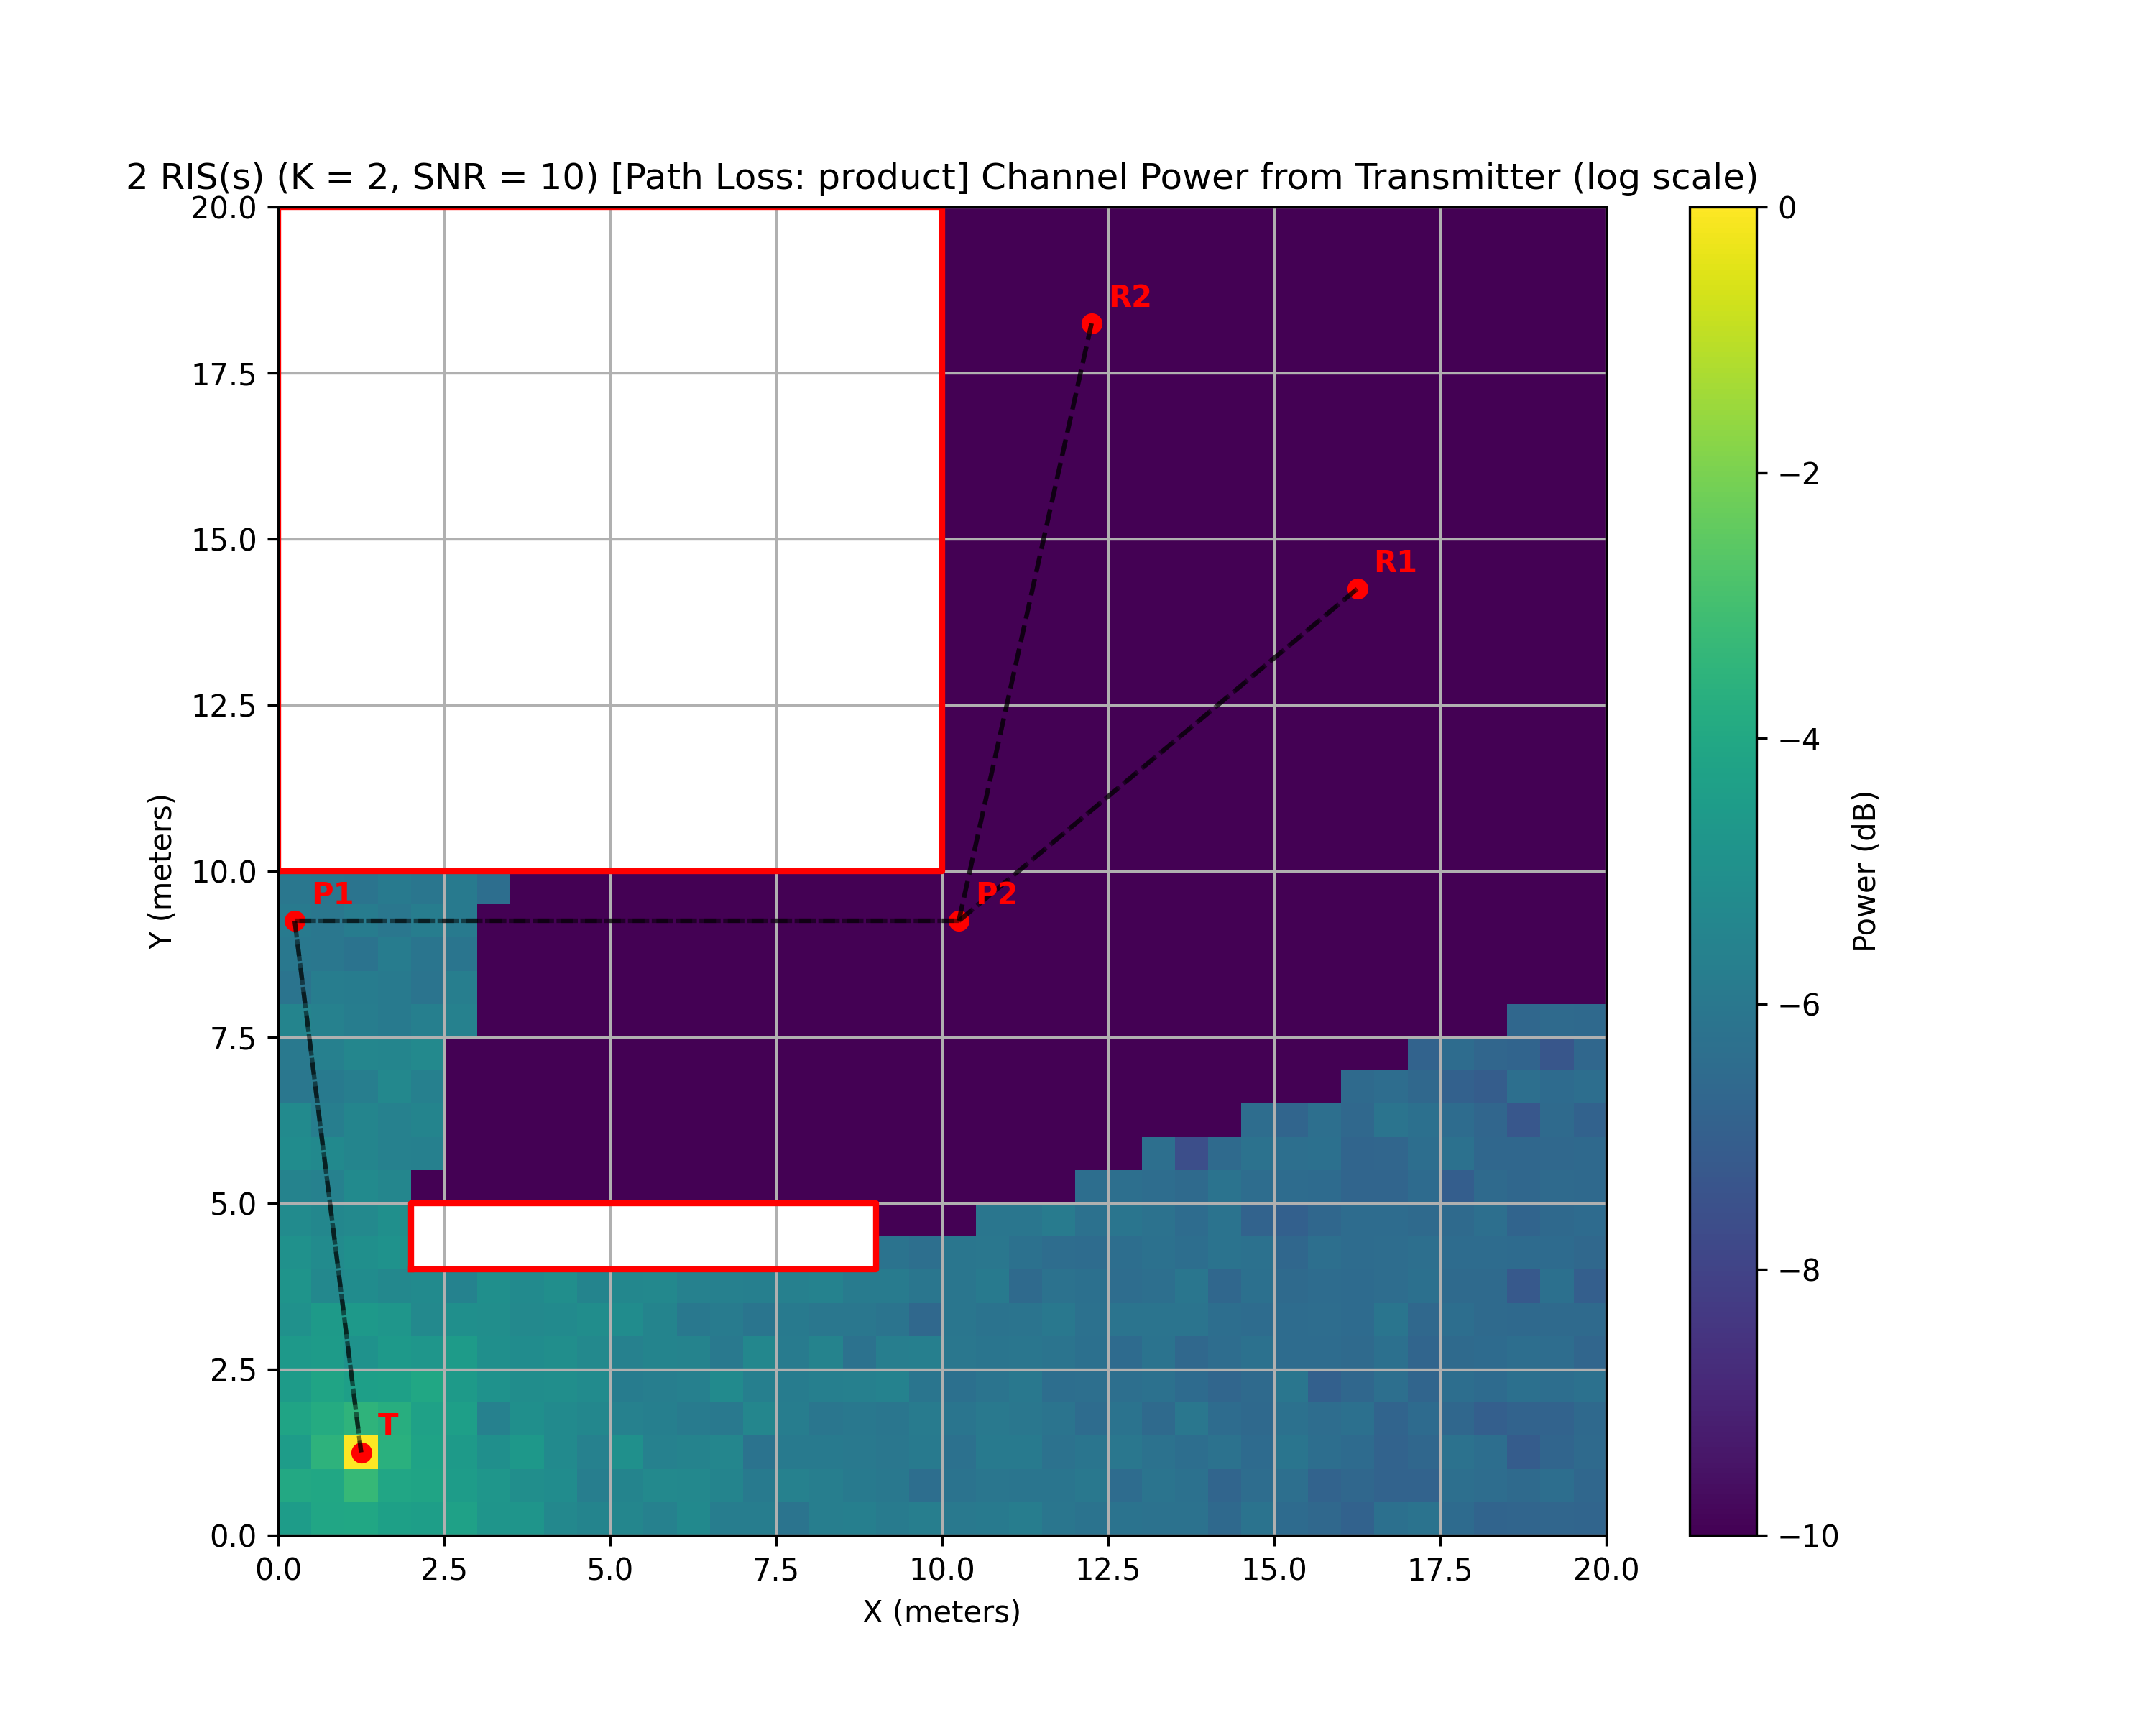
\includegraphics[width=\textwidth]{imgs/heatmap-simulations/2 RIS(s) (K = 2, SNR = 10) [Path Loss_ product] Channel Power from Transmitter (log scale).png}
    \caption{Channel Power from Transmitter (log scale)}
  \end{subfigure}
  \caption{2 RIS(s) [Path Loss: product]}
  \medskip
  \centering
  \begin{subfigure}[b]{0.48\textwidth}
    \centering
    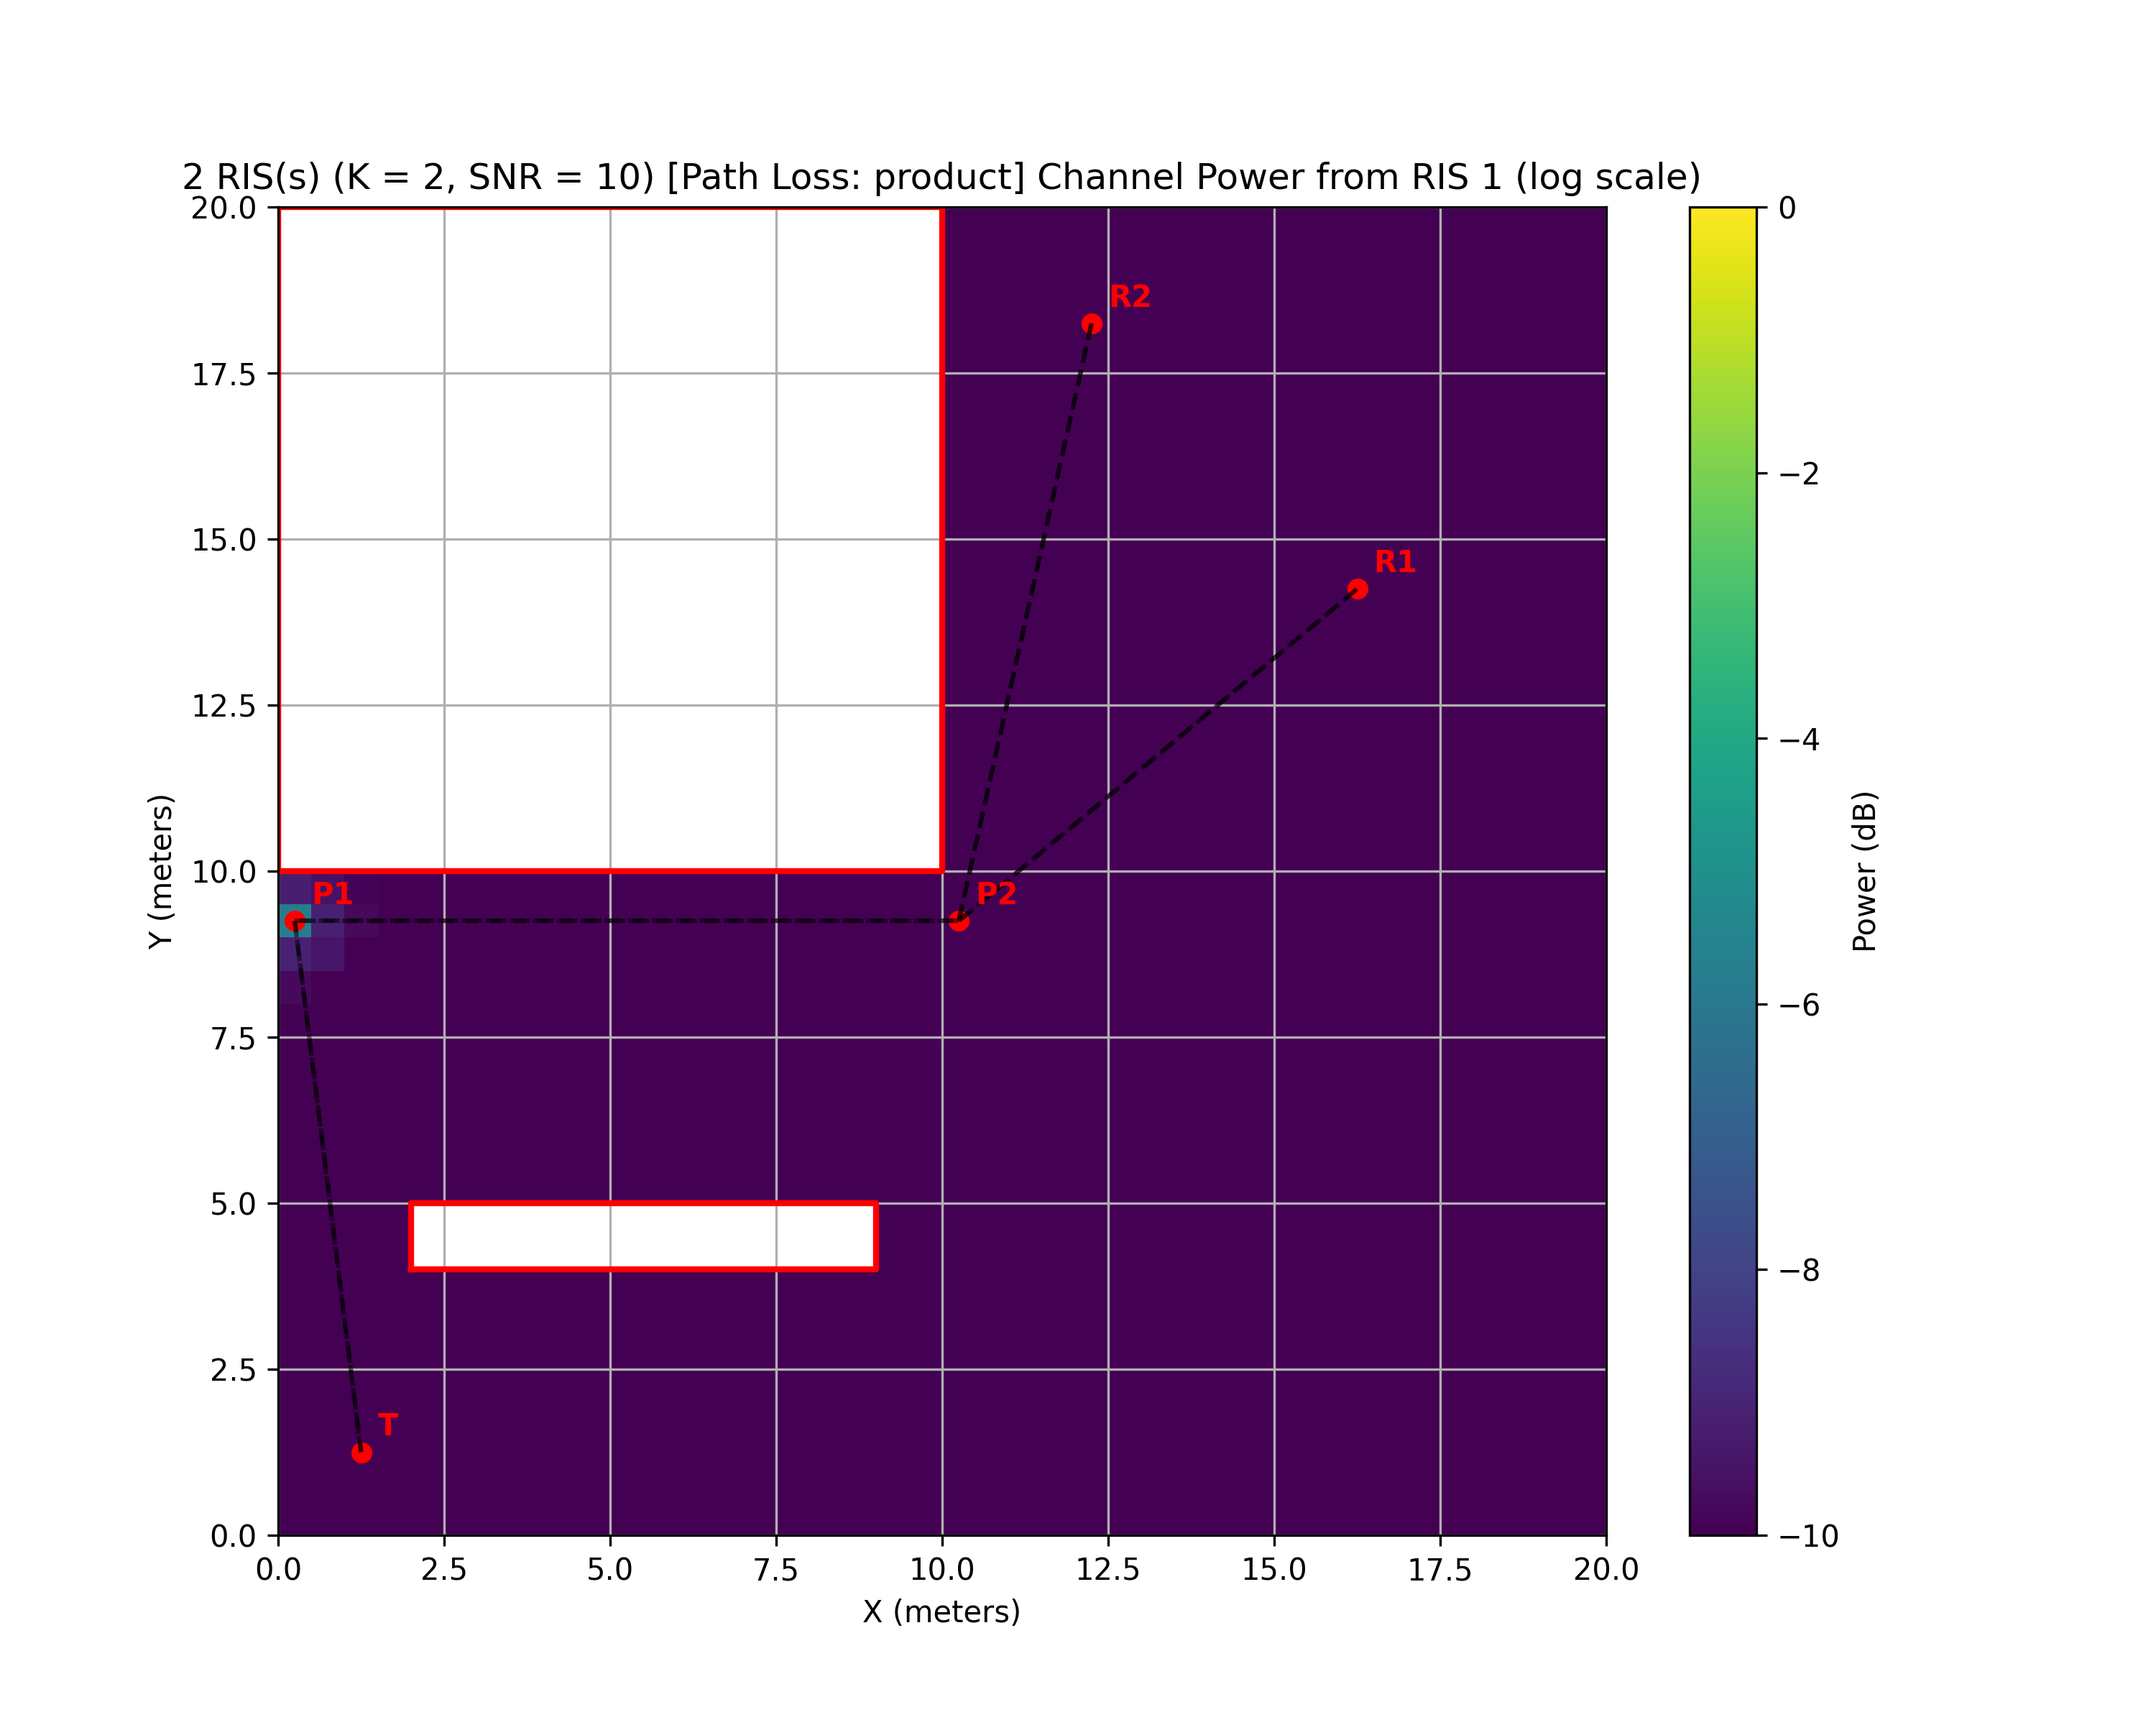
\includegraphics[width=\textwidth]{imgs/heatmap-simulations/2 RIS(s) (K = 2, SNR = 10) [Path Loss_ product] Channel Power from RIS 1 (log scale).png}
    \caption{Channel Power from RIS 1 (log scale)}
  \end{subfigure}
  \hfill
  \begin{subfigure}[b]{0.48\textwidth}
    \centering
    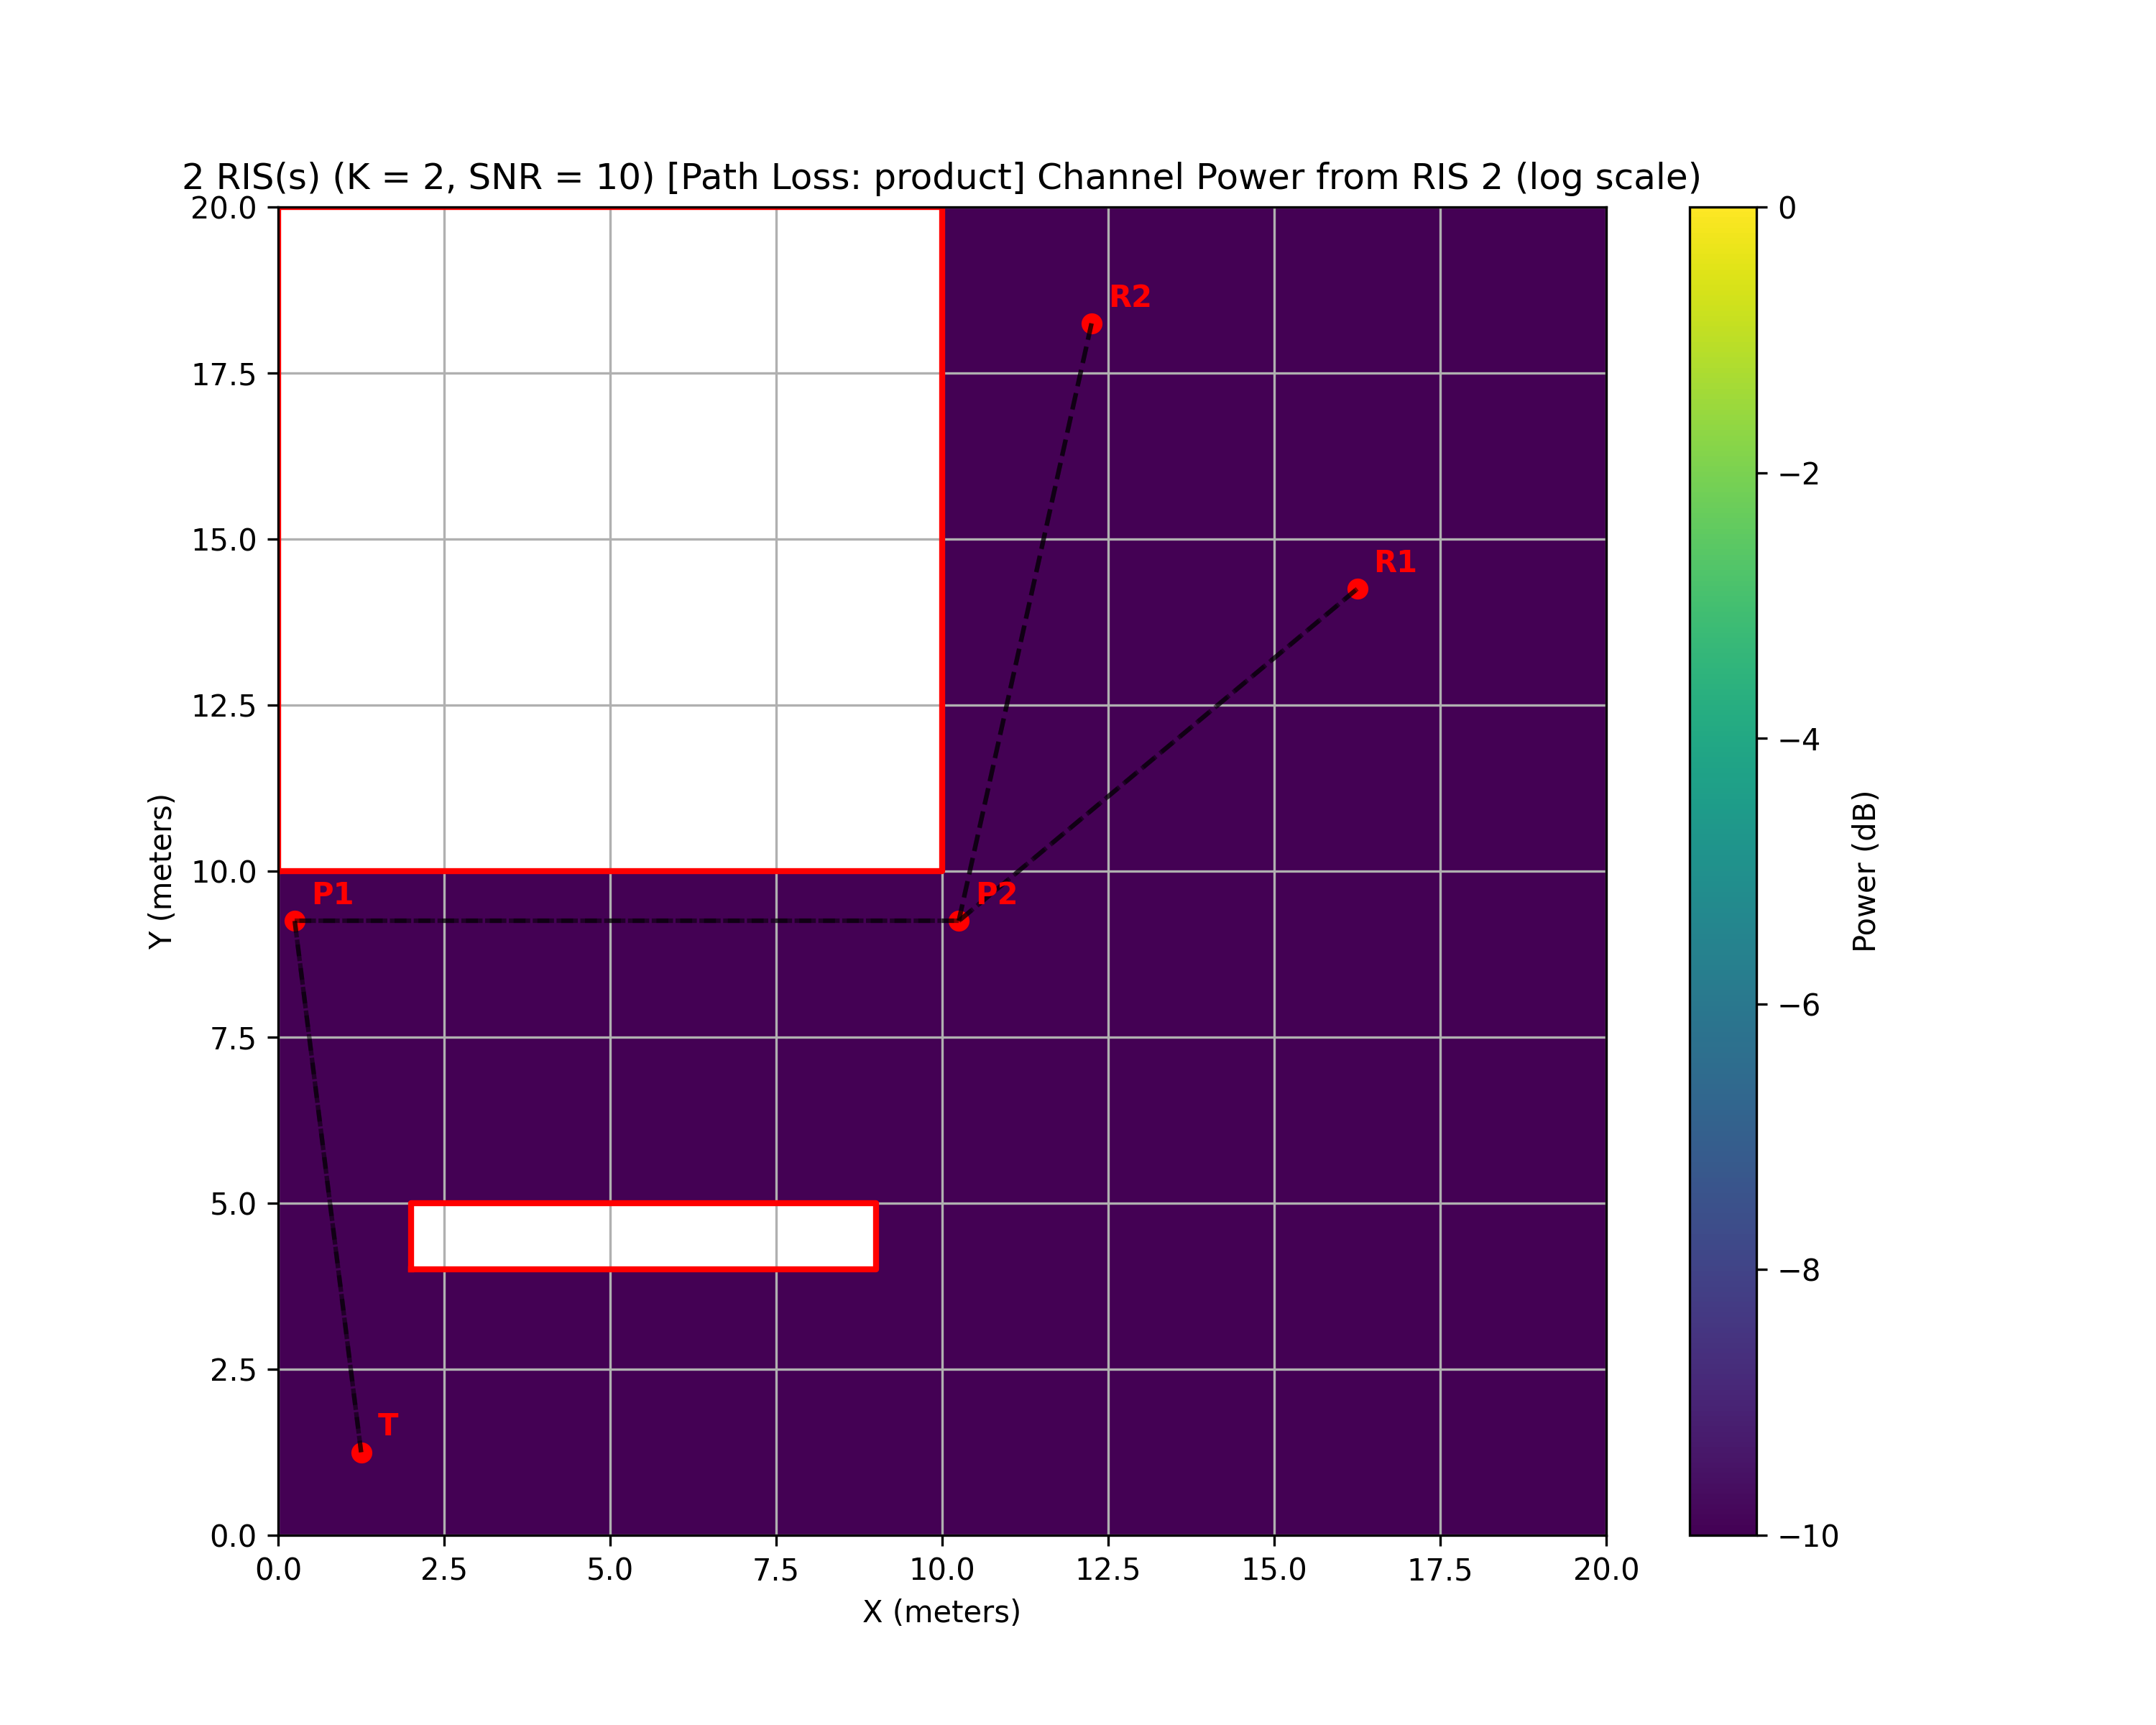
\includegraphics[width=\textwidth]{imgs/heatmap-simulations/2 RIS(s) (K = 2, SNR = 10) [Path Loss_ product] Channel Power from RIS 2 (log scale).png}
    \caption{Channel Power from RIS 2 (log scale)}
  \end{subfigure}
  \caption{2 RIS(s) [Path Loss: product]}
\end{figure}

\paragraph*{Path loss: sum}
The distinction between having or not LOS are very visible here. The displayed values for the BER are in line with the previous graph on the same kind of path loss.

Like the active path loss, here there is no difference in having a single disturbance from \textbf{P2} versus from both \textbf{P1} and \textbf{P2}.

We do remember also here that this graph is not realistic, as RIS should be directional. Again, we invite you to consider this as the sum of all possible direction the RIS could take.

\begin{figure}[H]
  \centering
  \begin{subfigure}[b]{0.48\textwidth}
    \centering
    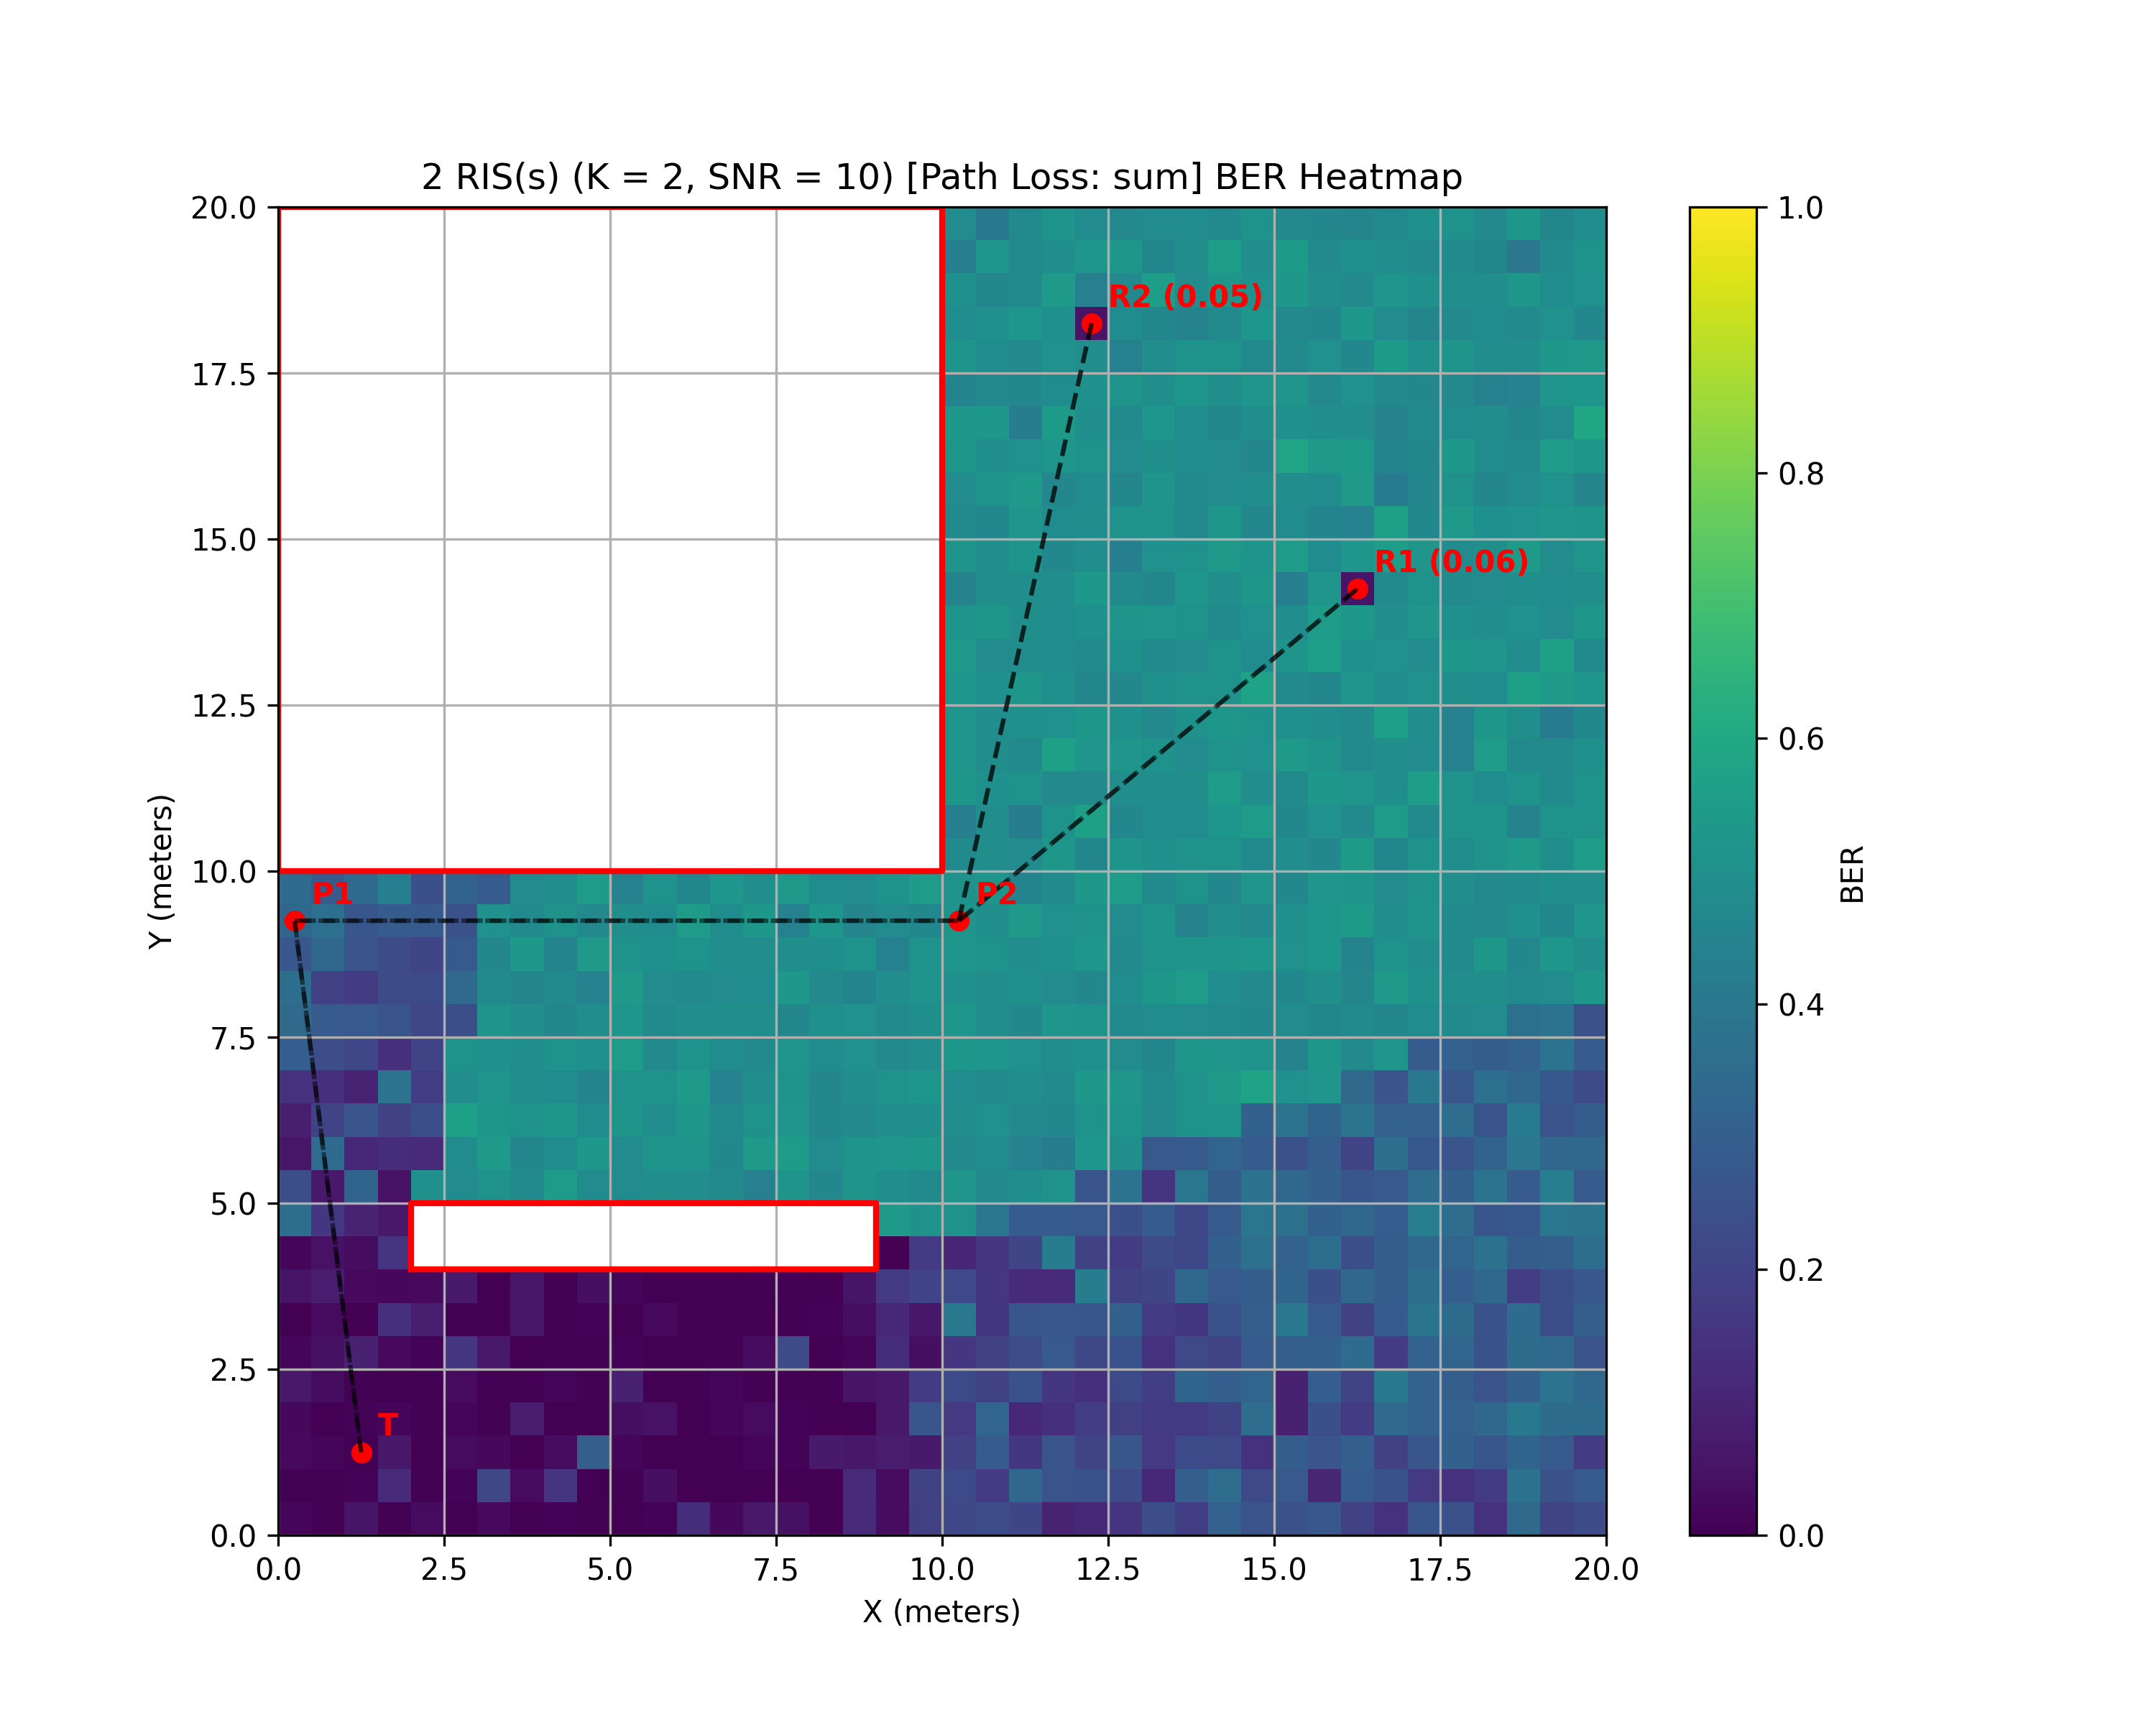
\includegraphics[width=\textwidth]{imgs/heatmap-simulations/2 RIS(s) (K = 2, SNR = 10) [Path Loss_ sum] BER Heatmap.png}
    \caption{BER Heatmap}
  \end{subfigure}
  \hfill
  \begin{subfigure}[b]{0.48\textwidth}
    \centering
    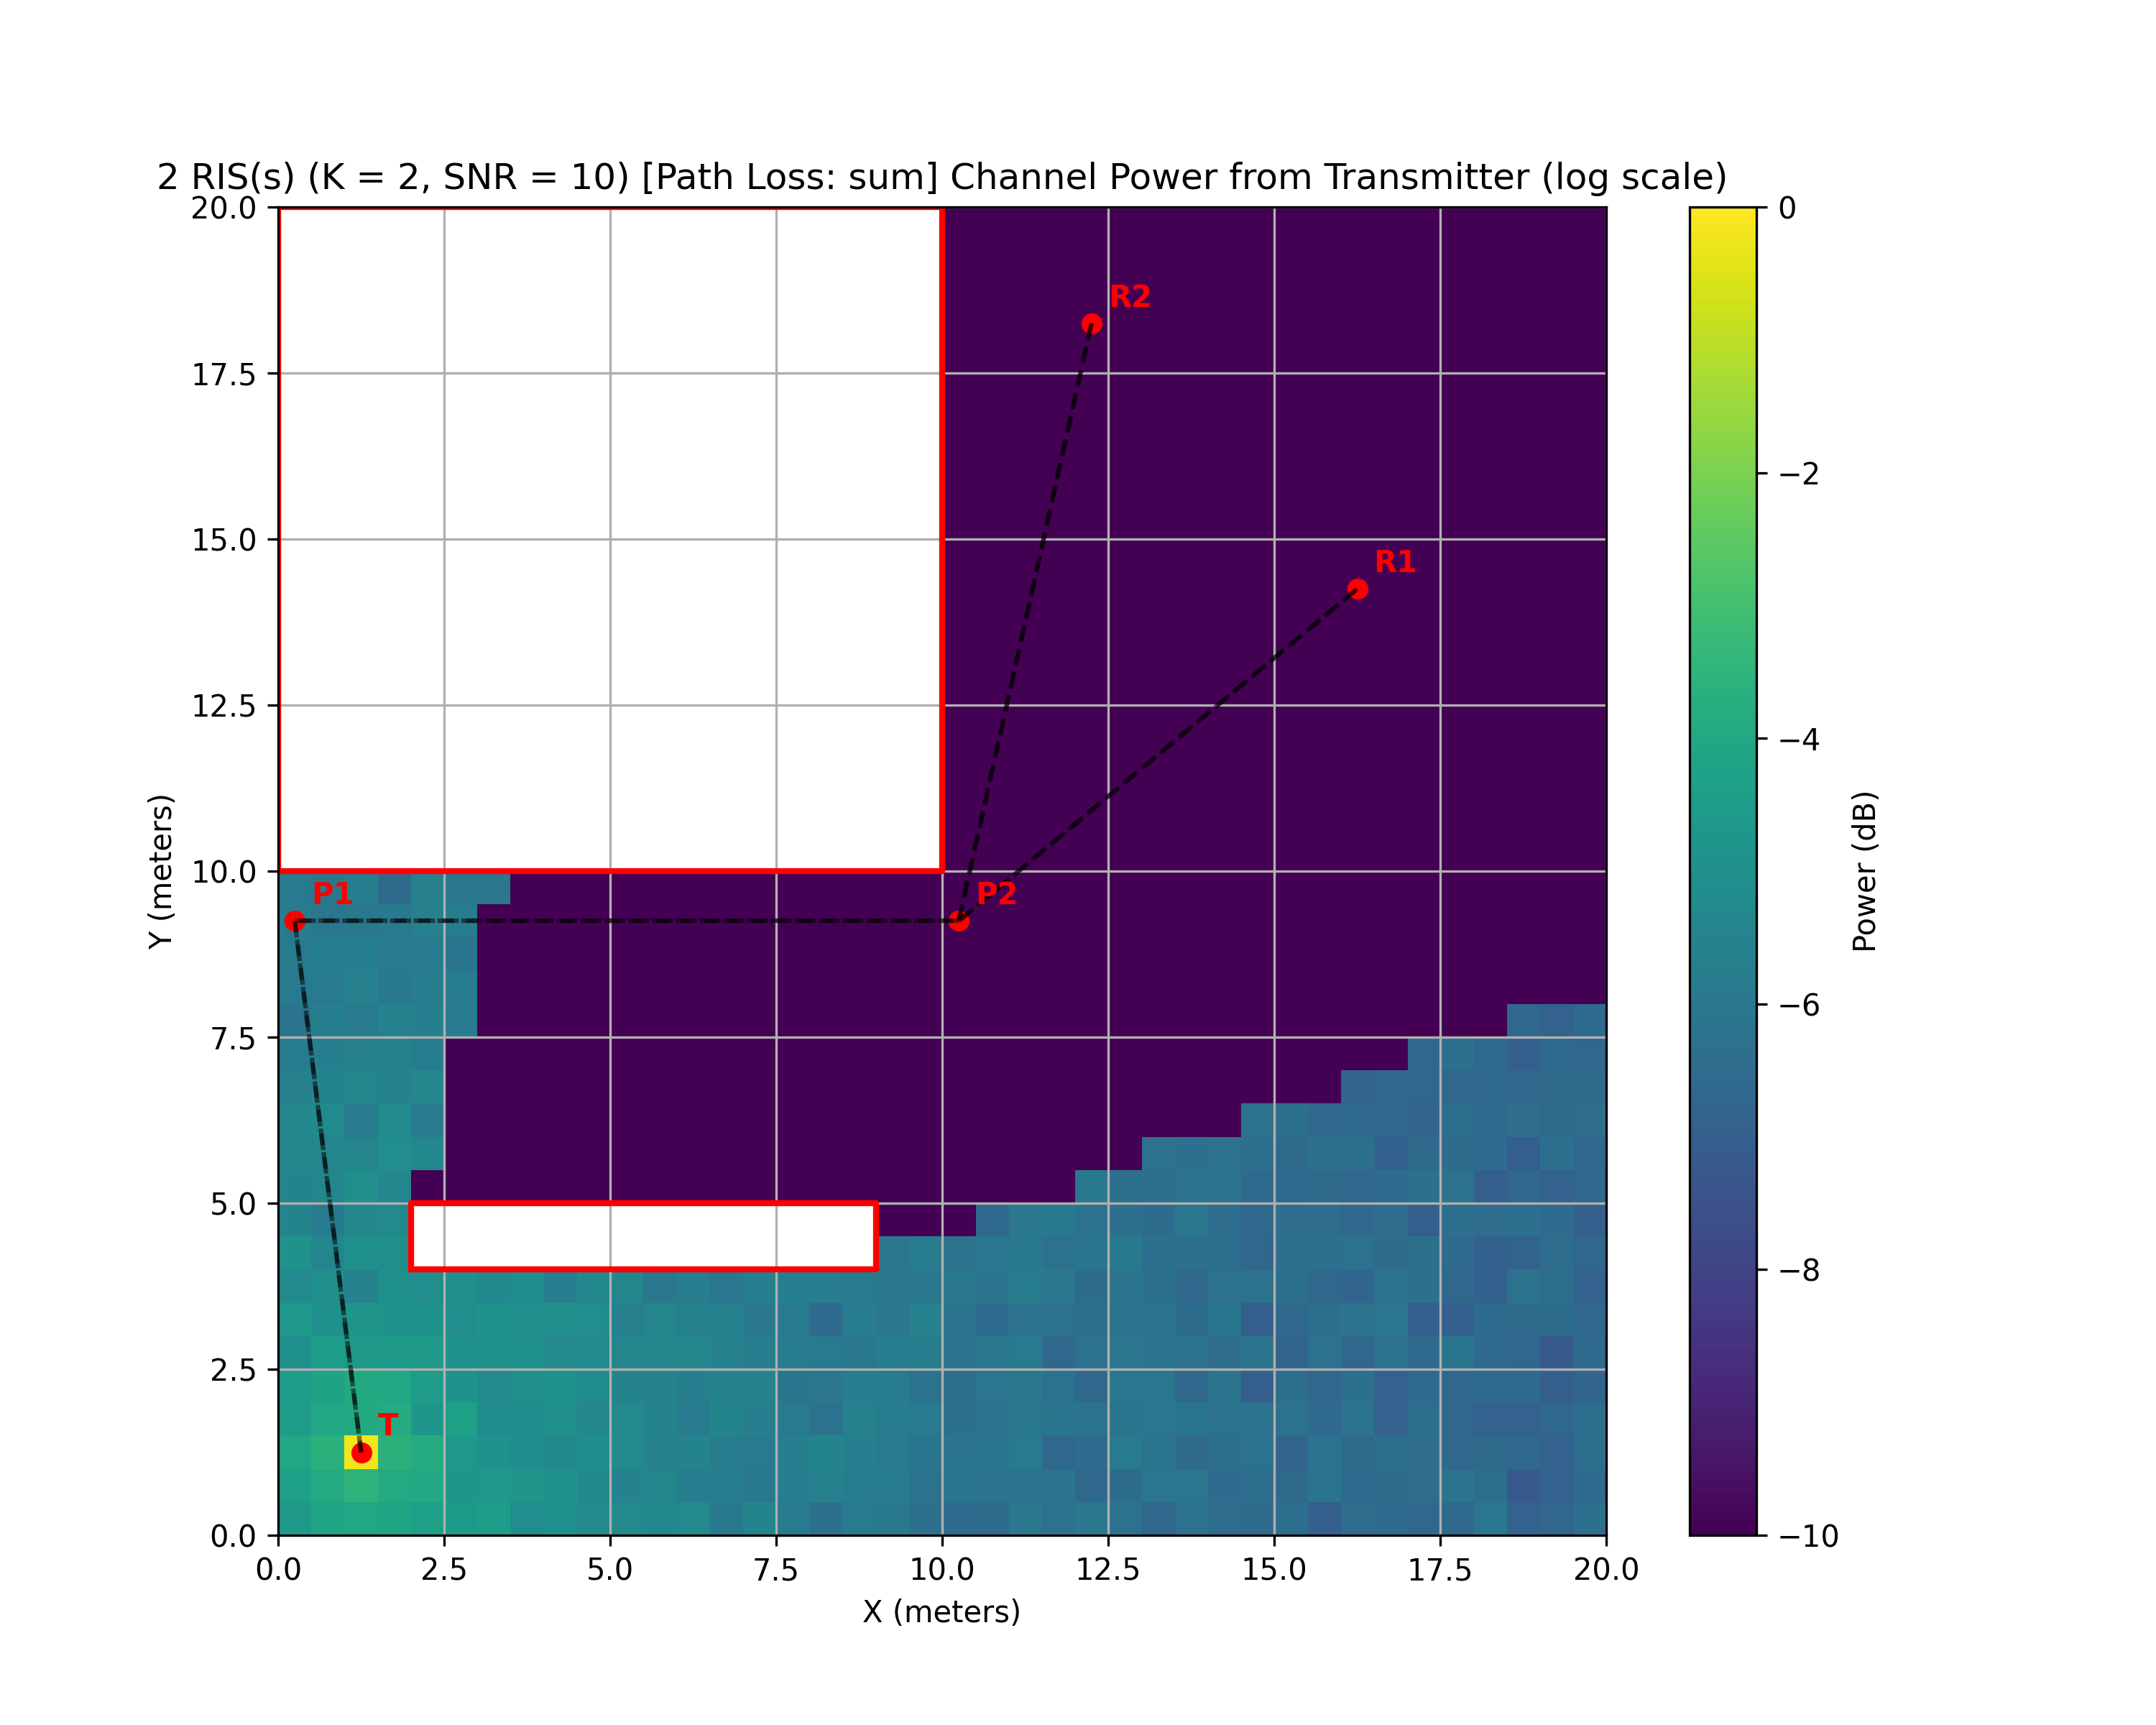
\includegraphics[width=\textwidth]{imgs/heatmap-simulations/2 RIS(s) (K = 2, SNR = 10) [Path Loss_ sum] Channel Power from Transmitter (log scale).png}
    \caption{Channel Power from Transmitter (log scale)}
  \end{subfigure}
  \medskip
  \centering
  \begin{subfigure}[b]{0.48\textwidth}
    \centering
    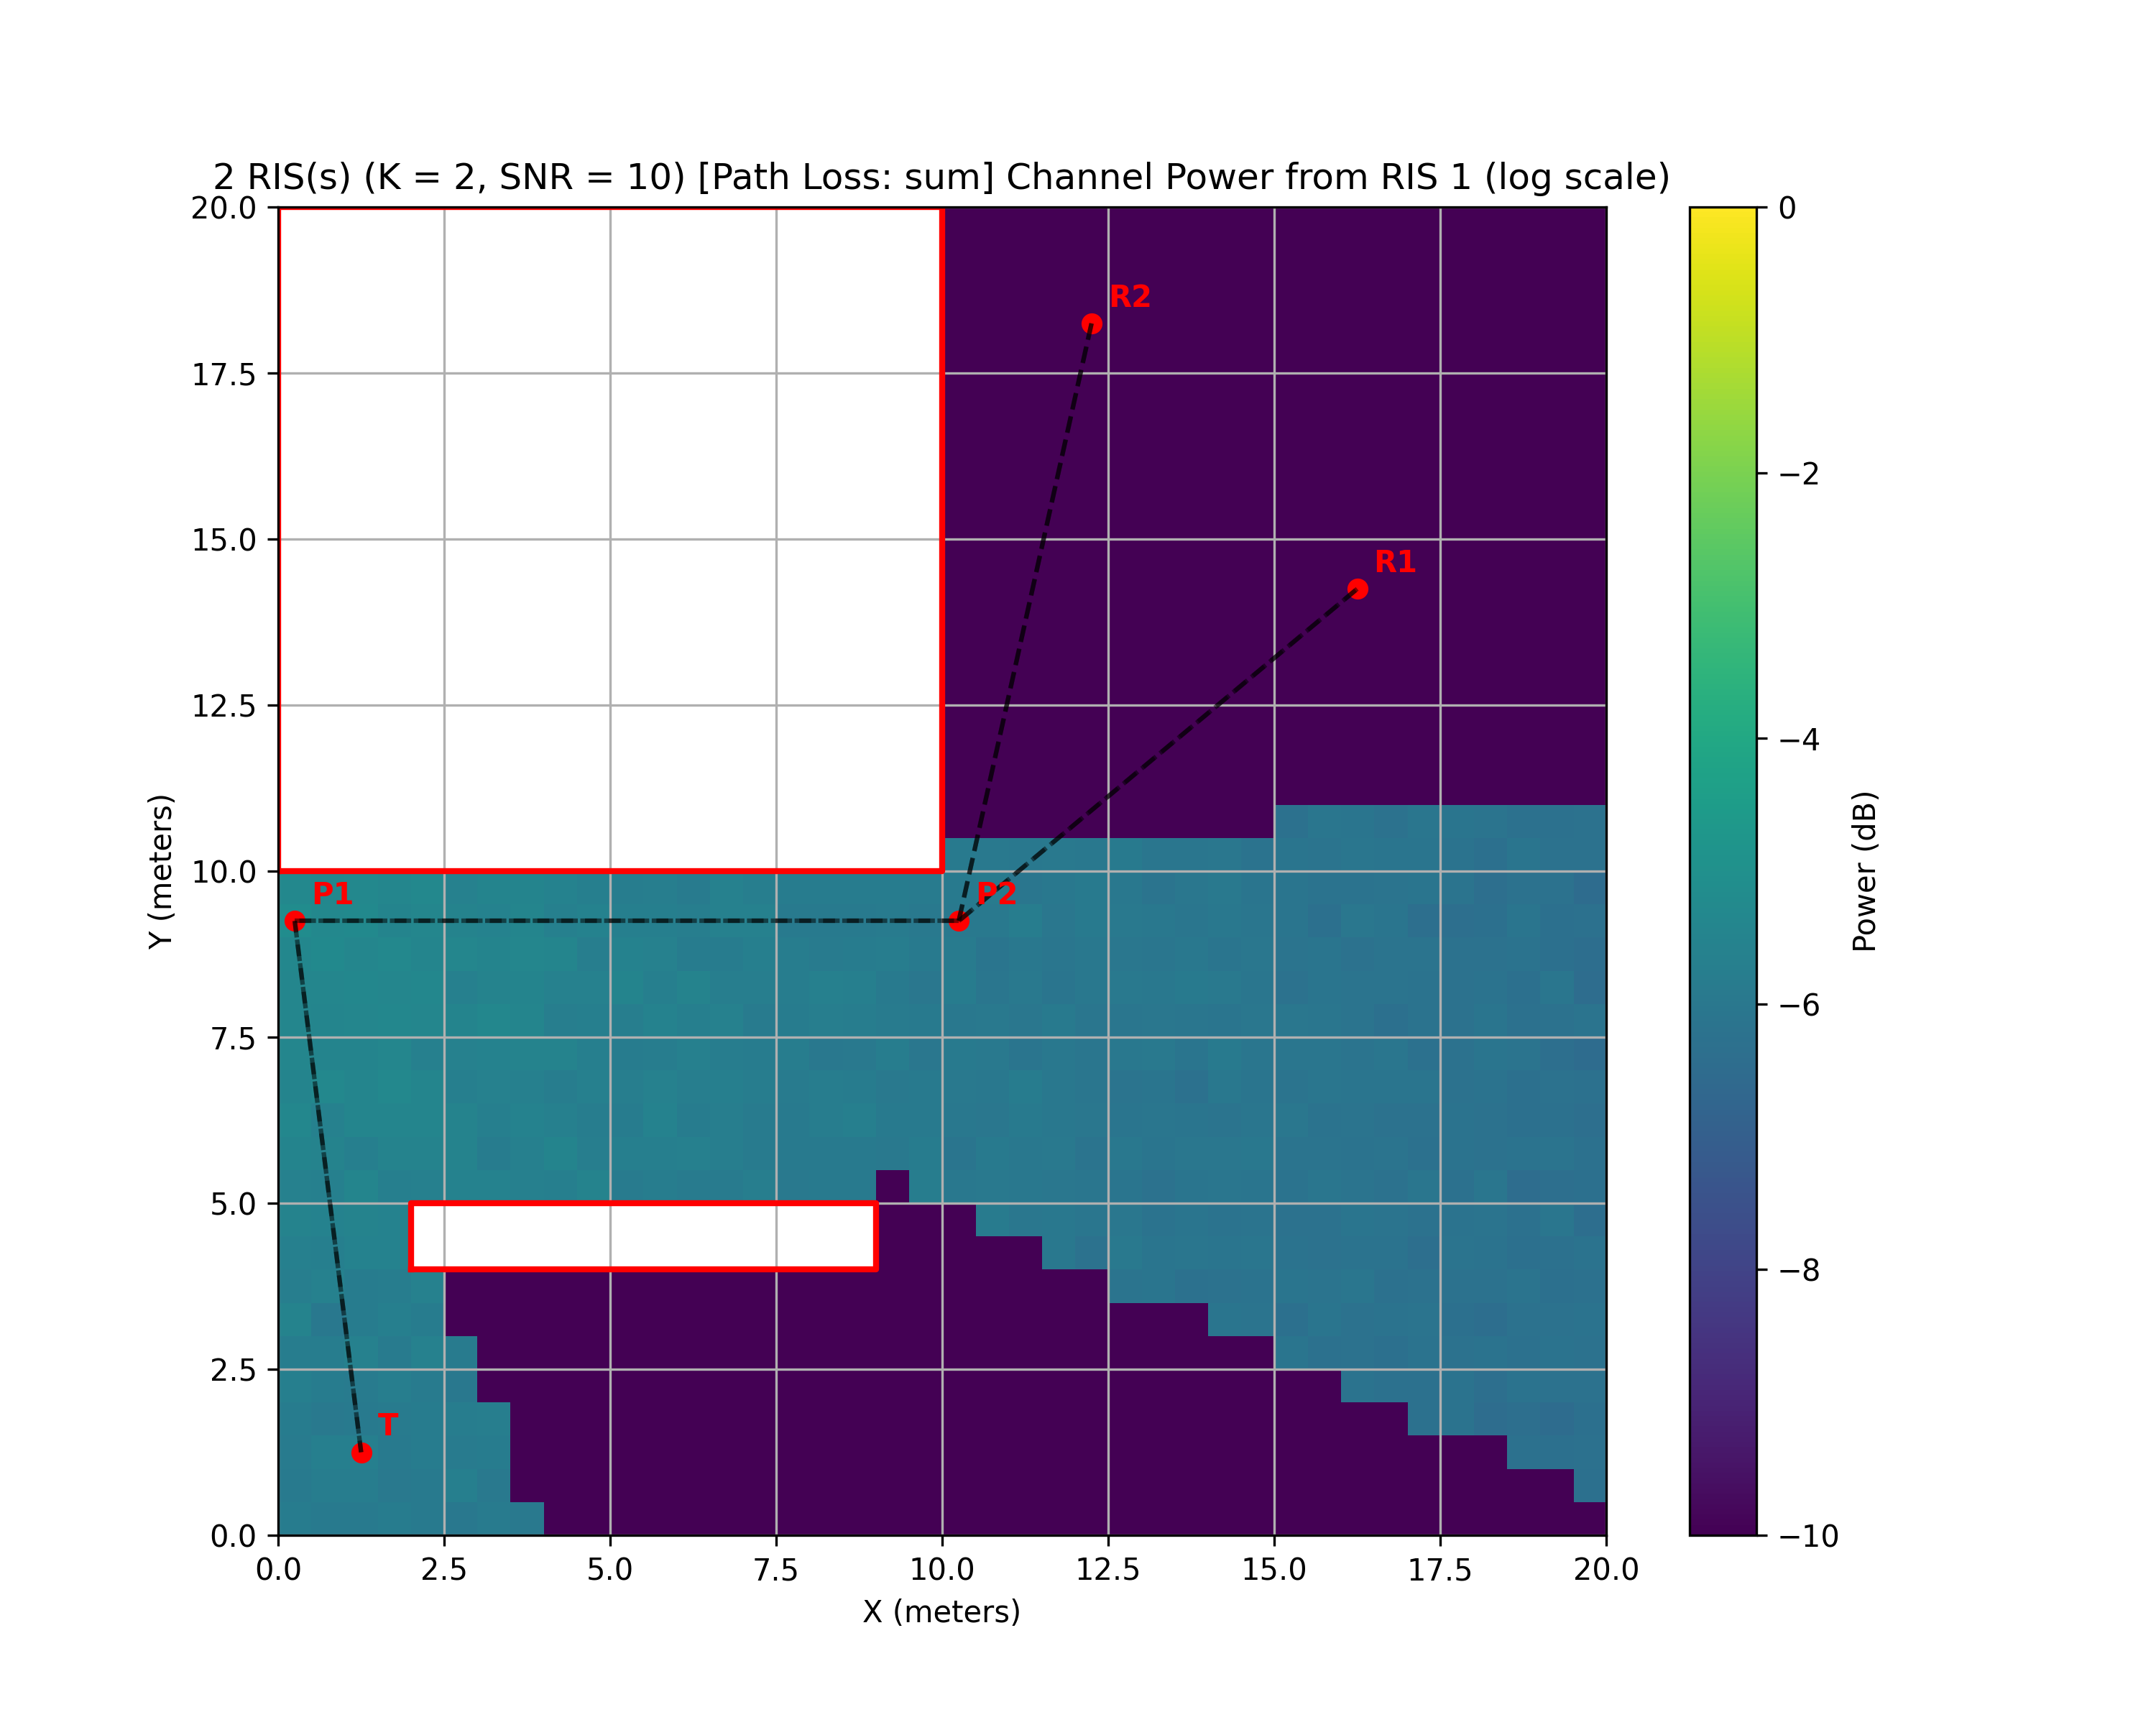
\includegraphics[width=\textwidth]{imgs/heatmap-simulations/2 RIS(s) (K = 2, SNR = 10) [Path Loss_ sum] Channel Power from RIS 1 (log scale).png}
    \caption{Channel Power from RIS 1 (log scale)}
  \end{subfigure}
  \hfill
  \begin{subfigure}[b]{0.48\textwidth}
    \centering
    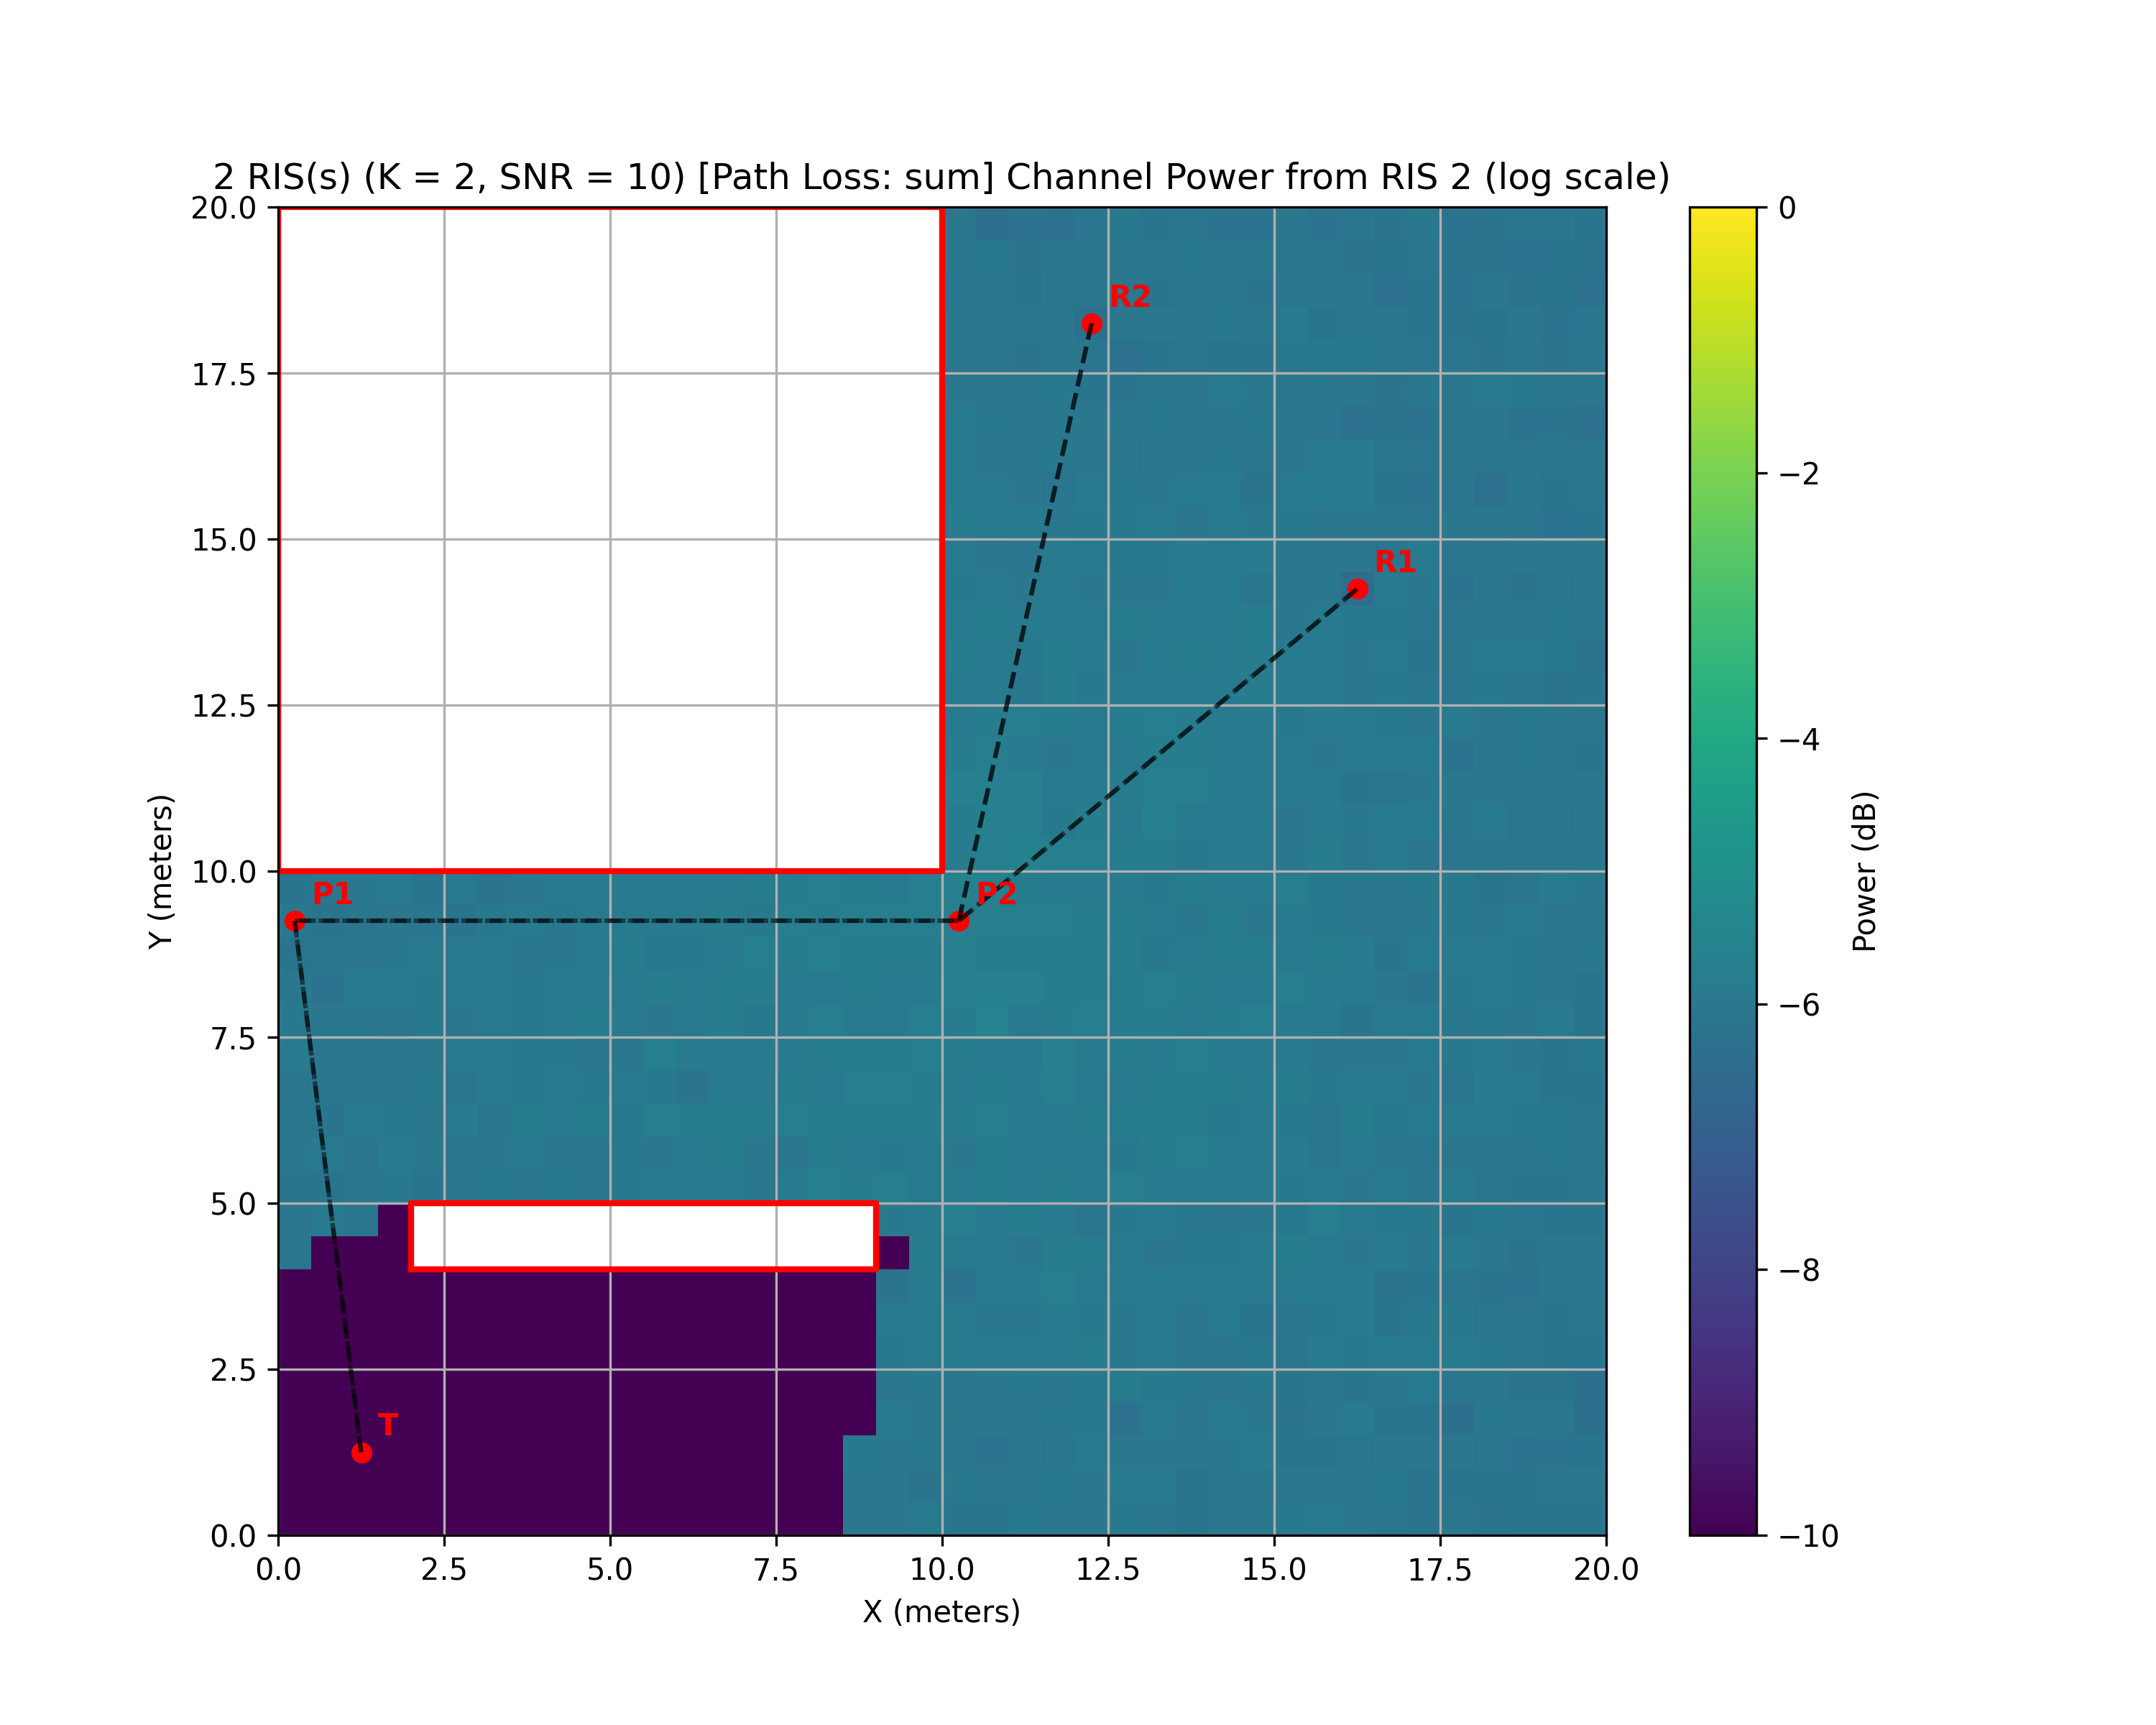
\includegraphics[width=\textwidth]{imgs/heatmap-simulations/2 RIS(s) (K = 2, SNR = 10) [Path Loss_ sum] Channel Power from RIS 2 (log scale).png}
    \caption{Channel Power from RIS 2 (log scale)}
  \end{subfigure}
  \caption{2 RIS(s) [Path Loss: sum]}
\end{figure}

\subsubsection{Heatmap conclusions}

We can see from the proposed path loss common properties:

\begin{itemize}
  \item with \textit{active path loss}, the RIS channel power is of the same order of magnitude as the transmitter channel power, so the direct signal receives significant noise. The problem is that, being an active RIS, it costs way more in both the deployment and the maintenance;
  \item with \textit{product path loss}, the RIS channel power is orders of magnitude smaller. The message remains hidden in areas without direct line of sight to the transmitter. If the budget is tight, or the direct LOS security is less needed compared to the NLOS security (for example, if the space in LOS with the transmitter is completely under control), this is an excellent possibility;
  \item with \textit{sum path loss}, the disturbance effect is still visible, although less effective. It also the one with the results most similar to the theoretical simulation we made in the previous section. Of course, the results must be considered keeping in mind that the RIS would be directional. It is an optimal choice for example to provide noise in a specific area, or if the scenario is composed of tight hallways.
\end{itemize}

Depending on the scenario, the budget and the level of security and obscuration needed, our framework provides an excellent choice for different kinds of situations and contexts.

Unfortunately, for specific vehicular applications, our framework is not really flexible due to the specific relation between the position, the distance and the channel gain matrix which then influence the readability of the signal. Our framework is still usable and highly recommended for static antennas and actors. For example, in a crossroad fixed antennas could communicate with the cars in the LOS using standard communication protocols, and with each other using RIS and our framework. The autonomous cars could also implement a traffic light - free crossroad queue system, when they would stop, communicate and coordinate with each other for who can go first. Common distributed algorithms for leader election could be used, like the \textit{Bully Algorithm} \cite{Bully_algorithm}.

It should be noted that the main difficulty in using our framework in conjunction with high speed moving vehicles is because of the channel gain estimation, since we do not only need the current one, but predict the next one where the car would go. Promising results are already coming in like in the paper "\textit{Adaptive Massive MIMO for fast moving connected vehicles: It will work with Predictor Antennas!}" \cite{8385489}, which studies how to use a different set of antennas, called Predictor Antennas, used to predict the main one channel gain with great accuracy. Similar literature can be found, showing a great interest in the field. For example, we also cite "\textit{Channel Estimation for Reconfigurable Intelligent Surface Assisted High-Mobility Wireless Systems}" \cite{9875062}, which proposes a new way to mitigate the error deriving from the movement speed, \textit{achieving substantial power efficiency improvements} at speeds up to 140 km/h and with as few as $N=16$ RIS elements.
\section{Conclusion}

In this paper, we have expanded on the work presented in \cite{9328149} regarding Physical Layer Security using Reconfigurable Intelligent Surfaces (RISs). We generalized the framework to support multiple receiving users and multiple RIS configurations, both in parallel and in series. By mathematically proving the formulas, and physically simulating realistic scenarios, we demonstrated the validity and usefulness of the prooposed work.

With our contribution, the framework is now able to manage:
\begin{itemize}
  \item Multiple receivers in different positions
  \item Multiple RISs in parallel that increase signal quality and security
  \item Multiple RISs working in series to accomodate complex situation
  \item A wide combination of these properties in realistic network conditions
\end{itemize}

With our Bit Error Rate (BER) simulations, we proved and demostrated how the receivers are able to receive correctly the messages with a low error percenteage, while ensuring no other malicious actor can decypher the signal when not having direct Line of Sight (LOS) from the transmitter. Even when this link is present, our configurations ensure the RIS distrupt the interception of the signal with significant noise, even at high Signal to Noise Ratio (SNR).

We also showed the realistic application of our framework in a simulated scenario including realistic channel gain calculations, adding Rician fading and considering signal strenght using path loss. These added simulation will aid exporting our solution from a mathematical proof to an effectivle implementation usable for real life communication. We modeled different possibilities of path loss and RIS implementation to cover all possible variables, showing promising results even in the worst scenarios.

The implications of this work are particularly relevant for emerging technologies such as vehicular networks, Internet of Things, and other applications requiring secure wireless communications. Thanks to modern technologies, we are able to increase the security and privacy even at lower layers of communication, helping reducing the load on higher layers wich could impact negatively the usefulness of communications when latency and frequency of communication is crucial.

\subsection{Future directions}

Future research directions could include:
\begin{itemize}
  \item Further optimization of RIS configurations for dynamic environments with mobile nodes
  \item Integration with existing security protocols at higher network layers
  \item Usage of more complex communication protocol, like GSSK \cite{4699782} instead of the proposed SSK \cite{5165332}
  \item Implementation and testing in real-world scenarios, particularly in vehicular networks
  \item Extension to even more complex network topologies with multiple transmitters and heterogeneous receiver capabilities
\end{itemize}

In particular, there is ample work that is possible to make in the heatmap simulations. For example, parallelization and the introduction of multiple RIS paths could be added, and a GUI to graphically setup the environment could be the start of a complex simulation environment.

The different type of path loss could be expanded in a more complete study of the different kind of RIS: what would be the mathematical differences in applying our framework for active and passive RIS, for uniform and directional ones? A simulation tool that could combine all these charateristics could be of great addition to the field of futuristic telecommunications.

Also, the entire field of Channel State Information (CSI), which here was introduced only in the part about Channel Gain matrix estimation, could also be simulated in our proposed tool and framework. Instead of using the physical calculated CSI, actors and RIS could try communicate using estimations of it and then verify the actual realistic results, including in our software estimation simulation functions.

The implementation of our research in vehicular networks is also an interesting topic directly linked to the CSI one. Expanding the context here with modern research on channel estimation of moving actors could transform our proposed work in a promising candidate for the future of autonomous telecommunications.

In conclusion, our extended framework for physical layer security using RISs provides a promising approach to secure modern wireless communication systems, especially in scenarios where traditional encryption methods may introduce unacceptable computational overhead or latency. The flexibility to support multiple users and complex reflection paths makes it adaptable to various practical deployment scenarios while maintaining strong security guarantees.



\endgroup


% bibliography - bibtex format
%
% add chapter to index
\addcontentsline{toc}{chapter}{Bibliography}
% alphabetical order of authors
\bibliographystyle{plain}
\bibliography{references}
%%%%%%%%%%%%%%%%%%%%%%%%%%%%%%%%%%%%%%%%%%%%%%%%%%%%%%%%%%%%%%%%%%%%%%%%%%
%%%%%%%%%%%%%%%%%%%%%%%%%%%%%%%%%%%%%%%%%%%%%%%%%%%%%%%%%%%%%%%%%%%%%%%%%%
%% Nota
%%%%%%%%%%%%%%%%%%%%%%%%%%%%%%%%%%%%%%%%%%%%%%%%%%%%%%%%%%%%%%%%%%%%%%%%%%
%% In the bibliography, all the sources consulted for the dissertation 
%% have to be cited and listed in alphabetical order by the 
%% first author's surname.
%%
%% According to the source material, the quotation has to be as follows:
%%
%% BOOKS
%% Surname and initial/s of the name/s of the author/s, date of edition,
%% publishing house and (if applicable) number of edition.
%% 
%% JOURNAL ARTICLES 
%% Surname and initial/s of the first name/s of the author/s,
%% title of the article, name of the journal, volume number, issue number
%% and page numbers.
%% 
%% CONFERENCE PAPERS
%% Surname and initial/s of the name/s of the author/s,
%% year of the conference, title of the article, name of the conference,
%% place of the conference, conference dates, page numbers.
%% 
%% CITING WEB RESOURCES
%% The consulted webpages have to be listed in alphabetical order. 
%% It is necessary to:
%%   - Copy the specific URL (the web address) of the consulted webpage
%%   - If available, indicate the surname and first name of the author/s,
%%     the title and subtitle of the text
%%   - If available, indicate the last date you retrieved the webpage
%%     (day/month/year).   
%%%%%%%%%%%%%%%%%%%%%%%%%%%%%%%%%%%%%%%%%%%%%%%%%%%%%%%%%%%%%%%%%%%%%%%%%%
%%%%%%%%%%%%%%%%%%%%%%%%%%%%%%%%%%%%%%%%%%%%%%%%%%%%%%%%%%%%%%%%%%%%%%%%%%


\titleformat{\chapter}
{\normalfont\Huge\bfseries}{Appendix \thechapter}{1em}{}
% % Appendix / attachment section - optional
\appendix
% \chapter{Title first appendix}

Lorem ipsum dolor sit amet, consectetur adipiscing elit. Donec sed nunc orci. Aliquam nec nisl vitae sapien pulvinar dictum quis non urna. Suspendisse at dui a erat aliquam vestibulum. Quisque ultrices pellentesque pellentesque. Pellentesque egestas quam sed blandit tempus. Sed congue nec risus posuere euismod. Maecenas ut lacus id mauris sagittis egestas a eu dui. Class aptent taciti sociosqu ad litora torquent per conubia nostra, per inceptos himenaeos. Pellentesque at ultrices tellus. Ut eu purus eget sem iaculis ultricies sed non lorem. Curabitur gravida dui eget ex vestibulum venenatis. Phasellus gravida tellus velit, non eleifend justo lobortis eget. 

\section{Title}
Lorem ipsum dolor sit amet, consectetur adipiscing elit. Donec sed nunc orci. Aliquam nec nisl vitae sapien pulvinar dictum quis non urna. Suspendisse at dui a erat aliquam vestibulum. Quisque ultrices pellentesque pellentesque. Pellentesque egestas quam sed blandit tempus. Sed congue nec risus posuere euismod. Maecenas ut lacus id mauris sagittis egestas a eu dui. Class aptent taciti sociosqu ad litora torquent per conubia nostra, per inceptos himenaeos. Pellentesque at ultrices tellus. Ut eu purus eget sem iaculis ultricies sed non lorem. Curabitur gravida dui eget ex vestibulum venenatis. Phasellus gravida tellus velit, non eleifend justo lobortis eget. 

\subsection{Sub-title}
Lorem ipsum dolor sit amet, consectetur adipiscing elit. Donec sed nunc orci. Aliquam nec nisl vitae sapien pulvinar dictum quis non urna. Suspendisse at dui a erat aliquam vestibulum. Quisque ultrices pellentesque pellentesque. Pellentesque egestas quam sed blandit tempus. Sed congue nec risus posuere euismod. Maecenas ut lacus id mauris sagittis egestas a eu dui. Class aptent taciti sociosqu ad litora torquent per conubia nostra, per inceptos himenaeos. Pellentesque at ultrices tellus. Ut eu purus eget sem iaculis ultricies sed non lorem. Curabitur gravida dui eget ex vestibulum venenatis. Phasellus gravida tellus velit, non eleifend justo lobortis eget. 


\chapter{Title first appendix}

Lorem ipsum dolor sit amet, consectetur adipiscing elit. Donec sed nunc orci. Aliquam nec nisl vitae sapien pulvinar dictum quis non urna. Suspendisse at dui a erat aliquam vestibulum. Quisque ultrices pellentesque pellentesque. Pellentesque egestas quam sed blandit tempus. Sed congue nec risus posuere euismod. Maecenas ut lacus id mauris sagittis egestas a eu dui. Class aptent taciti sociosqu ad litora torquent per conubia nostra, per inceptos himenaeos. Pellentesque at ultrices tellus. Ut eu purus eget sem iaculis ultricies sed non lorem. Curabitur gravida dui eget ex vestibulum venenatis. Phasellus gravida tellus velit, non eleifend justo lobortis eget. 

\section{Title}
Lorem ipsum dolor sit amet, consectetur adipiscing elit. Donec sed nunc orci. Aliquam nec nisl vitae sapien pulvinar dictum quis non urna. Suspendisse at dui a erat aliquam vestibulum. Quisque ultrices pellentesque pellentesque. Pellentesque egestas quam sed blandit tempus. Sed congue nec risus posuere euismod. Maecenas ut lacus id mauris sagittis egestas a eu dui. Class aptent taciti sociosqu ad litora torquent per conubia nostra, per inceptos himenaeos. Pellentesque at ultrices tellus. Ut eu purus eget sem iaculis ultricies sed non lorem. Curabitur gravida dui eget ex vestibulum venenatis. Phasellus gravida tellus velit, non eleifend justo lobortis eget. 

\subsection{Sub-title}
Lorem ipsum dolor sit amet, consectetur adipiscing elit. Donec sed nunc orci. Aliquam nec nisl vitae sapien pulvinar dictum quis non urna. Suspendisse at dui a erat aliquam vestibulum. Quisque ultrices pellentesque pellentesque. Pellentesque egestas quam sed blandit tempus. Sed congue nec risus posuere euismod. Maecenas ut lacus id mauris sagittis egestas a eu dui. Class aptent taciti sociosqu ad litora torquent per conubia nostra, per inceptos himenaeos. Pellentesque at ultrices tellus. Ut eu purus eget sem iaculis ultricies sed non lorem. Curabitur gravida dui eget ex vestibulum venenatis. Phasellus gravida tellus velit, non eleifend justo lobortis eget. 



\section{Code Implementation}

To validate our theoretical framework, we have implemented a simulation environment in Python that allows us to test both our mathematical models and their real-world applicability. The codebase consists of three main modules: diagonalization, bit error rate (BER) analysis, and a heatmap generator to visualize the spatial distribution of signal quality.

\subsection{Diagonalization Module}

The diagonalization module implements the core mathematical concepts of our RIS reflection framework, following the theoretical foundation presented in Section 3 and 4.

\subsubsection{Null Space Calculation}
We first start by making the calculation of reflection matrices, which ensure the effective channel between the transmitter and receiver is diagonalized. We implement this through the \texttt{calculate\_W\_single} and \texttt{calculate\_W\_multiple} functions:

\begin{lstlisting}[language=python, caption={Calculation of W matrices}]
def calculate_W_single(K: int, N: int, G: np.ndarray, H: np.ndarray) -> np.ndarray:
    """
    Calculate W matrix for a single receiver.
    
    Args:
        K: Number of antennas
        N: Number of reflecting elements
        G: Channel matrix from RIS to receiver (KxN)
        H: Channel matrix from transmitter to RIS (NxK)
    
    Returns:
        W: The W matrix as defined in equation (8) of the paper
    """
    W = np.zeros((N, N), dtype=complex)
    
    for i in range(K):
        for j in range(K):
            if i != j:
                temp = np.multiply(G[j, :], H[:, i].T)
                W += np.outer(temp.conj(), temp)
    
    return W
\end{lstlisting}

This function calculates the W matrix for a single receiver. For multiple receivers, we stack these matrices:

\begin{lstlisting}[language=python, caption={W matrix for multiple receivers}]
def calculate_W_multiple(K: int, N: int, J: int, Gs: List[np.ndarray], H: np.ndarray) -> np.ndarray:
    """
    Calculate combined W matrix for multiple receivers.
    """
    W_combined = np.zeros((J * N, N), dtype=complex)
    
    for j in range(J):
        W_j = calculate_W_single(K, N, Gs[j], H)
        W_combined[j*N:(j+1)*N, :] = W_j
    
    return W_combined
\end{lstlisting}

\subsubsection{RIS Reflection Matrix Calculation}

With the W matrix defined, we can calculate the reflection matrices using Singular Value Decomposition (SVD) to find the null space:

\begin{lstlisting}[language=python, caption={RIS Reflection Matrix Calculation}]
def calculate_ris_reflection_matrice(
    K: int, 
    N: int, 
    J: int, 
    Gs: List[np.ndarray], 
    H: np.ndarray, 
    eta: float,
) -> Tuple[np.ndarray, float]:
    """
    Calculate reflection matrices for RIS surfaces.
    """
    W = calculate_W_multiple(K, N, J, Gs, H)
    U, sigma, Vh = np.linalg.svd(W)
    
    null_space_dim = N - J*K**2 + J*K
    if null_space_dim <= 0:
        raise ValueError(f"No solution exists. Need more reflecting elements.")
    
    first_singular_values = sigma[:N - null_space_dim]
    last_singular_values = sigma[-null_space_dim:]
    
    null_space_basis = Vh[-null_space_dim:, :].T.conj()

    if null_space_basis.shape != (N, null_space_dim):
        raise ValueError(f"Invalid null space basis shape.")

    a = np.random.normal(0, 1, (null_space_dim,)) + 1j * np.random.normal(0, 1, (null_space_dim,))
    
    p_unnormalized = null_space_basis @ a
    p = eta * p_unnormalized / np.max(np.abs(p_unnormalized))
    P = np.diag(p)
    dor = 2 * null_space_dim
    return P, dor
\end{lstlisting}

This function implements the theoretical approach described in Section 4.1, where we find the null space of W and then generate a random vector in this space to ensure randomness in our reflection coefficients.

\subsubsection{Multiple RIS Support}

To support multiple RIS surfaces in series, we implemented:

\begin{lstlisting}[language=python, caption={Multiple RIS calculation}]
def calculate_multi_ris_reflection_matrices(
    K: int, 
    N: int, 
    J: int, 
    M: int,
    Gs: List[np.ndarray], 
    H: np.ndarray, 
    eta: float,
    Cs: List[np.ndarray]
) -> Tuple[List[np.ndarray], float]:
    """
    Calculate reflection matrices for M RIS surfaces.
    """
    if len(Cs) != M-1:
        raise ValueError(f"Expected {M-1} inter-RIS channel matrices.")

    ps = []
    S = np.eye(N)

    # Generate M-1 random reflection vectors
    for i in range(M-1):
        absorptions = np.random.uniform(0, 1, N)
        phases = np.random.uniform(0, 2*np.pi, N)
        # p_m[i] = eta * r_i * exp(j*theta_i)
        p_m = absorptions * np.exp(1j * phases)
        ps.append(p_m)
        S = S @ np.diag(p_m) @ Cs[i]

    Gs_prime = [G @ S for G in Gs]
    
    # Calculate the last reflection matrix
    P_final, dor = calculate_ris_reflection_matrice(K, N, J, Gs_prime, H, eta)
    p_final = np.diag(P_final)
    ps.append(p_final)

    Ps = []
    for pm in ps:
        Ps.append(np.diag(pm))
    
    return Ps, dor
\end{lstlisting}

This implements our approach from Section 4.3, where we generate random reflection coefficients for all but the last RIS, then calculate the last one to ensure diagonalization.

\subsubsection{Unified Reflection Matrix}

For convenience in calculations, we provide a function to unify multiple reflection matrices into a single effective matrix:

\begin{lstlisting}[language=python, caption={Unifying RIS matrices}]
def unify_ris_reflection_matrices(Ps: List[np.ndarray], Cs: List[np.ndarray]) -> np.ndarray:
    """
    Unify reflection matrices into a single matrix.
    """
    P = Ps[0]
    for i in range(len(Ps)-1):
        P = P @ Cs[i] @ Ps[i+1]
    return P
\end{lstlisting}

\subsubsection{Verification}

We also implement verification functions to ensure our theoretical expectations match the implementation:

\begin{lstlisting}[language=python, caption={Verification of diagonalization}]
def verify_multi_ris_diagonalization(
    Ps: List[np.ndarray],
    Gs: List[np.ndarray],
    H: np.ndarray,
    Cs: List[np.ndarray]
) -> List[bool]:
    """
    Verify that G(P_1C_1P_2C_2...P_M)H is diagonal for all receivers.
    """
    results = []
    
    P = unify_ris_reflection_matrices(Ps, Cs)
    for G in Gs:
        effective_channel = G @ P @ H
        off_diag_sum = np.sum(np.abs(effective_channel - np.diag(np.diag(effective_channel))))
        results.append(off_diag_sum < tolerance)
    return results
\end{lstlisting}

\subsection{BER Module}

The BER (Bit Error Rate) module implements the simulation of space shift keying (SSK) transmissions and calculates the error rates under different scenarios.

\subsubsection{SSK Transmission Simulation}

We simulate SSK transmission with the following core functions:

\begin{lstlisting}[language=python, caption={SSK Transmission Simulation}]
def simulate_ssk_transmission(K: int, sigma_sq: float, calculate_detected_id: Callable[[np.ndarray, np.ndarray], float]):
    n_bits = int(np.log2(K))
    if 2**n_bits != K:
        raise ValueError(f"K must be a power of 2, got {K}")
    bit_mappings = np.array([format(i, f'0{n_bits}b') for i in range(K)])    
    true_bits = np.random.randint(0, 2, n_bits)
    true_bits_str = ''.join(map(str, true_bits))
    true_idx = np.where(bit_mappings == true_bits_str)[0][0]

    x = np.zeros(K)
    x[true_idx] = 1

    noise = create_random_noise_vector(K, sigma_sq)
    detected_idx = calculate_detected_id(x, noise)
    
    detected_bits = np.array(list(bit_mappings[detected_idx])).astype(int)
    errors = np.sum(detected_bits != true_bits)
    return errors / n_bits
\end{lstlisting}

This function implements the common core of our SSK transmission simulation. It maps bits to antenna indices, simulates transmission with noise, and calculates the error rate.

We then implement specialized versions for reflection and direct transmission:

\begin{lstlisting}[language=python, caption={SSK Transmission with Reflection}]
def simulate_ssk_transmission_reflection(K: int, effective_channel: np.ndarray, sigma_sq: float):
    if effective_channel.shape != (K, K):
        raise ValueError(f"Reflection: Effective channel shape must be ({K}, {K})")

    def calculate_detected_id(x: np.ndarray, noise: np.ndarray):
        y = effective_channel @ x + noise
        return np.argmax(np.abs(y)**2)
    
    return simulate_ssk_transmission(K, sigma_sq, calculate_detected_id)
\end{lstlisting}

\begin{lstlisting}[language=python, caption={SSK Transmission with Direct Path}]
def simulate_ssk_transmission_direct(K: int, B: np.ndarray, effective_channel: np.ndarray, sigma_sq: float):
    if B.shape != (K, K):
        raise ValueError(f"Direct: B shape must be ({K}, {K})")
    
    if effective_channel.shape != (K, K):
        raise ValueError(f"Direct: Effective channel shape must be ({K}, {K})")

    def calculate_detected_id(x: np.ndarray, noise: np.ndarray):
        y = (B + effective_channel) @ x + noise
        distances = np.array([np.linalg.norm(y - B[:, i]) for i in range(B.shape[1])])
        return np.argmin(distances)
    
    return simulate_ssk_transmission(K, sigma_sq, calculate_detected_id)
\end{lstlisting}

These functions implement the detection methods described in Section 3.2, where the legitimate receiver can detect the signal through the diagonalized channel, while the eavesdropper hears from the direct path and receives interference from the reflection.

\subsubsection{BER Simulation}

We also implement a comprehensive BER simulation function that evaluates performance across different SNR values:

\begin{lstlisting}[language=python, caption={BER Simulation}]
def calculate_ber_simulation(snr_db, K, N, J, M, eta=0.9, num_symbols=10000):
    sigma_sq = snr_db_to_sigma_sq(snr_db)
    errors_receiver = 0
    errors_eavesdropper = 0
    errors_direct = 0
    
    errors_receiver_double = 0
    errors_eavesdropper_double = 0
    
    for _ in range(num_symbols):
        # Generate channel matrices
        H = generate_random_channel_matrix(N, K)
        Gs = [generate_random_channel_matrix(K, N) for _ in range(J)]
        G = random.choice(Gs)
        Fs = [generate_random_channel_matrix(K, N) for _ in range(M)]
        B = generate_random_channel_matrix(K, K)
        Cs = [generate_random_channel_matrix(N, N) for _ in range(M-1)]
        
        # Calculate reflection matrices
        Ps, _ = calculate_multi_ris_reflection_matrices(K, N, J, M, Gs, H, eta, Cs)
        P = unify_ris_reflection_matrices(Ps, Cs)

        # Calculate effective channels
        effective_channel_receiver = G @ P @ H
        effective_channel_eavesdropper = np.zeros((K, K), dtype=np.complex128)
        for i in range(M):
            P_to_i = unify_ris_reflection_matrices(Ps[:i+1], Cs[:i])
            effective_channel_eavesdropper += Fs[i] @ P_to_i @ H
        effective_channel_direct = np.zeros((K, K))

        # Simulate transmissions
        errors_receiver += simulate_ssk_transmission_reflection(K, effective_channel_receiver, sigma_sq)
        errors_eavesdropper += simulate_ssk_transmission_direct(K, B, effective_channel_eavesdropper, sigma_sq)
        errors_direct += simulate_ssk_transmission_direct(K, B, effective_channel_direct, sigma_sq)
        
        H2 = generate_random_channel_matrix(N, K)
        Gs2 = [generate_random_channel_matrix(K, N) for _ in range(J)]
        G2 = random.choice(Gs2)
        Fs2 = [generate_random_channel_matrix(K, N) for _ in range(M)]
        Cs2 = [generate_random_channel_matrix(N, N) for _ in range(M-1)]
        Ps2, _ = calculate_multi_ris_reflection_matrices(
            K, N, J, M, Gs2, H2, eta, Cs2
        )
        P2 = unify_ris_reflection_matrices(Ps2, Cs2)

        effective_channel_receiver_2 = G2 @ P2 @ H2
        effective_channel_eavesdropper_2 = np.zeros((K, K), dtype=np.complex128) # F @ P @ H
        for i in range(M):
            P_to_i = unify_ris_reflection_matrices(Ps2[:i+1], Cs2[:i])
            effective_channel_eavesdropper_2 += Fs2[i] @ P_to_i @ H2

        effective_channel_receiver_double = effective_channel_receiver + effective_channel_receiver_2
        effective_channel_eavesdropper_double = effective_channel_eavesdropper + effective_channel_eavesdropper_2

        errors_receiver_double += simulate_ssk_transmission_reflection(K, effective_channel_receiver_double, sigma_sq)
        errors_eavesdropper_double += simulate_ssk_transmission_direct(K, B, effective_channel_eavesdropper_double, sigma_sq)
    
    result_receiver = errors_receiver / num_symbols
    result_eavesdropper = errors_eavesdropper / num_symbols
    result_direct = errors_direct / num_symbols
    result_receiver_double = errors_receiver_double / num_symbols
    result_eavesdropper_double = errors_eavesdropper_double / num_symbols

    return result_receiver, result_eavesdropper, result_direct, result_receiver_double, result_eavesdropper_double
\end{lstlisting}

This function simulates BER performance across legitimate receivers and eavesdroppers, including scenarios with multiple RIS surfaces and different path configurations.

\subsection{Heatmap Generator}

To visualize our results in a spatial context, we implemented a heatmap generator that simulates signal quality across a 2D space:

\subsubsection{Core Heatmap Class}

\begin{lstlisting}[language=python, caption={Heatmap Generator Class}]
class HeatmapGenerator:
    def __init__(self, width: int, height: int, resolution: float = 0.5):
        """
        Initialize the heatmap generator with given dimensions.
        """
        self.width = width
        self.height = height
        self.resolution = resolution
        
        # Calculate grid dimensions based on resolution
        self.grid_width = int(width / resolution)
        self.grid_height = int(height / resolution)
        self.grid = np.zeros((self.grid_height, self.grid_width))
        self.buildings = []
        # Dictionary to store points with their labels and coordinates
        self.points = {}
\end{lstlisting}

The heatmap generator creates a grid-based representation of a physical space, where we can place transmitters, receivers, and obstacles.

\subsubsection{Building and Point Management}

\begin{lstlisting}[language=python, caption={Buildings and Points in Heatmap}]
def add_building(self, x: int, y: int, width: int, height: int):
    """
    Add a building to the map. Buildings are excluded from the heatmap calculation.
    """
    self.buildings.append((x, y, width, height))
    grid_x, grid_y = self._meters_to_grid(x, y)
    grid_width = int(width / self.resolution)
    grid_height = int(height / self.resolution)
    
    # Mark building area as NaN to exclude from heatmap
    self.grid[grid_y:grid_y+grid_height, grid_x:grid_x+grid_width] = np.nan

def add_point(self, label: str, x: float, y: float):
    """
    Add a point of interest to the map with a specific label.
    """
    if not (0 <= x < self.width and 0 <= y < self.height):
        raise ValueError(f"Point {label} coordinates ({x}, {y}) are outside the map boundaries")
    self.points[label] = (x, y)
\end{lstlisting}

These functions allow us to define the simulation environment with buildings (which block signals) and points representing transmitters, RIS surfaces, and receivers.

\subsubsection{Line of Sight Checking}

An important aspect of our simulation is determining whether two points have line-of-sight:

\begin{lstlisting}[language=python, caption={Line of Sight Checking}]
def _line_intersects_building(self, x1: float, y1: float, x2: float, y2: float) -> bool:
    """
    Check if line between two points intersects any building.
    Uses line segment intersection algorithm.
    """
    def ccw(A: tuple, B: tuple, C: tuple) -> bool:
        """Returns True if points are counter-clockwise oriented"""
        return (C[1] - A[1]) * (B[0] - A[0]) > (B[1] - A[1]) * (C[0] - A[0])

    def intersect(A: tuple, B: tuple, C: tuple, D: tuple) -> bool:
        """Returns True if line segments AB and CD intersect"""
        return ccw(A, C, D) != ccw(B, C, D) and ccw(A, B, C) != ccw(A, B, D)

    for bx, by, bw, bh in self.buildings:
        building_corners = [
            (bx, by), (bx + bw, by),
            (bx + bw, by + bh), (bx, by + bh)
        ]
        
        for i in range(4):
            if intersect(
                (x1, y1), (x2, y2),
                building_corners[i], building_corners[(i + 1) % 4]
            ):
                return True
    return False
\end{lstlisting}

This function allows us to determine if buildings block the line-of-sight between points, which is crucial for accurate path loss simulation.

\subsubsection{Distance Calculation}

To model path loss, we calculate distances between points:

\begin{lstlisting}[language=python, caption={Distance Calculation}]
def calculate_distance_from_point(self, point: str) -> np.ndarray:
    """
    Calculate the minimum distance from each grid cell to the specified point.
    """
    distances = np.full_like(self.grid, np.inf)
    px, py = self.points[point]
    
    for grid_y in range(self.grid_height):
        for grid_x in range(self.grid_width):
            if np.isnan(self.grid[grid_y, grid_x]):
                continue
                
            x, y = self._grid_to_meters(grid_x, grid_y)
            if self._line_intersects_building(x, y, px, py):
                continue
                
            distance = np.sqrt((x - px)**2 + (y - py)**2)
            distances[grid_y, grid_x] = distance
            
    return distances
\end{lstlisting}

This function creates a grid where each cell contains the distance to a specified point, setting infinite distance for points without line-of-sight due to buildings.

\subsubsection{Channel Model Functions}

We implement realistic channel models for our simulations:

\begin{lstlisting}[language=python, caption={Channel Modeling Functions}]
def calculate_free_space_path_loss(d: float, lam = 0.08, k = 2) -> float:
    """
    Calculate free space path loss between transmitter and receiver
    """
    if d == 0: d = 0.01
    return 1 / np.sqrt((4 * np.pi / lam) ** 2 * d ** k)

def calculate_unit_spatial_signature(incidence: float, K: int, delta: float):
    """
    Calculate the unit spatial signature vector for a given angle of incidence
    """
    directional_cosine = np.cos(incidence)
    e = np.array([(1 / np.sqrt(K)) * np.exp(-1j * 2 * np.pi * (k - 1) * delta * directional_cosine) for k in range(K)])
    return e.reshape(-1, 1)

def generate_rice_faiding_channel(L: int, K: int, ratio: float, total_power = 1.0) -> np.ndarray:
    """
    Generate a Ricean fading channel matrix
    """
    nu = np.sqrt(ratio * total_power / (1 + ratio))
    sigma = np.sqrt(total_power / (2 * (1 + ratio)))
    return generate_rice_matrix(L, K, nu, sigma)

def calculate_mimo_channel_gain(d: float, L: int, K: int, lam = 0.08, k = 2) -> tuple[np.ndarray, float]:
    """
    Calculate MIMO channel gains between transmitter and receiver
    """
    if d == np.inf:
        return np.zeros((K, L), dtype=complex)
    if d == 0:
        d = 0.5

    delta = lam / 2
    c = np.sqrt(L * K) * np.exp(-1j * 2 * np.pi * d / lam)
    e_r = calculate_unit_spatial_signature(0, K, delta)
    e_t = calculate_unit_spatial_signature(0, L, delta)
    H = c * (e_r @ e_t.T.conj())

    ratio = 0.6
    total_power = 1.0
    H = H * generate_rice_faiding_channel(L, K, ratio, total_power)
    return H
\end{lstlisting}

These functions implement the channel models described in Section 5.2, including free space path loss, spatial signatures, and Ricean fading.

\subsubsection{BER Heatmap Simulation}

Finally, we put everything together in a function that simulates BER across the entire space:

\begin{lstlisting}[language=python, caption={BER Heatmap Simulation}]
def ber_heatmap_reflection_simulation(
    width: int,
    height: int,
    buildings: List[Tuple[int, int, int, int]],
    transmitter: Tuple[int, int],
    ris_points: List[Tuple[int, int]],
    receivers: List[Tuple[int, int]],
    num_symbols: int,
    N: int = 16,
    K: int = 2,
    eta: float = 0.9,
    snr_db: int = 10,
    path_loss_calculation_type: Literal['sum', 'product', 'active_ris'] = 'sum'
):
    """
    Run RIS reflection simulation with given parameters
    """
    ber_heatmap = HeatmapGenerator(width, height)
    
    # Setup environment
    for building in buildings:
        ber_heatmap.add_building(*building)

    tx, ty = transmitter
    ber_heatmap.add_point('T', tx, ty)

    M = len(ris_points)
    for i, (px, py) in enumerate(ris_points):
        ber_heatmap.add_point(f'P{i+1}', px, py)

    J = len(receivers)
    for i, (rx, ry) in enumerate(receivers):
        ber_heatmap.add_point(f'R{i+1}', rx, ry)

    # Calculate distance matrices
    distances_from_T = ber_heatmap.calculate_distance_from_point('T')
    distances_from_Ps = [ber_heatmap.calculate_distance_from_point(f'P{i+1}') for i in range(M)]

    # Create heatmaps for power analysis
    power_heatmap_from_T = HeatmapGenerator.copy_from(ber_heatmap)
    power_heatmap_from_Ps = [HeatmapGenerator.copy_from(ber_heatmap) for _ in range(M)]

    # Calculate channel matrices
    tx_grid_y, tx_grid_x = ber_heatmap._meters_to_grid(tx, ty)
    H = calculate_mimo_channel_gain(distances_from_Ps[0][tx_grid_y, tx_grid_x], K, N)

     if M > 1:
        receiver_grid_coords = [(ber_heatmap._meters_to_grid(rx, ry)) for rx, ry in receivers]
        Gs = [calculate_mimo_channel_gain(distances_from_Ps[-1][ry, rx], N, K) 
              for ry, rx in receiver_grid_coords]

        ris_grid_coords = [ber_heatmap._meters_to_grid(px, py) for px, py in ris_points]
        Cs = [calculate_mimo_channel_gain(
            distances_from_Ps[i+1][ris_grid_coords[i][1], ris_grid_coords[i][0]], 
            N, N
        ) for i in range(M-1)]
    else:
        receiver_grid_coords = [(ber_heatmap._meters_to_grid(rx, ry)) for rx, ry in receivers]
        Gs = [calculate_mimo_channel_gain(distances_from_Ps[0][ry, rx], N, K) 
              for ry, rx in receiver_grid_coords]
        Cs = []

    print(f"Channel matrix from transmitter to RIS: Power {calculate_channel_power(H):.1e}")
    print(f"Channel matrix from RIS to receiver: Power {calculate_channel_power(Gs[0]):.1e}")
    
    Ps, _ = calculate_multi_ris_reflection_matrices(K, N, J, M, Gs, H, eta, Cs)
    P = unify_ris_reflection_matrices(Ps, Cs)
    print(f"Reflection matrix: Power {calculate_channel_power(P):.1e}")
    print(f"Effective channel matrix: Power {calculate_channel_power(Gs[0] @ P @ H):.1e}")
    print()

    # * Calculate cumulative path distances
    ris_path_distances = []
    for i in range(M):
        if i == 0:
            # * Distance from T to first RIS
            ris_path_distances.append(distances_from_Ps[0][ty, tx])
        else:
            # * Distance between consecutive RIS points
            ris_path_distances.append(
                distances_from_Ps[i][ris_points[i-1][1], ris_points[i-1][0]]
            )

    # Define BER calculation function for each point
    def calculate_ber_per_point(x: int, y: int) -> float:
        grid_x, grid_y = ber_heatmap._meters_to_grid(x, y)
        distance_from_T = distances_from_T[grid_y, grid_x]
        B = calculate_mimo_channel_gain(distance_from_T, K, K) * calculate_free_space_path_loss(distance_from_T)
        B_power = calculate_channel_power(B)
        power_heatmap_from_T.grid[grid_y, grid_x] = B_power

        distances_from_Ps_current = [distances_from_Ps[i][grid_y, grid_x] for i in range(M)]
        Fs = [calculate_mimo_channel_gain(d, N, K) for d in distances_from_Ps_current]
        
        # * Override channel matrices for receiver positions
        for j in range(J):
            if x == receivers[j][0] and y == receivers[j][1]:
                Fs[-1] = Gs[j]

        errors = 0
        for _ in range(num_symbols):
            Ps, _ = calculate_multi_ris_reflection_matrices(K, N, J, M, Gs, H, eta, Cs)
            P = unify_ris_reflection_matrices(Ps, Cs)

            effective_channel = np.zeros((K, K), dtype=complex)
            
            # Handle different path loss types
            for i in range(M):
                if i == 0:
                    P_to_i = Ps[0]
                else:
                    P_to_i = unify_ris_reflection_matrices(Ps[:i+1], Cs[:i])
                
                if path_loss_calculation_type == 'sum':
                    total_distance = sum(ris_path_distances[:i+1]) + distances_from_Ps_current[i]
                    total_path_loss = calculate_free_space_path_loss(total_distance)
                    new_effective_channel = Fs[i] @ P_to_i @ H * total_path_loss
                elif path_loss_calculation_type == 'product':
                    total_path_loss = 1
                    for j in range(i+1):
                        total_path_loss *= calculate_free_space_path_loss(ris_path_distances[j])
                    total_path_loss *= calculate_free_space_path_loss(distances_from_Ps_current[i])
                    new_effective_channel = Fs[i] @ P_to_i @ H * total_path_loss
                elif path_loss_calculation_type == 'active_ris':
                    total_path_loss = calculate_free_space_path_loss(distances_from_Ps_current[i])
                    new_effective_channel = Fs[i] @ P_to_i @ H * total_path_loss 
                else: 
                    raise ValueError(f"Invalid path loss calculation type: {path_loss_calculation_type}")   
                
                effective_channel += new_effective_channel
            
            # Determine signal power and calculate BER
            power = B_power if distance_from_T != np.inf else calculate_channel_power(effective_channel) 
            sigma_sq = snr_db_to_sigma_sq(snr_db, power)
            
            if distance_from_T == np.inf:
                errors += simulate_ssk_transmission_reflection(K, effective_channel, sigma_sq)
            else:
                errors += simulate_ssk_transmission_direct(K, B, effective_channel, sigma_sq)
                
        return errors / num_symbols

    # Apply BER calculation to each point in the grid
    ber_heatmap.apply_function(calculate_ber_per_point)
    
    # Visualize results
    title = f'{M} RIS(s) (K = {K}, SNR = {snr_db}) [Path Loss: {path_loss_calculation_type}]'
    ber_heatmap.visualize(title + ' BER Heatmap', vmin=0.0, vmax=1.0, label='BER', show_receivers_values=True)
    ber_heatmap.visualize(title + ' BER Heatmap', log_scale=True, vmin=-10.0, vmax=0.0, label='BER', show_receivers_values=True)

    power_heatmap_from_T.visualize(title + ' Channel Power from Transmitter', log_scale=True, vmin=-10.0, vmax=0.0, label='Power (dB)')
    for i in range(M):
        power_heatmap_from_Ps[i].visualize(title + f' Channel Power from RIS {i+1}', log_scale=True, vmin=-10.0, vmax=0.0, label='Power (dB)')
\end{lstlisting}

This function implements our full simulation, calculating BER at each point in the space based on our theoretical framework and the different path loss models discussed in Section 5.2.

\subsection{Main Simulation Scenarios}

The main function in the heatmap.py file demonstrates how we use these components to evaluate different scenarios:

\begin{lstlisting}[language=python, caption={Main Simulation Scenarios}]
def main():
    # One reflection simulation
    buildings_single = [
        (0, 10, 7, 10),
        (8, 0, 12, 8)
    ]
    transmitter_single = (3, 3)
    ris_points_single = [(7, 9)]
    receivers_single = [(16, 11), (10, 18)]
    
    for path_loss_calculation_type in PATH_LOSS_TYPES:
        ber_heatmap_reflection_simulation(
            width=20,
            height=20,
            buildings=buildings_single,
            transmitter=transmitter_single,
            ris_points=ris_points_single,
            receivers=receivers_single,
            N=25,
            K=4,
            path_loss_calculation_type=path_loss_calculation_type,
            num_symbols=num_symbols
        )

    # Multiple reflection simulation
    buildings_multiple = [
        (0, 10, 10, 10),
        (2, 4, 7, 1)
    ]
    transmitter_multiple = (1, 1)
    ris_points_multiple = [(0, 9), (10, 9)]
    receivers_multiple = [(16, 14), (12, 18)]
    
    for path_loss_calculation_type in PATH_LOSS_TYPES:
        ber_heatmap_reflection_simulation(
            width=20,
            height=20,
            buildings=buildings_multiple,
            transmitter=transmitter_multiple,
            ris_points=ris_points_multiple,
            receivers=receivers_multiple,
            N=16,
            K=2,
            path_loss_calculation_type=path_loss_calculation_type,
            num_symbols=num_symbols
        )
\end{lstlisting}

This function sets up and runs simulations for two distinct scenarios:
1. A single RIS reflection setup with two buildings, a transmitter, and two receivers
2. A multiple RIS reflection setup with two RIS surfaces in series

Each scenario is simulated with all three path loss models: sum, product, and active RIS. These simulations generate the heatmaps presented in Section 5.2, allowing us to visualize how BER varies across space under different conditions.

The simulations for the BER plots shown in section 5.1 are implemented in the `plot\_ber\_curves()` function:

\begin{lstlisting}[language=python, caption={BER Curve Plotting Function}]
def plot_ber_curves():
    N = 16    # Number of reflecting elements
    K = 2     # Number of antennas 
    eta = 0.9 # Reflection efficiency
    
    for J in range(1, 3):  # Number of receivers
        for M in range(1, 3):  # Number of RIS surfaces
            print(f"Processing J={J}, M={M}")
            snr_range_db = np.arange(-10, 31, 2)
            ber_simulated_receiver = []
            ber_simulated_eavesdropper = []
            ber_simulated_direct = []
            ber_simulated_receiver_double = []
            ber_simulated_eavesdropper_double = []
            
            for snr_db in snr_range_db:
                result_receiver, result_eavesdropper, result_direct, result_receiver_double, result_eavesdropper_double = calculate_ber_simulation(snr_db, K, N, J, M, eta)
                ber_simulated_receiver.append(result_receiver)
                ber_simulated_eavesdropper.append(result_eavesdropper)
                ber_simulated_direct.append(result_direct)
                ber_simulated_receiver_double.append(result_receiver_double)
                ber_simulated_eavesdropper_double.append(result_eavesdropper_double)
                print(f"Processed SNR = {snr_db} dB:\t{result_receiver:.2f}\t{result_eavesdropper:.2f}\t{result_direct:.2f}")

            plt_name = f'SSK BER Performance with RIS (K={K}, N={N}, J={J}, M={M})'
            plt.figure(figsize=(10, 6))
            plt.semilogy(snr_range_db, ber_simulated_direct, label=f'Simulation Direct')
            plt.semilogy(snr_range_db, ber_simulated_receiver, label='Simulation Receiver')
            plt.semilogy(snr_range_db, ber_simulated_receiver_double, label='Simulation Receiver Double RIS Source')
            plt.semilogy(snr_range_db, ber_simulated_eavesdropper, label=f'Simulation Eavesdropper')
            plt.semilogy(snr_range_db, ber_simulated_eavesdropper_double, label=f'Simulation Eavesdropper Double RIS Source')
            plt.grid(True)
            plt.xlabel('SNR (dB)')
            plt.ylabel('Bit Error Rate (BER)')
            plt.title(plt_name)
            plt.legend()
            plt.savefig(f"./simulations/results/{plt_name}.png", dpi=300, format='png')
            print(f"Saved {plt_name}.png\n\n")
\end{lstlisting}

This function systematically evaluates BER performance across different signal-to-noise ratios (SNR), generating plots for each combination of receiver count (J) and RIS surface count (M). These plots allow us to compare the performance of legitimate receivers versus eavesdroppers under different conditions.

\subsection{Utils Module}

Although not shown in the provided code snippets, we also implemented a util module that handles noise generation and SNR calculations:

\begin{lstlisting}[language=python, caption={Util Module Functions}]
def snr_db_to_sigma_sq(snr_db: float, power: float = 1.0) -> float:
    """
    Convert SNR in dB to noise variance
    
    Parameters:
    -----------
    snr_db : SNR in dB
    power : Signal power (default 1.0)
    
    Returns:
    --------
    Noise variance sigma_sq
    """
    snr_linear = 10**(snr_db/10)
    return power / snr_linear

def create_random_noise_vector(size: int, sigma_sq: float) -> np.ndarray:
    """
    Create a random noise vector with specified variance
    
    Parameters:
    -----------
    size : Size of the noise vector
    sigma_sq : Noise variance
    
    Returns:
    --------
    Random noise vector
    """
    return np.random.normal(0, np.sqrt(sigma_sq/2), (size,)) + 1j * np.random.normal(0, np.sqrt(sigma_sq/2), (size,))
\end{lstlisting}

\newpage
\newpage
\newpage

\end{document}
